% ******************************* PhD Thesis Template **************************
% Please have a look at the README.md file for info on how to use the template

\documentclass[a4paper,12pt,times,numbered,print,index,draft,chapter]{Classes/PhDThesisPSnPDF}
% abstact: only abstract
% draft: draft version
%  - change \SetDraftVersion{v1.1} in preamble.tex
% chapter: selected chapter

% ******************************************************************************
% ******************************* Class Options ********************************
% *********************** See README for more details **************************
% ******************************************************************************

% `a4paper'(The University of Cambridge PhD thesis guidelines recommends a page
% size a4 - default option) or `a5paper': A5 Paper size is also allowed as per
% the Cambridge University Engineering Deparment guidelines for PhD thesis
%
% `11pt' or `12pt'(default): Font Size 10pt is NOT recommended by the University
% guidelines
%
% `oneside' or `twoside'(default): Printing double side (twoside) or single
% side.
%
% `print': Use `print' for print version with appropriate margins and page
% layout. Leaving the options field blank will activate Online version.
%
% `index': For index at the end of the thesis
%
% `draftclassic': For draft mode without loading any images (same as draft in book)
%
% `draft': Special draft mode with line numbers, images, and water mark with
% timestamp and custom text. Position of the text can also be modified.
%
% `abstract': To generate only the title page and abstract page with
% dissertation title and name, to submit to the Student Registry
%
% `chapter`: This option enables only the specified chapter and it's references
%  Useful for review and corrections.
%
% ************************* Custom Page Margins ********************************
%
% `custommargin`: Use `custommargin' in options to activate custom page margins,
% which can be defined in the preamble.tex. Custom margin will override
% print/online margin setup.
%
% *********************** Choosing the Fonts in Class Options ******************
%
% `times' : Times font with math support. (The Cambridge University guidelines
% recommend using times)
%
% `fourier': Utopia Font with Fourier Math font (Font has to be installed)
%            It's a free font.
%
% `customfont': Use `customfont' option in the document class and load the
% package in the preamble.tex
%
% default or leave empty: `Latin Modern' font will be loaded.
%
% ********************** Choosing the Bibliography style ***********************
%
% `authoryear': For author-year citation eg., Krishna (2013)
%
% `numbered': (Default Option) For numbered and sorted citation e.g., [1,5,2]
%
% `custombib': Define your own bibliography style in the `preamble.tex' file.
%              `\RequirePackage[square, sort, numbers, authoryear]{natbib}'.
%              This can be also used to load biblatex instead of natbib
%              (See Preamble)
%
% **************************** Choosing the Page Style *************************
%
% `default (leave empty)': For Page Numbers in Header (Left Even, Right Odd) and
% Chapter Name in Header (Right Even) and Section Name (Left Odd). Blank Footer.
%
% `PageStyleI': Chapter Name next & Page Number on Even Side (Left Even).
% Section Name & Page Number in Header on Odd Side (Right Odd). Footer is empty.
%
% `PageStyleII': Chapter Name on Even Side (Left Even) in Header. Section Number
% and Section Name in Header on Odd Side (Right Odd). Page numbering in footer


% ********************************** Preamble **********************************
% Preamble: Contains packages and user-defined commands and settings
% ******************************************************************************
% ****************************** Custom Margin *********************************

% Add `custommargin' in the document class options to use this section
% Set {innerside margin / outerside margin / topmargin / bottom margin}  and
% other page dimensions
\ifsetCustomMargin
  \RequirePackage[left=37mm,right=30mm,top=35mm,bottom=30mm]{geometry}
  \setFancyHdr % To apply fancy header after geometry package is loaded
\fi

% Add spaces between paragraphs
%\setlength{\parskip}{0.5em}
% Ragged bottom avoids extra whitespaces between paragraphs
\raggedbottom
% To remove the excess top spacing for enumeration, list and description
%\usepackage{enumitem}
%\setlist[enumerate,itemize,description]{topsep=0em}

% *****************************************************************************
% ******************* Fonts (like different typewriter fonts etc.)*************

% Add `customfont' in the document class option to use this section

\ifsetCustomFont
  % Set your custom font here and use `customfont' in options. Leave empty to
  % load computer modern font (default LaTeX font).
  %\RequirePackage{helvet}

  % For use with XeLaTeX
  %  \setmainfont[
  %    Path              = ./libertine/opentype/,
  %    Extension         = .otf,
  %    UprightFont = LinLibertine_R,
  %    BoldFont = LinLibertine_RZ, % Linux Libertine O Regular Semibold
  %    ItalicFont = LinLibertine_RI,
  %    BoldItalicFont = LinLibertine_RZI, % Linux Libertine O Regular Semibold Italic
  %  ]
  %  {libertine}
  %  % load font from system font
  %  \newfontfamily\libertinesystemfont{Linux Libertine O}
\fi

% *****************************************************************************
% **************************** Custom Packages ********************************

% ************************* Algorithms and Pseudocode **************************

%\usepackage{algpseudocode}


% ********************Captions and Hyperreferencing / URL **********************

% Captions: This makes captions of figures use a boldfaced small font.
%\RequirePackage[small,bf]{caption}

\RequirePackage[labelsep=space,tableposition=top,labelfont=bf]{caption}
\renewcommand{\figurename}{Figure} %to support older versions of captions.sty


% *************************** Graphics and figures *****************************

%\usepackage{rotating}
%\usepackage{wrapfig}

% Uncomment the following two lines to force Latex to place the figure.
% Use [H] when including graphics. Note 'H' instead of 'h'
%\usepackage{float}
%\restylefloat{figure}

% Subcaption package is also available in the sty folder you can use that by
% uncommenting the following line
% This is for people stuck with older versions of texlive
%\usepackage{sty/caption/subcaption}
\usepackage{subcaption}

% ********************************** Tables ************************************
\usepackage{booktabs} % For professional looking tables
\usepackage{multirow}

%\usepackage{multicol}
%\usepackage{longtable}
%\usepackage{tabularx}


% *********************************** SI Units *********************************
\usepackage{siunitx} % use this package module for SI units


% ******************************* Line Spacing *********************************

% Choose linespacing as appropriate. Default is one-half line spacing as per the
% University guidelines

% \doublespacing
% \onehalfspacing
% \singlespacing


% ************************ Formatting / Footnote *******************************

% Don't break enumeration (etc.) across pages in an ugly manner (default 10000)
%\clubpenalty=500
%\widowpenalty=500

%\usepackage[perpage]{footmisc} %Range of footnote options


% *****************************************************************************
% *************************** Bibliography  and References ********************

%\usepackage{cleveref} %Referencing without need to explicitly state fig /table

% Add `custombib' in the document class option to use this section
\ifuseCustomBib
   \RequirePackage[square, sort, numbers, authoryear]{natbib} % CustomBib

% If you would like to use biblatex for your reference management, as opposed to the default `natbibpackage` pass the option `custombib` in the document class. Comment out the previous line to make sure you don't load the natbib package. Uncomment the following lines and specify the location of references.bib file

%\RequirePackage[backend=biber, style=numeric-comp, citestyle=numeric, sorting=nty, natbib=true]{biblatex}
%\bibliography{References/references} %Location of references.bib only for biblatex

\fi

% changes the default name `Bibliography` -> `References'
\renewcommand{\bibname}{References}


% ******************************************************************************
% ************************* User Defined Commands ******************************
% ******************************************************************************

% *********** To change the name of Table of Contents / LOF and LOT ************

%\renewcommand{\contentsname}{My Table of Contents}
%\renewcommand{\listfigurename}{My List of Figures}
%\renewcommand{\listtablename}{My List of Tables}


% ********************** TOC depth and numbering depth *************************

\setcounter{secnumdepth}{2}
\setcounter{tocdepth}{2}


% ******************************* Nomenclature *********************************

% To change the name of the Nomenclature section, uncomment the following line

%\renewcommand{\nomname}{Symbols}


% ********************************* Appendix ***********************************

% The default value of both \appendixtocname and \appendixpagename is `Appendices'. These names can all be changed via:

%\renewcommand{\appendixtocname}{List of appendices}
%\renewcommand{\appendixname}{Appndx}

% *********************** Configure Draft Mode **********************************

% Uncomment to disable figures in `draft'
%\setkeys{Gin}{draft=true}  % set draft to false to enable figures in `draft'

% These options are active only during the draft mode
% Default text is "Draft"
%\SetDraftText{DRAFT}

% Default Watermark location is top. Location (top/bottom)
%\SetDraftWMPosition{bottom}

% Draft Version - default is v1.0
\SetDraftVersion{v1.1}

% Draft Text grayscale value (should be between 0-black and 1-white)
% Default value is 0.75
%\SetDraftGrayScale{0.8}


% ******************************** Todo Notes **********************************
%% Uncomment the following lines to have todonotes.

\ifsetDraft
  \usepackage[colorinlistoftodos]{todonotes}
  \newcommand{\mynote}[1]{\todo[author=kks32,size=\small,inline,color=green!40]{#1}}
\else
  \newcommand{\mynote}[1]{}
  \newcommand{\listoftodos}{}
\fi

% Example todo: \mynote{Hey! I have a note}


% ********************** Uncommenting / ignoring text **************************
\long\def\comment#1{}


% ************************ Thesis Information & Meta-data **********************
% Thesis title and author information, refernce file for biblatex
% ************************ Thesis Information & Meta-data **********************
%% The title of the thesis
\title{Deep neural networks and statistical models for studying single-cell DNA methylation}
%\texorpdfstring is used for PDF metadata. Usage:
%\texorpdfstring{LaTeX_Version}{PDF Version (non-latex)} eg.,
%\texorpdfstring{$sigma$}{sigma}

%% Subtitle (Optional)
% \subtitle{Using the CUED template}

%% The full name of the author
\author{Christof Angerm\"uller}

%% Department (eg. Department of Engineering, Maths, Physics)
\dept{European Bioinformatics Institute}

%% University and Crest
\university{University of Cambridge}
% Crest minimum should be 30mm.
\crest{\includegraphics[width=0.2\textwidth]{University_Crest}}
%% Use this crest, if you are using the college crest
%% Crest long miminum should be 65mm
%\crest{\includegraphics[width=0.45\textwidth]{University_Crest_Long}}

%% College shield [optional] 
% Crest minimum should be 30mm.
%\collegeshield{\includegraphics[width=0.2\textwidth]{CollegeShields/Kings}}


%% Supervisor (optional)
%% for multiple supervisors, append each supervisor with the \newline command
%\supervisor{Prof. A.B. Supervisor\newline
%Prof. C.D. Supervisor}

%% Supervisor Role (optional) - Supervisor (default) or advisor
% \supervisorrole{\textbf{Supervisors: }}
%% if no title is desired:
% \supervisorrole{}

%% Supervisor line width: required to align supervisors
%\supervisorlinewidth{0.35\textwidth}

%% Advisor (optional)
%% for multiple advisors, append each advisor with the \newline command
%\advisor{Dr. A. Advisor\newline
%Dr. B. Advisor}
     
%% Advisor Role (optional) - Advisor (default) or leave empty
% \advisorrole{Advisors: }
%% if no title is required
% \advisorrole{}

%% Advisor line width: required to align supervisors
%\advisorlinewidth{0.25\textwidth}


%% You can redefine the submission text:
% Default as per the University guidelines:
% ``This dissertation is submitted for the degree of''
%\renewcommand{\submissiontext}{change the default text here if needed}

%% Full title of the Degree
\degreetitle{Doctor of Philosophy}

%% College affiliation (optional)
\college{Trinity Hall}

%% Submission date
% Default is set as {\monthname[\the\month]\space\the\year}
%\degreedate{September 2014} 

%% Meta information
\subject{LaTeX} \keywords{{LaTeX} {PhD Thesis} {Engineering} {University of
Cambridge}}


% ***************************** Abstract Separate ******************************
% To printout only the titlepage and the abstract with the PhD title and the
% author name for submission to the Student Registry, use the `abstract' option in
% the document class.

\ifdefineAbstract
 \pagestyle{empty}
 \includeonly{Declaration/declaration, Abstract/abstract}
\fi

% ***************************** Chapter Mode ***********************************
% The chapter mode allows user to only print particular chapters with references
% Title, Contents, Frontmatter are disabled by default
% Useful option to review a particular chapter or to send it to supervisior.
% To use choose `chapter' option in the document class

\ifdefineChapter
 \includeonly{Chapter2/chapter2}
\fi

% ******************************** Front Matter ********************************
\begin{document}

\frontmatter

\maketitle

\include{Dedication/dedication}
% ******************************* Thesis Declaration ***************************

\begin{declaration}

This dissertation is the result of my own work and includes nothing which is the outcome of work done in collaboration except as declared in the Preface and specified in the text.

It is not substantially the same as any that I have submitted, or, is being concurrently submitted for a degree or diploma or other qualification at the University of Cambridge or any other University or similar institution except as declared in the Preface and specified in the text.
I further state that no substantial part of my dissertation has already been submitted, or, is being concurrently submitted for any such degree, diploma or other qualification at the University of Cambridge or any other University of similar institution except as declared in the Preface and specified in the text.

This dissertation does not exceed the specified length limit of 60,000 words as defined by the Biology Degree Committee. 

% Author and date will be inserted automatically from thesis.tex \author \degreedate

\end{declaration}


% ************************** Thesis Acknowledgements **************************

\begin{acknowledgements}

First and foremost, I would like to thank my PhD supervisor Oliver Stegle for his guidance and feedback throughout my PhD. I am very grateful to my Thesis Advisory Committee members, including Zoubin Ghahramani, Lars Steinmetz, and Sarah Teichman. I would like to thank my collaborators for the interesting data on which I could be working on, including Wolf Reik, Gavin Kelsey, Heather Lee, Sebastien Smallwood, Stephen Clark, and Iain Macaulay. Special thanks to Yarin Gal for his advice on estimating uncertainty in deep neural networks, as well as Brian Trippe and Leland Taylor for their comments on this thesis. Lastly, I would want to express my very profound gratitude to my family for having provided me a cozy home whenever I needed a break from my PhD.

\end{acknowledgements}

% ************************** Thesis Abstract *****************************
% Use `abstract' as an option in the document class to print only the titlepage and the abstract.
\begin{abstract}
Epigenetics is the study heritable changes in gene activity that are not associated with changes of the DNA sequence. DNA methylation of cytosine nucleotides is an epigenetic modification that has critical roles in the regulation and maintenance of cell type–specific transcriptional programs. Recent technological advances have enabled profiling DNA methylation at single-cell resolution and thereby studying DNA methylation variability between cells. However, current technologies are limited by high levels of technical noise and incomplete genomic coverage, which renders the analysis of single-cell methylation profiles challenging.

This thesis contributes computational methods for the analysis of single-cell methylation data. First, we developed statistical methods for the genome-wide analysis of low-coverage single-cell methylation profiles. We applied these methods to mouse embryonic stem cells profiled using single-cell bisulfite sequencing, obtaining new insights into the variability of DNA methylation in different genomic contexts. Additionally, we considered cells profiled using parallel single-cell methylation and transcriptome sequencing, revealing regulatory associations between DNA methylation and gene expression at a genome-wide scale.

Second, we developed DeepCpG, a deep neural network for imputing low-coverage single-cell methylation profiles and thereby facilitating genome-wide analyses. We evaluated DeepCpG on single-cell methylation data from five cell types profiled using alternative sequencing protocols, demonstrating that DeepCpG is widely applicable and yields substantially more accurate predictions than previous methods.

Third, we developed methods for analysing DNA methylation in single cells using DeepCpG. We show that our method enables discovering DNA sequence motifs that are associated with methylation states and cell-to-cell variability, and estimating the effect of single nucleotide mutations on DNA methylation.

In summary, this thesis proposes deep neural networks and statistical models for analysing single-cell DNA methylation sequencing data and for studying intercellular differences.
\end{abstract}


% *********************** Adding TOC and List of Figures ***********************

\tableofcontents

\listoffigures

\listoftables

% \printnomenclature[space] space can be set as 2em between symbol and description
%\printnomenclature[3em]

% \printnomenclature

% ******************************** Main Matter *********************************
\mainmatter

% %!TEX root = ../thesis.tex
%*******************************************************************************
%*********************************** First Chapter *****************************
%*******************************************************************************

\chapter{Introduction} \label{sec:intro}

\ifpdf
    \graphicspath{{Chapter1/Figs/Raster/}{Chapter1/Figs/PDF/}{Chapter1/Figs/}}
\else
    \graphicspath{{Chapter1/Figs/Vector/}{Chapter1/Figs/}}
\fi

\section{DNA methylation} \label{sec:intro_met}

Epigenetics is the study of heritable changes of gene activity that cannot be explained by changes of the DNA sequence itself~\citep{holliday_dna_1996}. Epigenetic factors include DNA methylation, histone modifications, and small non-coding RNA sequences. The modification of histone proteins by methylation, acetylation, or ubiquitination influences DNA accessibility and thereby gene expression. Small RNA sequences, such as miRNAs, can bind to the RNA of a target gene and thereby silence gene expression. The focus of this thesis is on DNA methylation, a chemical modification of cytosine to 5-methylcytosine (5mC) by the attachment of a methyl group to the fifth carbon atom of cytosine (\Cref{fig:intro_cpg}).  DNA methylation mainly occurs at CpG (or CG) sites, i.e. cytosine nucleotides that are followed by a guanine nucleotide. CpG sites are underrepresented in the genome since they are `mutational hotspots': 5mC is prone to be deaminated to thymine, resulting in a C$\rightarrow$T mutation. CpG sites therefore cluster into CpG islands (CGIs), which are characterized by a GC density above 50\%. CpG methylation plays an important role in biology, including gene regulation, imprinting, X-chromosome inactivation, and the repression of retroviruses~\citep{holliday_dna_1996,robertson_dna_2005,jones_functions_2012,moore_dna_2013}.

\begin{figure}[htbp!]
\centering
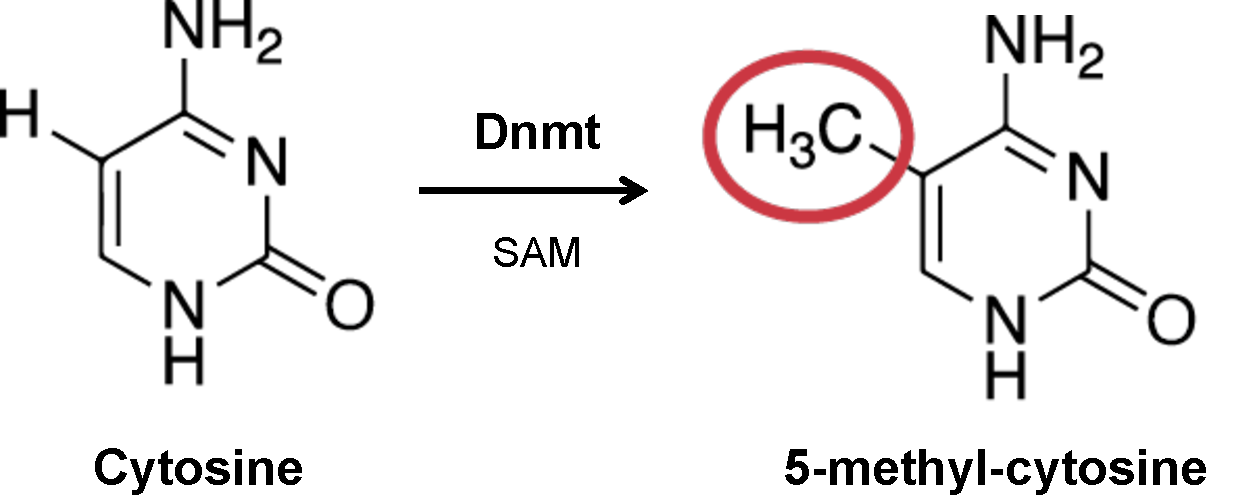
\includegraphics[width=0.7\textwidth]{cpg}
\caption[Chemical reaction of cytosine to 5-methylcytosine.]{Chemical reaction of cytosine to 5-methylcytosine. Cytosine is converted to 5-methylcytosine (5mC) by the transfer of a methyl group from S-adenosyl-L-methionine (SAM) to the fifth carbon atom of the cytosine pyrimidine ring, catalyzed by enzymes of the DNA methyltransferase (Dnmt) family.}
\label{fig:intro_cpg}
\end{figure}

DNA methylation can also occur at non-CpG sites, including CHG and CHH sites, where H can be any nucleotide except for G. Non-CpG methylation has been reported in plants, fungi, and embryonic stem cells (ESCs), but the functional relevance of non-CpG methylation is still unclear~\citep{jones_functions_2012,ziller_genomic_2011,ramsahoye_non-cpg_2000,shirane_mouse_2013}.

DNA methylation is established during embryonic development by a series of de novo methylation and demethylation events. Enzymes of the DNA methyltransferase (Dnmt) family catalyse DNA methylation by transferring the methyl-group of S-adenosyl-L-methionine (SAM) to cytosine (\Cref{fig:intro_cpg}). Three active Dnmt enzymes have been identified in mammals: Dnmt1, Dnmt3a, and Dnmt3b. Although these enzymes are structurally similar, they serve different functions and are expressed at different time points during embryonic development~\citep{moore_dna_2013,jones_rethinking_2009,bestor_notes_2015}. Dnmt3a and Dnmt3b are also known as `de novo Dnmt', since they establish new tissue-specific methylation patterns during embryogenesis (\Cref{fig:intro_dnmt}~(a)). Whereas Dnmt3a is ubiquitously expressed in all cell types, Dnmt3b is only expressed in differentiating cells. Dnmt1 is also known as `maintenance Dnmt', since it maintains DNA methylation during cell division and cell differentiation. Dnmt1 preferentially binds to hemi-methylated DNA during DNA replication, and methylates cytosine residues on the newly synthesized DNA strand (\Cref{fig:intro_dnmt}~(b)). Dnmt1 regulates genomic imprinting by repressing either the maternal or paternal copy of genes, and is involved in DNA repair.
\begin{figure}[htbp!]
\centering
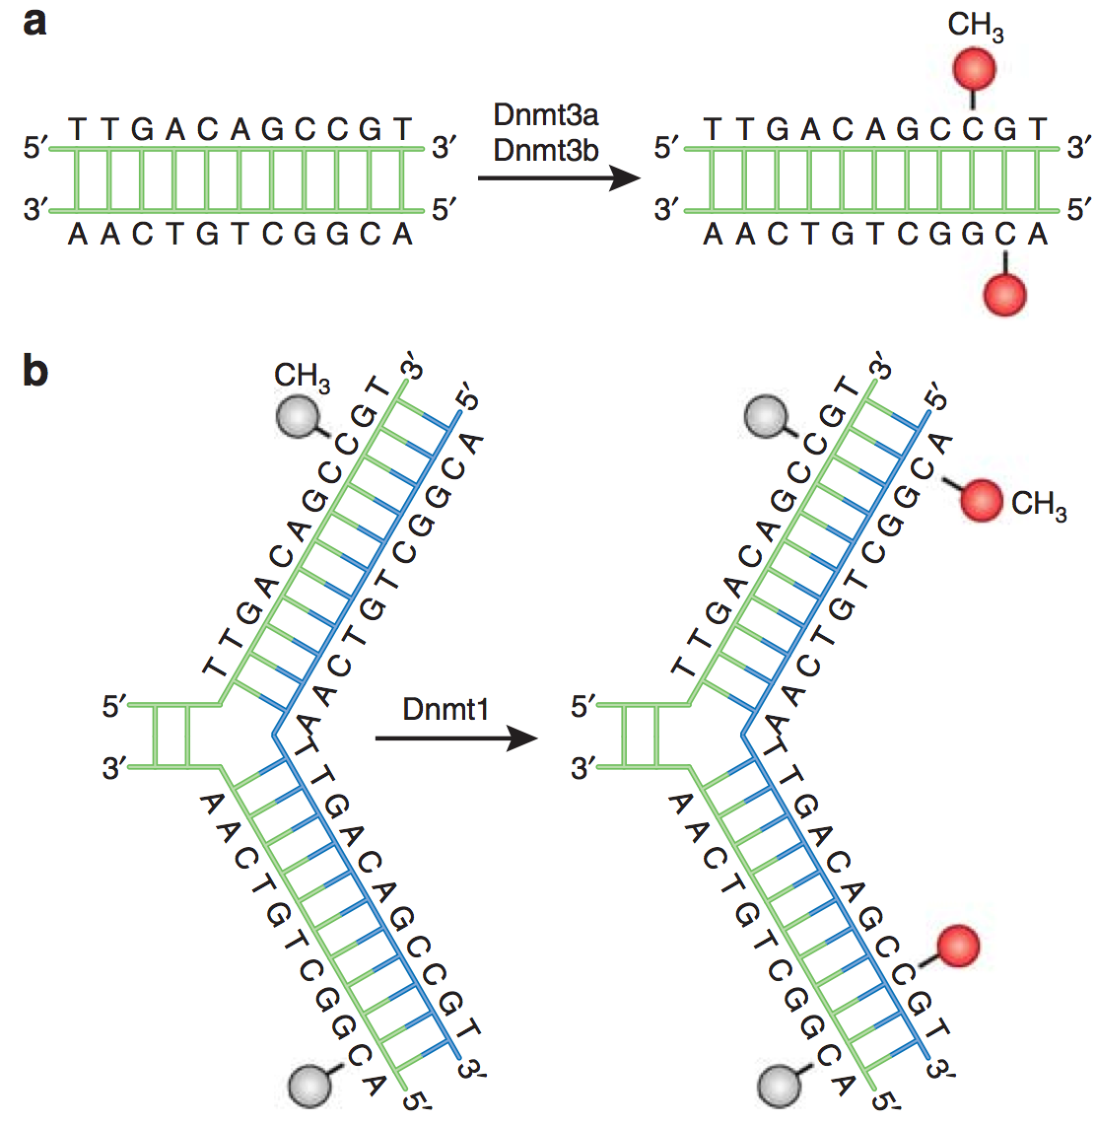
\includegraphics[width=0.6\textwidth]{dnmt}
\caption[DNA methyltransferase enzymes.]{DNA methyltransferase enzymes. DNA methyltransferase (Dnmt) is a family of enzymes that catalyzes the conversion from cytosine to 5-methylcytosine. (a) Dnmt3a and Dnmt3b can establish new methylation patterns by methylating DNA de novo. (b) Dnmt1 maintains existing methylation patterns during cell replication by methylating hemi-methylated DNA. It binds close to the replication fork and methylates CpG sites on the newly synthesized daughter strand at CpG sites that are methylated on the parent strand. Source: \citet{moore_dna_2013}.}
\label{fig:intro_dnmt}
\end{figure}

Although DNA methylation is primarily established during embryonic development and maintained in replicating cells, methylation patterns can be changed by environmental factors and stochastic fluctuations. DNA methylation can be erased passively by the inhibition of Dnmt1, resulting in gradually decreasing methylation levels in differentiating cells. Active demethylation can occur in both differentiating and non-differentiating cells, and involves the removal of the methyl group from 5mC through are series of chemical reactions~\citep{mayer_embryogenesis:_2000,zhang_active_2007}.

\section{Functions of DNA methylation} \label{sec:intro_fun}

The function of DNA methylation varies between genomic contexts~\citep{bestor_notes_2015,moore_dna_2013,jones_functions_2012,bird_dna_2002}. Promoter methylation has been associated with regulatory effects on gene expression~\citep{moore_dna_2013,jones_functions_2012,bird_dna_2002}. About 70\% of all promoters in the human genome are CGI promoters, i.e. promoters that are overlapped by at least own CGI. Promoter CGIs are evolutionary conserved, which indicates their functional importance. Most promoter CGIs are unmethylated and nucleosome depleted, which has been associated with increased DNA accessibility and gene expression levels~\citep{moore_dna_2013}. The high GC density in CGI promoters has further been associated with an increased binding of transcription factors that regulate gene expression~\citep{moore_dna_2013}. The methylation of promoter CGIs blocks RNA polymerases and thus inhibits gene expression. This is important to variably activate and deactivate genes during cell differentiation and to establish tissue-specific expression patterns synchronized with other epigenetic factors. CGI promoter methylation further regulates imprinting by inhibiting the expression of either the maternal or paternal allele of genes. Another import role of CGI promoter methylation is X chromosome inactivation—the deactivation of one copy of the X chromosome in female mammalian cells by bulk methylation of all gene promoters~\citep{bestor_notes_2015}.

Unlike CGI promoters, which are predominantly unmethylated, non-CGI promoters are more heterogeneous. Although evidence exists that non-CGI promoter methylation may be involved in tissue-specific gene regulation~\citep{moore_dna_2013,jones_functions_2012}, the exact regulatory mechanisms are still unknown.

Intergenic regions are CpG poor and tend to be methylated. Methylation in intergenic regions is important for repressing transposable and viral elements~\citep{moore_dna_2013,jones_functions_2012,robertson_dna_2005}, which account for about 45\% of the genomic DNA in mammalian cells. These elements are either repressed by CpG methylation or inactive due to C$\rightarrow$T mutations acquired by the spontaneous deamination of 5mC. For example, the intracisternal A-particle (IAP) is a detrimental retrovirus that resides in the mouse genome~\citep{walsh_cytosine_1999}. IAPs are highly methylated by Dnmt1 and thereby repressed. Knockout of Dnmt1 induces demethylation and hence the expression and IAPs and cell death~\citep{walsh_cytosine_1999,hutnick_repression_2010}.

Gene bodies are CpG poor and mostly methylated similar to intergenetic regions. Gene body methylation likewise serves as a mechanism to repress transposable and viral elements~\citep{moore_dna_2013,jones_functions_2012,robertson_dna_2005}. Although gene bodies are generally CpG poor, they can contain CGIs. However, the methylation of gene body CGIs does not block transcription, unlike promoter CGIs, and the implications of gene body methylation in gene regulation is still unclear: Whereas some studies found positive associations between gene body methylation and gene expression, others have reported negative associations in slowly dividing and non-dividing cells.

Gene enhancers are relatively short (50-1500~bp) genetic elements that promote gene expression~\citep{blackwood_going_1998,pennacchio_enhancers:_2013}. They tend to be GC poor and to have heterogeneous methylation levels. For example, low methylated regions (LMRs~\citep{stadler_dna-binding_2011}) are indicative of distal enhancer elements. They are characterized by an average methylation rate of 30\%, which can fluctuate considerably during cell differentiation. Although some studies found negative associations between enhancer methylation and gene expression, further studies are needed to explore the regulatory function of these associations.

Insulators are genetic elements that block promoter-enhancer interactions~\citep{burgess-beusse_insulation_2002}. Insulators are bound by the CTCF zinc finger protein and transported close to gene promoters by looping of the DNA strand. Insulator methylation can block CTCF binding, and thereby support promoter-enhancer interactions. However, the roles of insulator methylation are still unclear~\citep{moore_dna_2013,jones_functions_2012}.

\section{Protocols for methylation profiling} \label{sec:intro_proto}

Several methods have been developed for profiling DNA methylation, which can be broadly grouped into protocols based on enzymatic digestion, affinity enrichment, and bisulfite conversion~\citep{yong_profiling_2016,schwartzman_single-cell_2015,plongthongkum_advances_2014,huang_profiling_2010,laird_principles_2010-1}.

Protocols based on enzymatic digestion leverage methylation-sensitive restriction enzymes (MREs), which have differential digestion properties for methylated and unmethylated CpG sites. The two most common MREs are HpaII, which cleaves unmethylated CpG sites, and Msp1, which cleaves methylated CpG sites. Protocols proceed by enzymatically digesting DNA using a specific MRE, followed by DNA methylation quantification using either array hybridization (MRE-chip~\citep{chittur_help_2010}) or sequencing (MRE-seq~\citep{maunakea_conserved_2010}). Enzymatic digestion-based approaches are cost-effective and enable genome-wide methylation profiling. However, their resolution is limited to regions adjacent to MRE recognition sites, and they cannot quantify the methylation level of single CpG sites.

Affinity enrichment-based protocols enrich for methylated DNA fragments by either methyl-binding domain (MBD) proteins or antibodies that target 5mC. Methylated DNA immunoprecipitation (MeDIP) uses anti-methylcytosine antibodies to bind and quantify 5mC. The protocol consists of DNA fragmentation by sonication, enrichment of methylated fragments by immunoprecipitation, and methylation quantification by either array hybridization (MeDIP-chip~\citep{park-sarge_methylated_2009}) or sequencing (MeDIP-seq~\citep{brinkman_whole-genome_2010}). MeDIP is cost effective and can differentiate between CpG, CHG, and CHH methylation contexts. Since MeDIP only requires small amounts of DNA starting material, it is further applicable to small cell populations. On the downside, the resolution of MeDIP is limited to 100-300~bp long fragments and the method is biased towards hypermethylated regions.

Protocols based on bisulfite conversion enable quantifying the methylation levels of single CpG sites. Protocols involve the fragmentation of DNA using sonication or enzymatic digestion and the treatment of DNA fragments with sodium bisulfite. Sodium bisulfite converts unmethylated cytosine to uracil, which eventually turns into thymine by PCR amplification. The resulting C$\rightarrow$T conversions are detected either using array hybridization or next generation sequencing and thereby CpG sites classified as methylated or unmethylated.

\begin{figure}[htbp!]
\centering
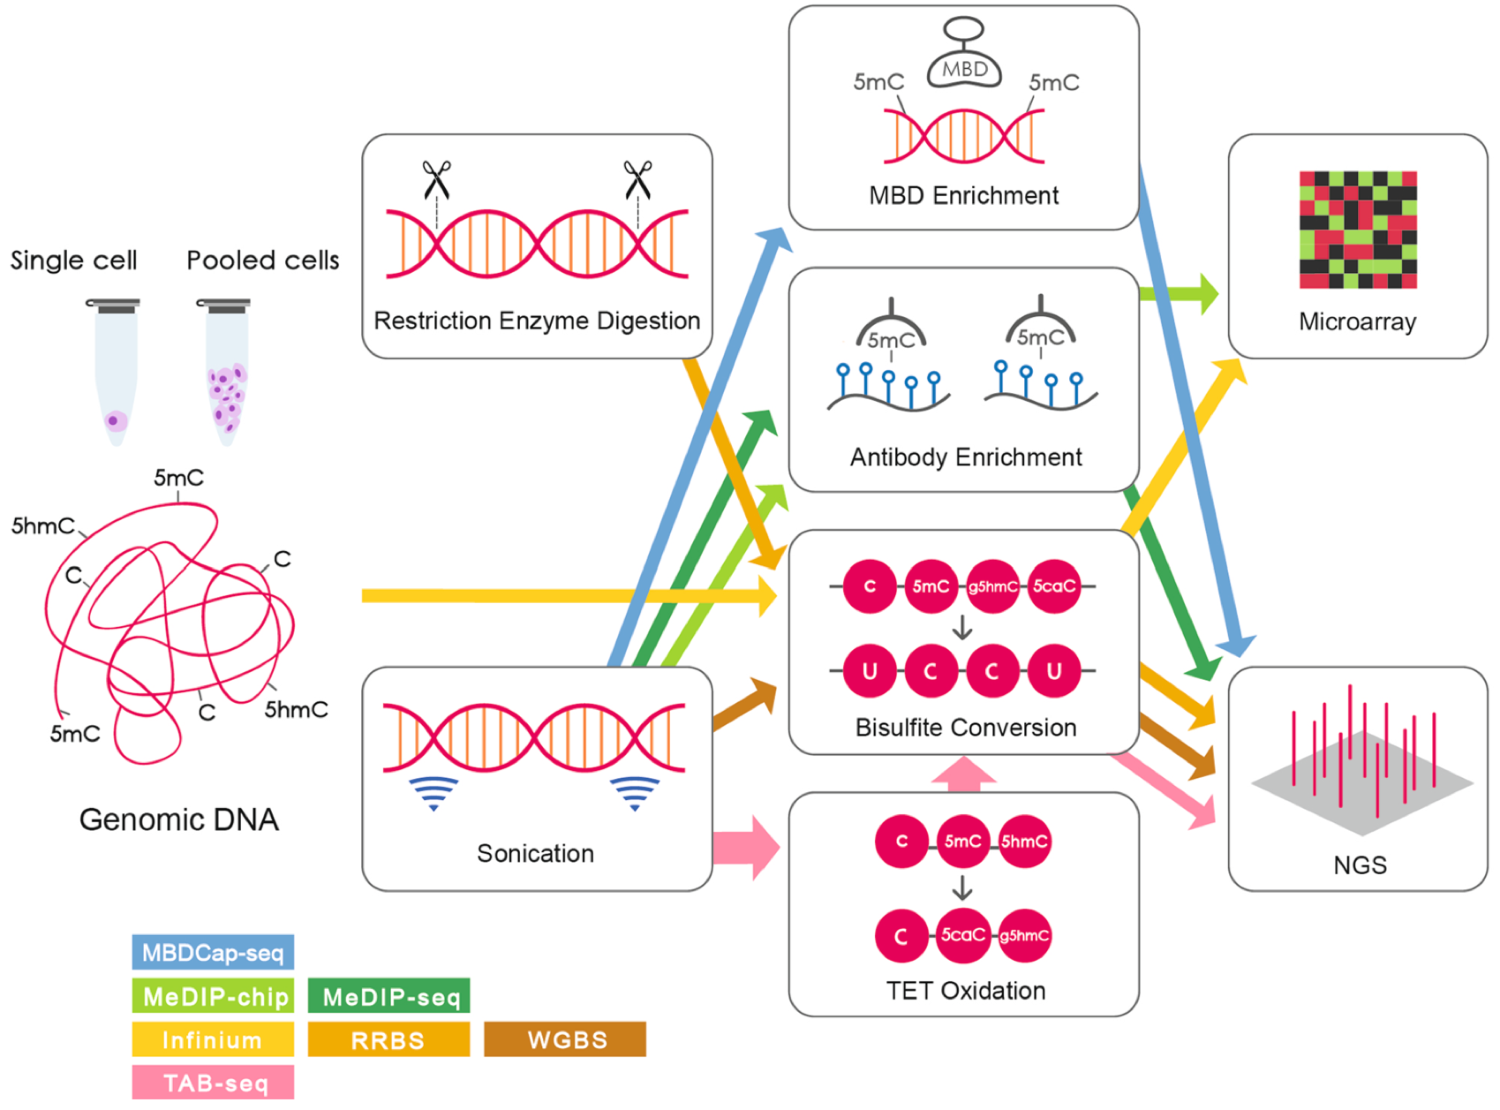
\includegraphics[width=0.8\textwidth]{seq}
\caption[Workflow of DNA methylation profiling protocols.]{Workflow of DNA methylation profiling protocols. DNA starting material is extracted from either a bulk population of cells or a single cell and fragmented by enzymatic digestion or sonication. Enrichment based profiling protocols enrich for methylated DNA fragments by either methyl-binding domain (MBD) proteins or antibodies. Bisulfite conversion-based protocols treat DNA fragments by bisulfite to convert unmethylated cytosine to thymine. DNA methylation levels are quantified by microarray hybridization of next generation sequencing (NGS). Source: \citet{yong_profiling_2016}.}
\label{fig:intro_seq}
\end{figure}

Illumina's 450K bead-chip is the most widely used bisulfite microarray for profiling DNA methylation in human, which integrates bisulfite treatment, PCR amplification, and hybridization~\citep{bibikova_high_2011-1}. Two distinct primers are used to distinguish between methylated and unmethylated fragments, which are labelled by different fluorescence dyes and hybridized to bead arrays.  The chip probes about 450K CpG sites in the human genome, which cover most CGIs. It is cost-effective but biased towards CpG dense contexts.

Whole genome bisulfite sequencing (BS-seq~\citep{urich_methylc-seq_2015}) detects C$\rightarrow$T conversions by sequencing bisulfite treated fragments, and aligning the sequenced fragments back to a reference genome. BS-seq is considered as the gold standard protocol since it can profile DNA methylation at single cytosine resolution genome-wide, and can differentiate between CpG, CHG, and CHH contexts. However, BS-seq is more expensive since it requires genome-wide deep sequencing of bisulfite-treated fragments.

Reduces representation bisulfite sequencing (RRBS-seq~\citep{meissner_genome-scale_2008-1,smith_high-throughput_2009}) is a cost-effective alternative to BS-seq, which quantifies DNA methylation only for a subset of genomic fragments. The method is based on the observation that Msp1-digested DNA fragments of size 20-200~bp cover about 85\% of all CpG sites, including most CGIs. By sequencing only bisulfite treated fragments of size 20-200~bp, RRBS-seq is more cost effective than BS-seq, however, biased towards CpG dense regions.

As a consequence of DNA degradation by multiple purification steps and bisulfite treatment, conventional bisulfite protocols require relative large amounts of DNA starting material, which is usually obtained from a bulk population of thousands or millions of cells. Hence, bulk protocols quantify average methylation levels and cannot assess methylation heterogeneity between cells.

Recent technological advances enabled to reduced DNA degradation and thereby to profile DNA methylation in single cells. \citet{guo_profiling_2015} adapted the RRBS protocol by integrating all experimental steps before PCR amplification into a single tube. Their reduced representation protocol (scRRBS-seq) probes about 1-10\% of all CpG sites, is cost-effective but limited to CpG dense regions similar to RRBS-seq. We and colleagues proposed scBS-seq~\citep{smallwood_single-cell_2014}, the first protocol to profile DNA methylation in single cells genome-wide. scBS-seq reduces DNA degradation by a modification of the post bisulfite adaptor tagging (PBAT~\citep{miura_amplification-free_2012-1}) protocol. Here, the DNA is treated with bisulfite prior to adapter ligation instead of afterwards, which simultaneously fragments the DNA and converts unmethylated cytosine to thymine. The protocol covers about 10-30\% of all CpG sites per cell and will be described in more detail in \cref{sec:bs}.

Single-cell protocols have multiple advantages over bulk protocols~\citep{schwartzman_single-cell_2015}. First, they enable the study of DNA methylation variability and differences between individual cells, such as ESCs and cancer cells. Second, single-cell protocols for parallel profiling of multiple data modalities, e.g. DNA methylation and gene expression, provide the potential to analyse the regulatory relationship between these data modalities. Third, single-cell protocols are applicable to small cell populations that cannot be profiled by bulk protocols due to insufficient DNA starting material. On the downside, single-cell protocols are limited by incomplete CpG coverage and high levels of technical noise, which render downstream analyses challenging. We therefore developed computational methods for the genome-wide analysis of single-cell DNA methylation profiling data, which will be described in the subsequent chapters.

\section{Contributions} \label{sec:intro_contrib}

In this chapter, we have introduced DNA methylation, its roles in biology, and protocols for profiling DNA methylation in bulk populations of cells and single cells. Data from single-cell profiling protocols offer great potential for studying intercellular differences but difficult to analyse due to high levels of technical noise and incomplete CpG coverage. This thesis contributes deep neural networks and statistical methods for the analysis of single-cell DNA methylation data, which are applicable genome-wide, account for incomplete CpG coverage, and provide mechanistic insights.

In \cref{sec:dl}, we will introduce deep neural networks for computational biology. We will contrast deep neural networks with conventional machine learning models, present different network architectures, and review applications in computational biology. Chapter two forms the foundation of chapter four and five on deep neural networks for predicting and analysing DNA methylation. The work presented in this chapter is based on \citet{angermueller_deep_2016}.

In \cref{sec:pro}, we will present protocols and computational methods for the genome-wide analysis of single-cell DNA methylation. We will first describe scBS-seq, a protocol that enables profiling DNA methylation in single cells genome-wide, as well as a statistical model for assessing DNA methylation heterogeneity between cells. We will subsequently describe scM\&T-seq, an extension of scBS-seq that enables parallel profiling of DNA methylation and gene expression in single cells, as well as methods for quantifying associations between DNA methylation and gene expression. The work presented in this chapter is based on \citet{smallwood_single-cell_2014} and \citet{angermueller_parallel_2016}.

In \cref{sec:dcpg}, we will present DeepCpG, a deep neural network model for predicting DNA methylation in single cells. We will discuss the limitations of existing methods, describe the DeepCpG model architecture, and show that DeepCpG yields considerably more accurate predictions than existing methods. The work presented in this chapter is based on \citet{angermueller_accurate_2017}.

In \cref{sec:dcpg_ana}, we will describe approaches for analysing DNA methylation using DeepCpG. We will show that DeepCpG can be applied to discover DNA sequence motifs that are associated with methylation states, to identify variance-associated motifs, and to estimate the effect of single nucleotide mutations on DNA methylation. The work presented in this chapter is based on \citet{angermueller_accurate_2017}.

In \cref{sec:sum}, we will summarize this thesis and provide an outlook on future research.

%!TEX root = ../thesis.tex
%*******************************************************************************
%****************************** Second Chapter *********************************
%*******************************************************************************


\chapter{Deep learning for computational biology} \label{sec:dl}

\ifpdf
    \graphicspath{{Chapter2/Figs/Raster/}{Chapter2/Figs/PDF/}{Chapter2/Figs/}}
\else
    \graphicspath{{Chapter2/Figs/Vector/}{Chapter2/Figs/}}
\fi

Machine learning is a pillar of modern computational biology. The latest machine learning methods garnering significant attention are deep neural networks, which have led to breakthroughs in various fields~\citep{lecun_deep_2015,schmidhuber_deep_2015,bengio_representation_2013}, including computational biology~\citep{alipanahi_predicting_2015,dahl_multi-task_2014,eickholt_dndisorder:_2013,kelley_basset:_2016,leung_deep_2014,sonderby_protein_2014,wang_chromatin_2015,zhou_predicting_2015}. In the following, we will introduce deep neural networks and review applications in regulatory genomics and biological image analysis. This chapter forms the foundation of \cref{sec:dcpg} and \cref{sec:dcpg_ana}, which will describe methods based on deep neural networks for predicting and analysing DNA methylation. The presented work is based on \citet{angermueller_deep_2016}, which was joint work of Christof Angermueller, Tanel P\"arnamaa, Leopold Parts, and Oliver Stegle.

\begin{center}
\begin{minipage}{.9\linewidth}
\underline{Individual contributions}: Christof Angermueller and Oliver Stegle reviewed applications of deep neural networks in regulatory genomics and summarized off-the-shelf tools and practical considerations. Tanel P\"arnamaa and Leopold Parts reviewed applications of deep neural network in biological image analysis. All authors wrote the manuscript.
\end{minipage}
\end{center}

\section{Machine learning}

Machine learning methods are general-purpose approaches to learn functional relationships from data without the need to define them a priori~\citep{hastie_elements_2005,michalski_machine_2013,murphy_machine_2012}. In computational biology, their appeal is the ability to derive predictive models without a need for strong assumptions about underlying mechanisms, which are frequently unknown or insufficiently defined. As a case in point, the most accurate prediction of gene expression levels is currently made from a broad set of epigenetic features using sparse linear models~\citep{cheng_statistical_2011,karlic_histone_2010} or random forests~\citep{li_using_2015}; how the selected features determine the transcript levels remains an active research topic. Predictions in genomics~\citep{libbrecht_machine_2015,martens_predicting_2016}, proteomics~\citep{swan_application_2013}, metabolomics~\citep{kell_metabolomics_2005}, or sensitivity to compounds~\citep{eduati_prediction_2015} all rely on machine learning approaches as a key ingredient.

Most of these applications can be described within the canonical machine learning workflow, which involves four steps: data cleaning and pre-processing, feature extraction, model fitting, and evaluation (\Cref{fig:dl_ml}~(a)). It is customary to denote one data sample, including all covariates and features as input $x$ (usually a vector of numbers), and label it with its response variable or output value $y$ (usually a single number) when available.

A supervised machine learning model aims to learn a function $y=f(x)$ from a list of training pairs $(x_1,y_1), (x_2,y_2),\ldots$ for which data are recorded (\Cref{fig:dl_ml}~(b)). One typical application in biology is to predict the viability of a cancer cell line when exposed to a chosen drug~\citep{eduati_prediction_2015,menden_machine_2013}. The input features $x$ would capture somatic sequence variants of the cell line, chemical makeup of the drug, and its concentration, which together with the measured viability (output label $y$) can be used to train a support vector machine, a random forest classifier or a related method (functional relationship $f$). Given a new cell line (unlabelled data sample $x^*$) in the future, the learned function predicts its survival $y^*=f(x^*)$, even if $f$ resembles more of a black box, and its inner workings of why particular mutation combinations influence cell growth are not easily interpreted. Both regression (where $y$ is a real number), and classification (where $y$ is a categorical class label) can be viewed in this way. As a counterpart, unsupervised machine learning approaches aim to discover patterns from the data samples $x$ itself, without the need for output labels $y$. Methods such as clustering, principal components analysis, and outlier detection are typical examples of unsupervised models applied to biological data.

\begin{figure}[htbp!]
\centering
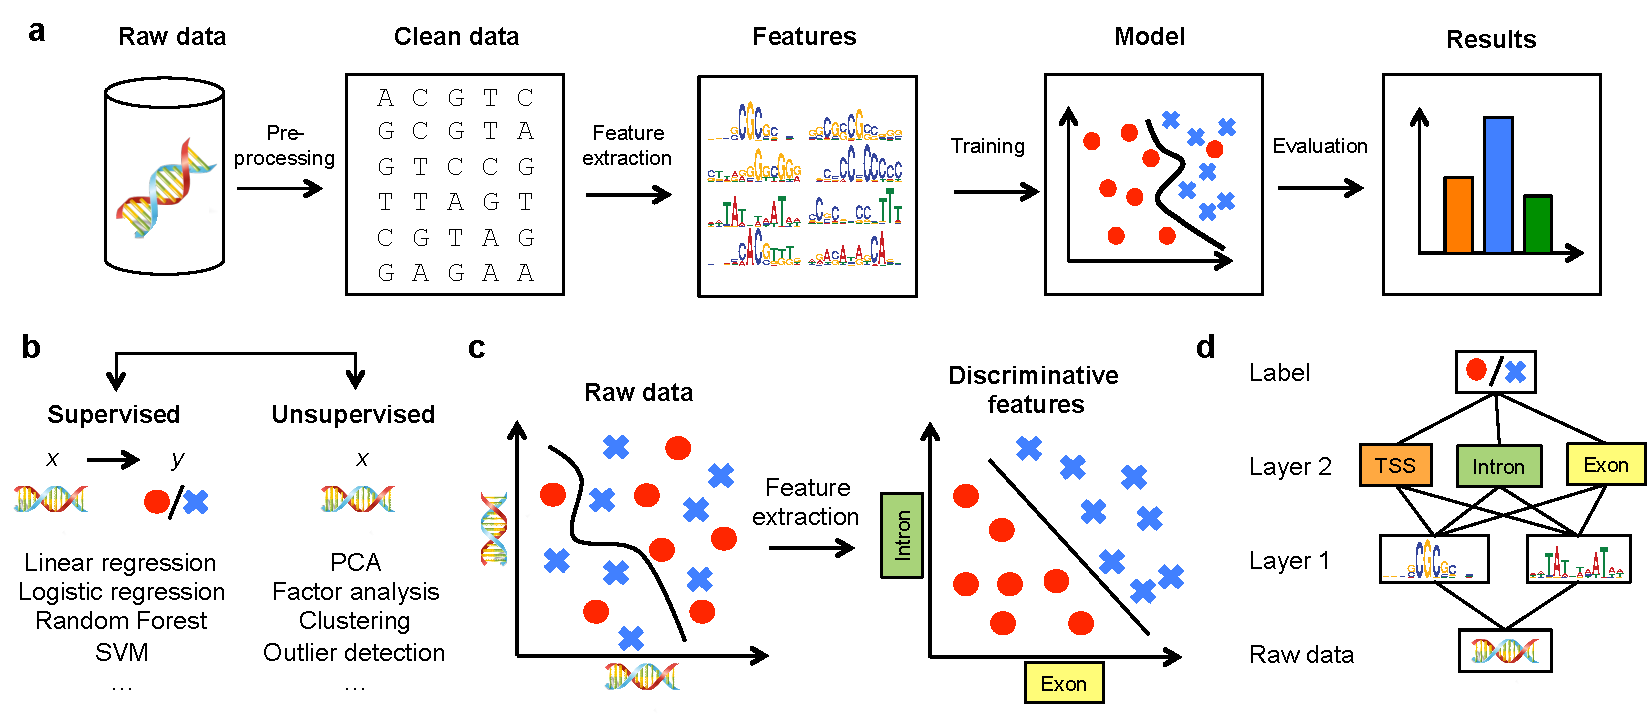
\includegraphics[width=1.0\textwidth]{ml}
\caption[Machine learning and representation learning.]{Machine learning and representation learning. (a) The classical machine learning workflow can be broken down into four steps: data pre-processing, feature extraction, model learning, and model evaluation. (b) Supervised machine learning methods relate input features $x$ to an output label $y$, whereas unsupervised method learn factors about $x$ without observed labels. (c) Raw input data are often high dimensional and related to the corresponding label in a complicated way, which is challenging for many classical machine learning algorithms (left plot). Alternatively, higher-level features extracted using a deep model may be able to better discriminate between classes (right plot). (d) Deep networks use a hierarchical structure to learn increasingly abstract feature representations from the raw data.}
\label{fig:dl_ml}
\end{figure}

The inputs $x$, calculated from the raw data, represent what the model `sees about the world', and their choice is highly problem specific (\Cref{fig:dl_ml}~(c)). Deriving most informative features is essential for performance, but the process can be labour-intensive and requires domain knowledge. This bottleneck is especially limiting for high dimensional data; even computational feature selection methods do not scale to assess the utility of vast number of possible input combinations. A major recent advance in machine learning is automating this critical step by learning a suitable representation of the data with deep artificial neural networks~\citep{bengio_representation_2013,lecun_deep_2015,schmidhuber_deep_2015} (\Cref{fig:dl_ml}~(d)). Briefly, a deep neural network takes the raw data at the lowest (input) layer, and transforms them into increasingly abstract feature representations by successively combining outputs from the preceding layer in a data-driven manner, encapsulating highly complicated functions in the process (\Cref{fig:dl_ann}). Deep learning is now one of the most active fields in machine learning and has been shown to improve performance in image- and speech recognition~\citep{deng_deep_2015,graves_generating_2013,hinton_deep_2012,krizhevsky_imagenet_2012,zeiler_visualizing_2014-1}, natural language understanding~\citep{bahdanau_neural_2014,lipton_critical_2015,sutskever_sequence_2014,xiong_dynamic_2016}, and most recently, in computational biology~\citep{alipanahi_predicting_2015,dahl_multi-task_2014,eickholt_dndisorder:_2013,kelley_basset:_2016,leung_deep_2014,sonderby_protein_2014,wang_chromatin_2015,zhou_predicting_2015}.

The potential of deep learning in high throughput biology is clear: in principle, it allows to better exploit the availability of increasingly large and high-dimensional datasets (e.g. from DNA sequencing, RNA measurements, flow cytometry, or automated microscopy) by training complex networks with multiple layers that capture their internal structure (\Cref{fig:dl_ml}~(c)). The learned networks discover high-level features, improve performance over traditional models, increase interpretability and provide additional understanding about the structure of the biological data.

In the following, we will describe prominent deep neural network architectures and review applications in regulatory genomics and biological image analysis. We will further provide practical pointers, summarise current software solutions, and give recommendations for applying them to data. Finally, we will discuss both the potential and possible pitfalls of deep learning and contrast deep learning with traditional machine learning and statistical analysis.


\section{Artificial neural networks}

An artificial neural network, initially inspired by neural networks in the brain~\citep{farley_simulation_1954,mcculloch_logical_1943,rosenblatt_perceptron:_1958} consists of layers of interconnected compute units (neurons). In the canonical configuration, the network receives data in an input layer, which are then transformed in a nonlinear way through multiple hidden layers, before final outputs are computed in the output layer (\Cref{fig:dl_ann}~(a)). Neurons in a hidden or output layer are connected to all neurons in the previous layer. Each neuron computes a weighted sum of its inputs, and applies a nonlinear activation function to calculate its output (\Cref{fig:dl_ann}~(b)). The most popular activation function is the Rectified linear unit (ReLU; \Cref{fig:dl_ann}~(b)), since it allows faster learning compared to alternatives (e.g. sigmoid or tanh unit)~\citep{glorot_deep_2011}. The depth of a neural network corresponds to the number of hidden layers, and the width to the maximum number of neurons in one of its layers. As it became possible to train networks with larger numbers of hidden layers, artificial neural networks were rebranded to `deep networks'.

\begin{figure}[htbp!]
\centering
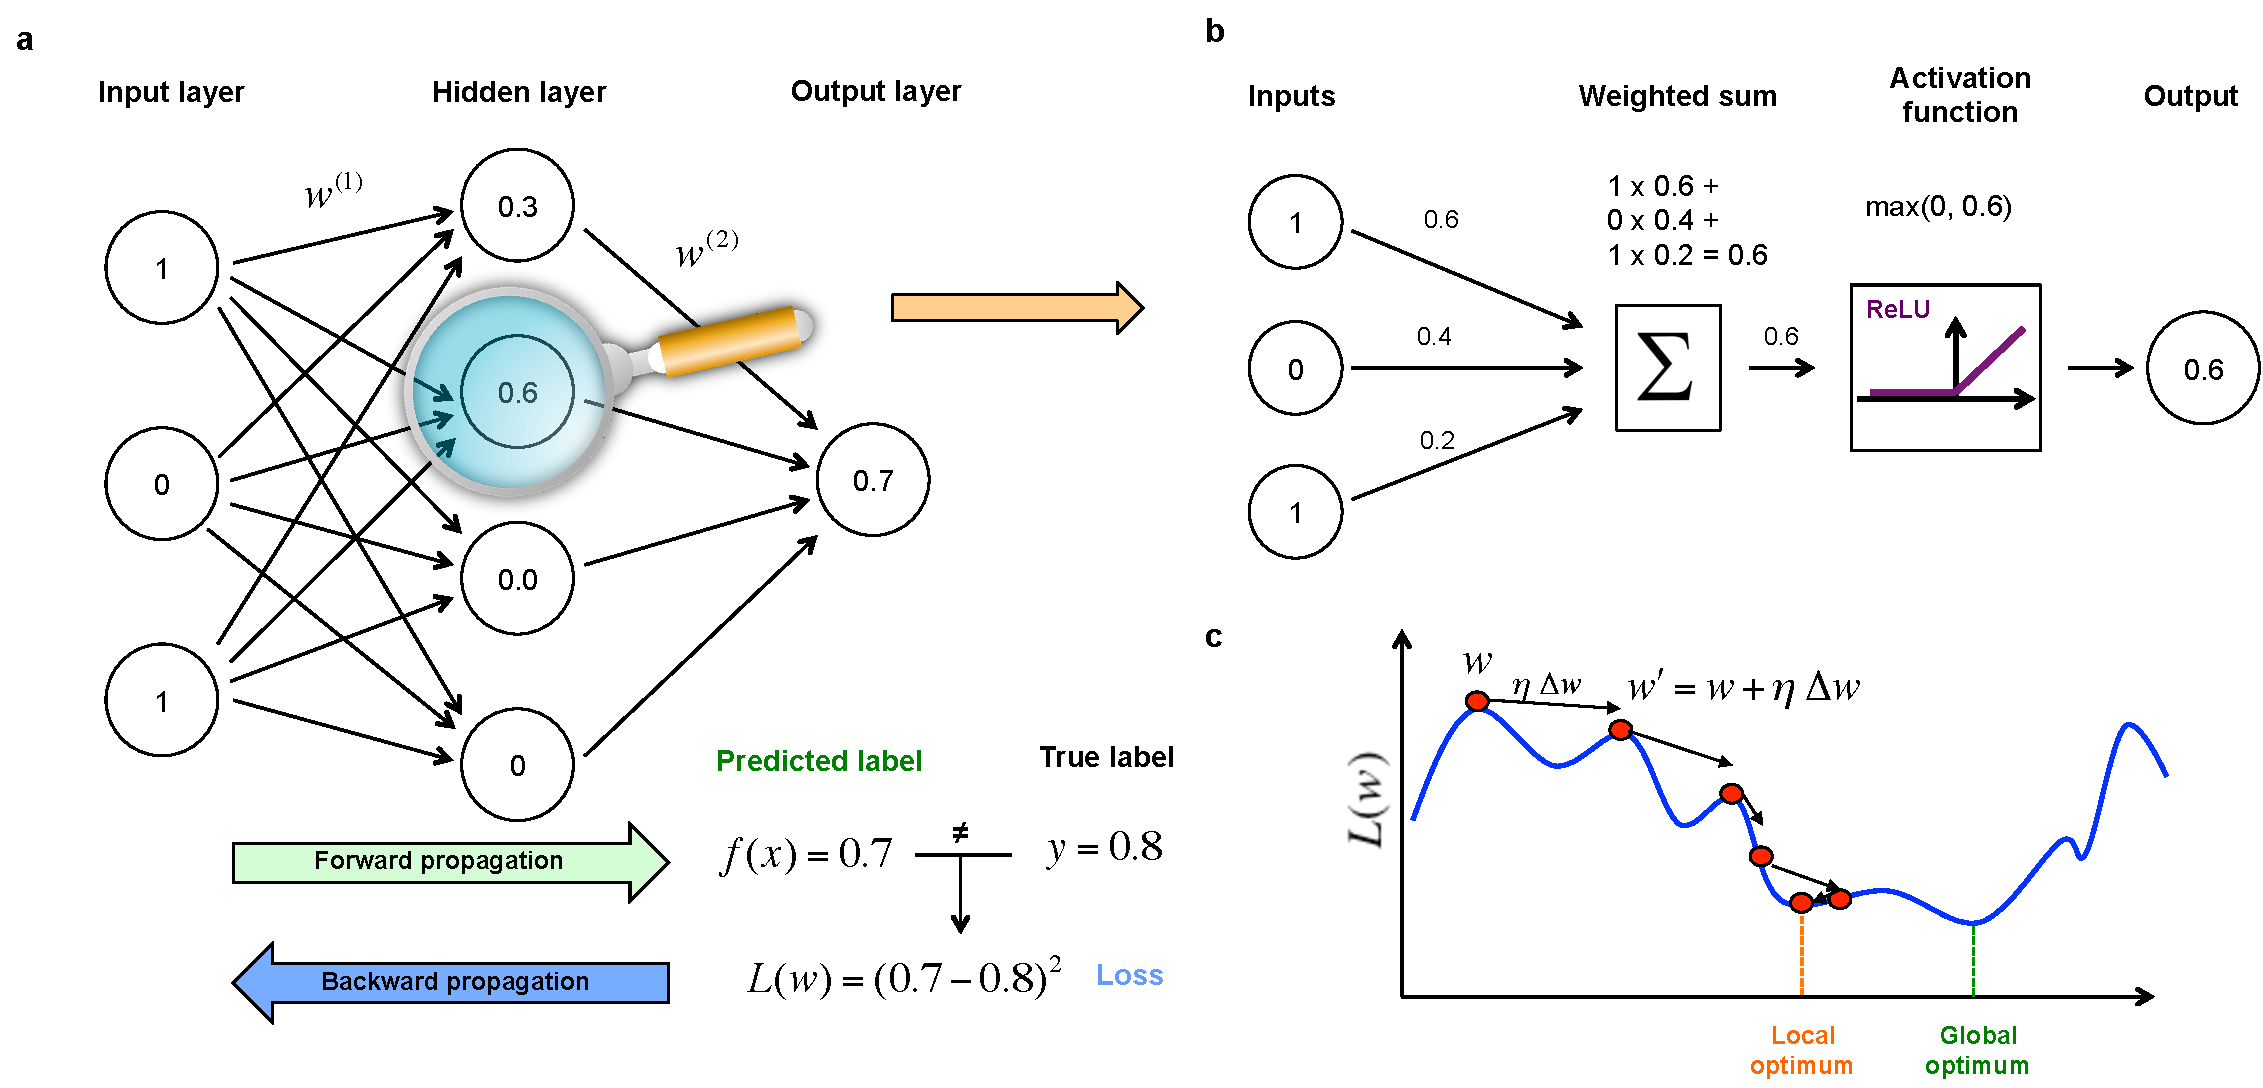
\includegraphics[width=1.0\textwidth]{ann}
\caption[Building blocks and learning principles of a neural network.]{Building blocks and learning principles of a neural network. (a) Fully connected feedforward neural network with one input layer, hidden layer, and output layer.  Each layer $i$ consists of neurons which are connected to all neurons in the previous layer with weights $w(i)$. Given input $x$, neuron activations are calculated and forward propagated to the output layer to obtain a prediction $f(x)$. (b) Zoom-in view into one neuron, which computes the weighted sum of its inputs and applies a rectification function that thresholds negative signals to $0$, and passes through positive signal. (c) Gradient-based optimization of the loss function $L(w)$. In each step, the current weight vector (red dot) is moved along the direction of steepest descent $\Delta w$ (direction arrow) by learning rate $\eta$ (length of vector). Decaying the learning rate over time allows to explore different domains of the loss function by jumping over valleys at the beginning of the training (left side), and fine-tune parameters with smaller learning rates in later stages of the model training.}
\label{fig:dl_ann}
\end{figure}

The weights between neurons are free parameters that capture the model's representation of the data, and are learned from input/output samples. Learning minimizes a loss function that measures the fit of the model output to the true label of a sample (\Cref{fig:dl_ann}~(a), bottom). This minimization is challenging, since the loss function is high dimensional and non-convex, similar to a landscape with many hills and valleys (\Cref{fig:dl_ann}~(c)). It took several decades before the backward propagation algorithm was first applied to compute a loss function gradient via chain rule for derivatives~\citep{rumelhart_learning_1988}, ultimately enabling efficient training of neural networks using stochastic gradient descent. During learning, the predicted label is compared with the true label to compute a loss for the current set of model weights. The loss is then backward propagated through the network to compute the gradients of the loss function and update (\Cref{fig:dl_ann}~(a)). While learning in deep neural networks remains an active area of research, existing software packages (\Cref{tab:dl_tools}) can already be applied without knowledge of the mathematical details involved.

Several architectures have been developed for specific applications, which differ in the way neurons are arranged. These include the convolutional neural network for images, the recurrent neural network for sequential data~\citep{lipton_critical_2015,sutskever_training_2013}, or the restricted Boltzmann machine~\citep{hinton_practical_2012,salakhutdinov_efficient_2010} and autoencoder~\citep{alain_regularized_2012,hinton_reducing_2006,kingma_auto-encoding_2013} for unsupervised learning. The multilayer perceptron, convolutional neural network, and recurrent neural network are most widely used in biology, and will be outlined in the following.


\subsection{Multilayer perceptron}

The multilayer perceptron (MLP)~\citep{rosenblatt_perceptron:_1958} is the most basic artificial neural network, which consists of a sequence of fully-connected layers. Specifically, all neurons in a layer are connected to all neurons in the previous layer (\Cref{fig:dl_ann}~(a)). However, no connections exits between neurons within the same layer, as opposed to the recurrent neural network (\Cref{sec:dl_rnn}). A MLP with many layers and neurons can be very powerful, but is limited by a high number of parameters, which scales quadratically with the number of neurons per layer. Specialized architectures have been developed to reduce the number of parameters and avoid overfitting, which include the convolutional neural network.


\subsection{Convolutional neural network} \label{sec:dl_cnn}

Convolutional neural networks (CNNs) were originally inspired by cognitive neuroscience and Hubel and Wiesel's seminal work on the cat's visual cortex, which was found to have simple neurons that respond to small motifs in the visual field, and complex neurons that respond to larger ones~\citep{hubel_shape_1963,hubel_period_1970}.

CNNs are designed to model input data in the form of multi-dimensional arrays, such as two-dimensional images with three colour channels~\citep{he_deep_2015,jarrett_what_2009,krizhevsky_imagenet_2012,lecun_backpropagation_1989,szegedy_rethinking_2015,zeiler_visualizing_2014-1}, or one-dimensional genomic sequences with one channel per nucleotide~\citep{alipanahi_predicting_2015,angermueller_accurate_2017,kelley_basset:_2016,zhou_predicting_2015}. The high dimensionality of these data (up to millions of pixels for high-resolution images) render training a fully connected neural network challenging, as the number of parameters of such a model would typically exceed the number of training data to fit them. To circumvent this, CNNs make additional assumptions on the structure of the network, thereby reducing the effective number of parameters to learn.

\begin{figure}[htbp!]
\centering
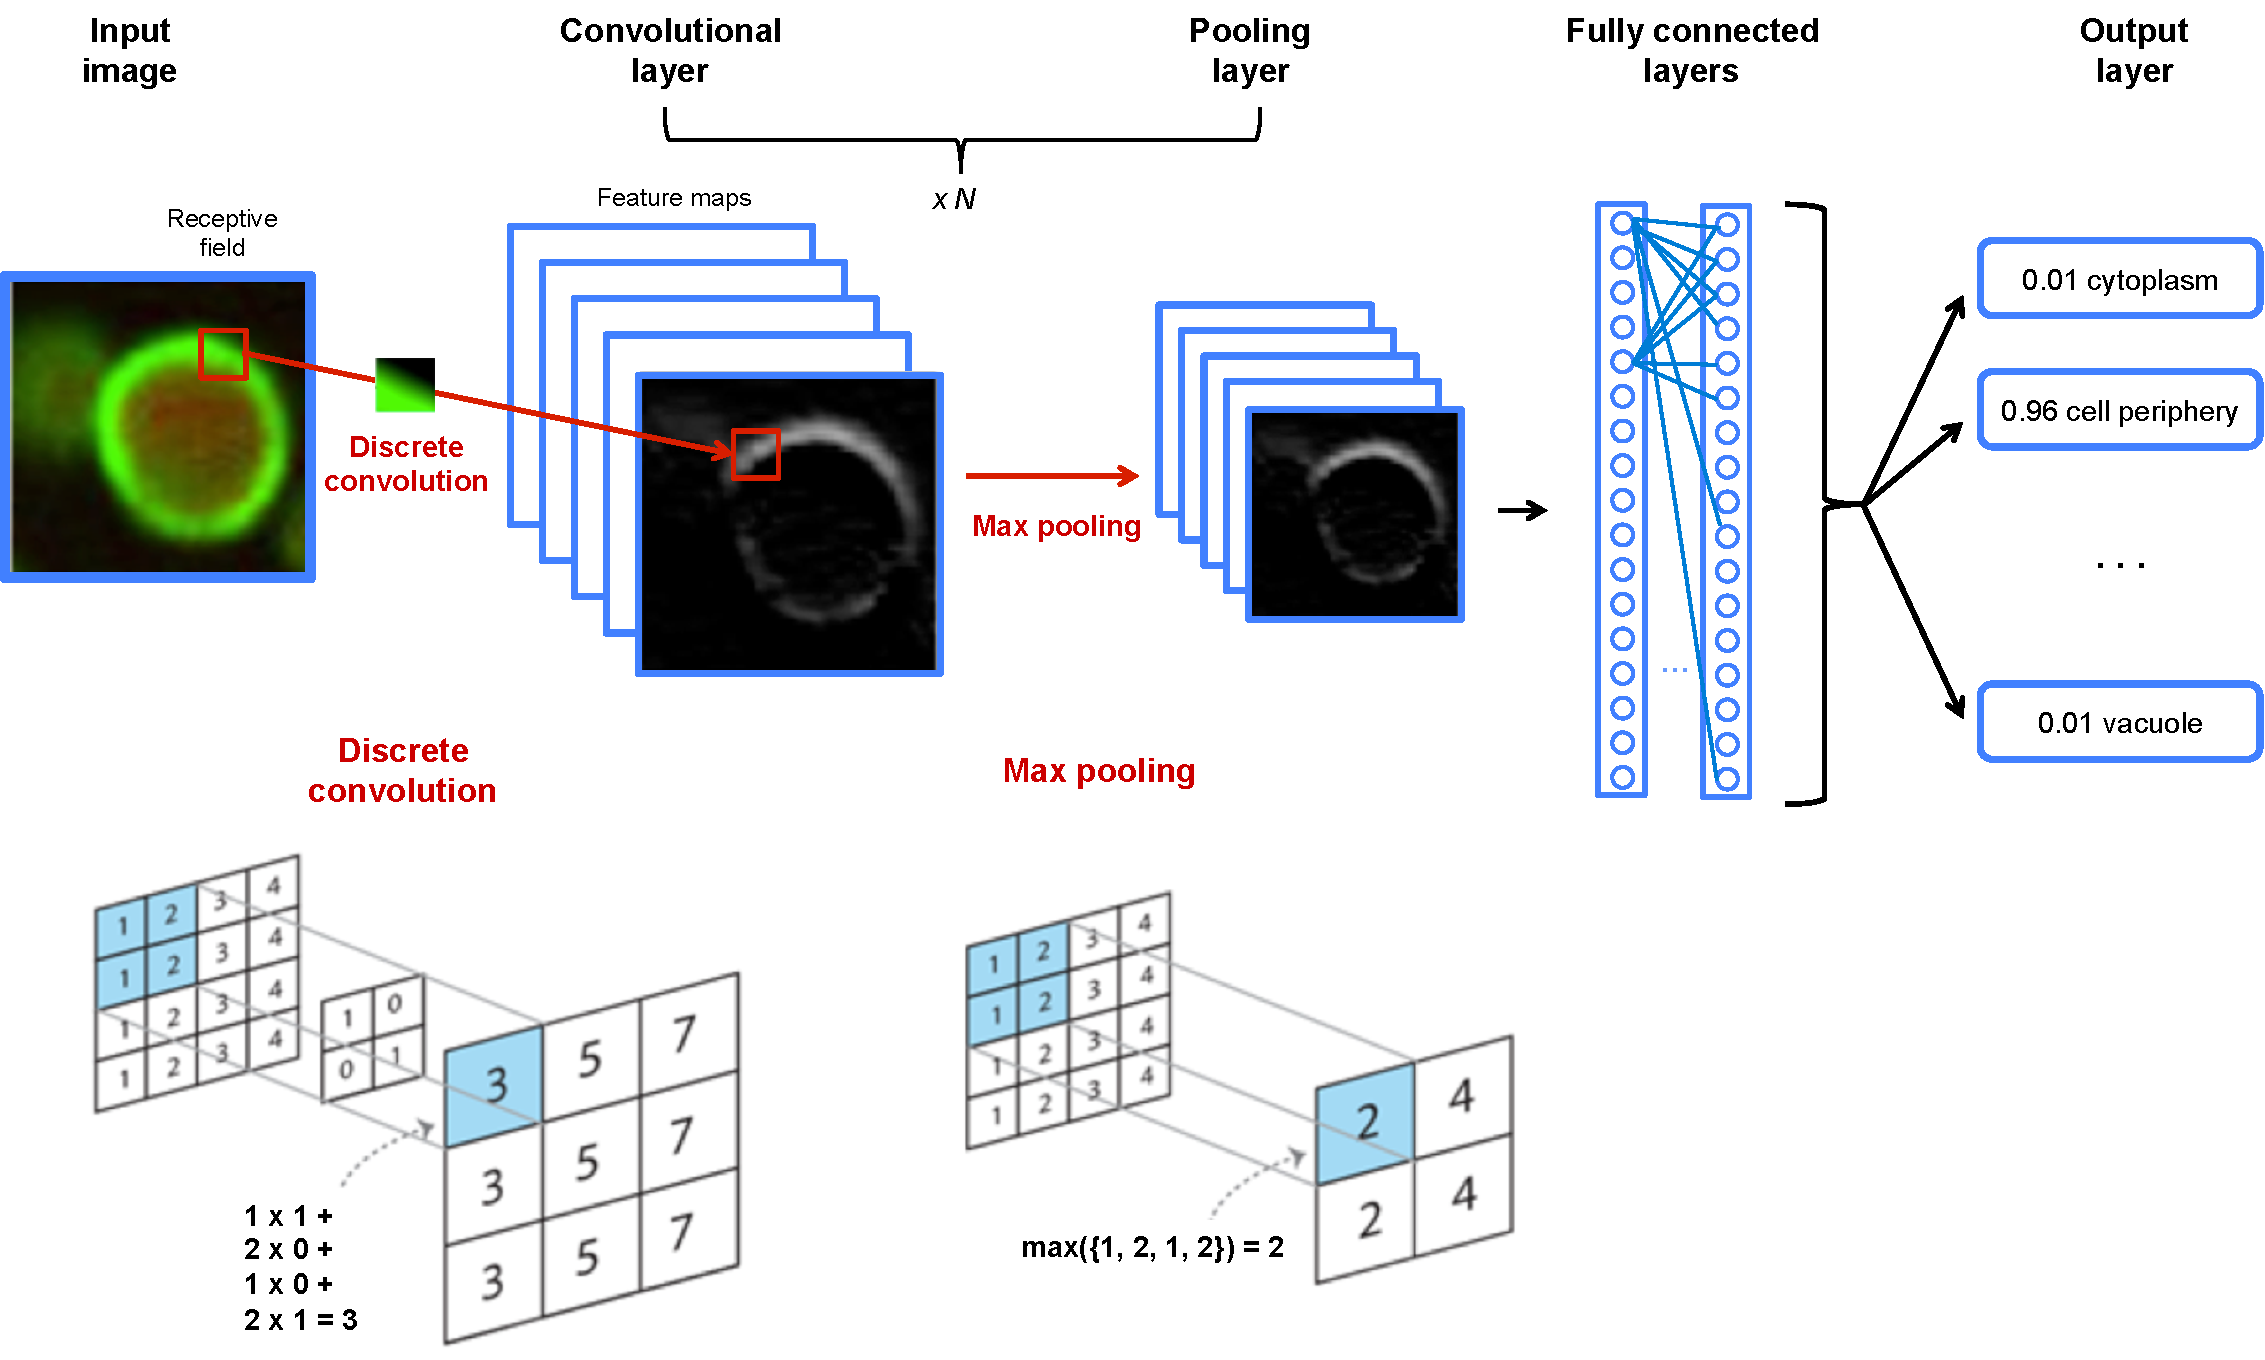
\includegraphics[width=1.0\textwidth]{cnn}
\caption[Convolutional neural network (CNN).]{Convolutional neural network (CNN). (a) A typical CNN consists of a number of convolutional and pooling layers, two fully connected layers, and one output layer. Each convolutional layer consists of multiple feature maps, with neurons responding to a particular feature in a receptive field (red square). One feature map responding to the membrane of a cell at a particular angle is highlighted on the edge. (b) Neuron activities result from a discrete convolution of their receptive field. (c) Max pooling computes the maximum neuron activity over a small patch, reducing the dimension of a convolutional layer.}
\label{fig:dl_cnn}
\end{figure}

A convolutional layer consists of multiple maps of neurons, so called feature maps or filters, with their size being equal to the dimension of the input image (\Cref{fig:dl_cnn}). Two concepts allow reducing the number of model parameters: local connectivity and parameter sharing. First, unlike in a fully connected network, each neuron within a feature map is only connected to a local patch of neurons in the previous layer, the so-called receptive field. Second, all neurons within a given feature map share the same parameters. Hence, all neurons within a feature map scan for the same feature in the previous layer, however at different locations. Different feature maps might, for example, detect edges of different orientation in an image, or sequence motifs in a genomic sequence. The activity of a neuron is obtained by computing a discrete convolution of its receptive field, i.e. computing the weighted sum of input neurons, and applying an activation function.

In most applications, the exact position and frequency of features is irrelevant for the final prediction, such as recognizing objects in an image. Using this assumption, the pooling layer summarizes adjacent neurons by computing, for example, the maximum or average over their activity, resulting in a smoother representation of feature activities. By applying the same pooling operation to small image patches that are shifted by more than one pixel, the input image is effectively down-sampled, thereby further reducing the number of model parameters.

A CNN typically consists of multiple convolutional and pooling layers, which allows learning more and more abstract features at increasing scales from small edges, to object parts, and finally entire objects. One or more fully connected layers can follow the last pooling layer. Model hyperparameters such as the number of convolutional layers, number of feature maps, or the size of receptive fields are application dependent and should be strictly selected on a validation data set (see below).


\subsection{Recurrent neural network} \label{sec:dl_rnn}

Recurrent neural networks (RNNs) are designed to model input sequences of variable length. They have been successfully applied to modelling long-range dependencies in natural text~\citep{sutskever_sequence_2014,bahdanau_neural_2014,xiong_dynamic_2016}, acoustic signals~\citep{deng_deep_2015,graves_speech_2013,hinton_deep_2012}, and biological sequences~\citep{agathocleous_protein_2010,sonderby_protein_2014,li_protein_2016,quang_danq:_2016}.  The input of a RNN is a sequence of vectors $x_1,\ldots,x_N$, such as the words of a sentence, nucleotides of a genomic sequence, or amino acids of a protein sequence. A RNN is called \emph{recurrent}, because it applies the same operation at every time step:
\begin{align}
  h_t=\textrm{sigmoid}(W_{hx}x_t+W_{hh}h_{t-1}+b_h)
\end{align}
$h_t$ is the hidden state vector of the RNN, which is sequentially updated based on the current input $x_t$ and the previous hidden state $h_{t-1}$. $h_t$ is also denoted as the \emph{memory} of the network, since it memorizes the input sequence $x_1,\ldots,x_t$ up to time step $t$. The last hidden state $h_T$ eventually memorises the entire input sequence. Importantly, the weights $W_{hx}$, $W_{hh}$, and $b_h$ are shared across time steps, which allows the network to process sequences of variable length. The output $y_t$ at time step $t$ is conditioned on the hidden state $h_t$, and thereby the entire past sequence:
\begin{align}
  y_t=f(W_{yh}+b_y)
\end{align}
$f$ is a task-specific activation function, such as the sigmoid function to model binary outputs or the softmax function to model categorical outputs. A RNN can either have a single output~$y_T$ at the end of the sequence, for example to predict the class of a protein, or it can have an output at every time step $t$, for example to predict the secondary structure for an entire protein sequence. The network parameters $\left\{W_{hx},W_{hh},b_h,W_{yh},b_y\right\}$ are trained similarly to a feedforward neural network by comparing model outputs $y_t$ with true output labels $y^\prime_t$ (\autoref{fig:dl_ann}), and by backpropagating the error signal back over time. RNNs have long been considered as hard to train, since an incorrect parameter initialization can lead to vanishing or exploding gradients. While exploding gradients can be controlled by clipping~\citep{pascanu_difficulty_2013}, vanishing gradients can be circumvented by the use of advanced RNN architectures, such as the long short-term memory (LSTM~\citep{hochreiter_long_1997}) or gated recurrent unit (GRU~\citep{chung_empirical_2014}) network. The core idea behind the LSTM and GRU is the use of additional gates to update the memory of the network only at certain time steps.

\begin{figure}[htbp!]
\centering
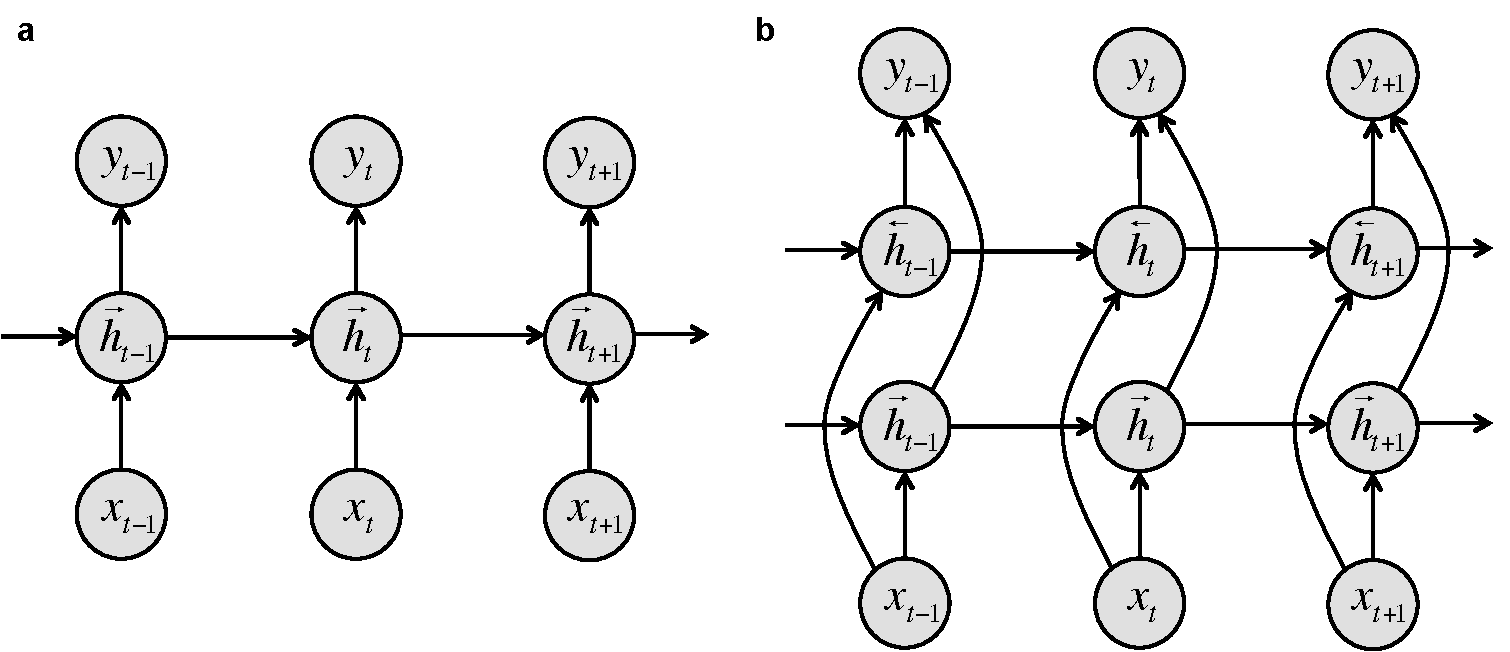
\includegraphics[width=1.0\textwidth]{rnn}
\caption[Recurrent neural network (RNN).]{Recurrent neural network (RNN). (a) A recurrent neural network scans an input sequence $x$ from left to right and updates at every time step $t$ its hidden state vector $h_t$ based on the previous hidden state $h_{t-1}$ and the current input $x_t$. Outputs $y_t$ are conditioned on $h_t$, which encodes the past sequence up to time step $t$. (b) A bidirectional RNN consists of a forward and backward RNN, which scan the input sequence in both directions. Outputs $y_t$ are conditioned on both the hidden state vector $\overrightarrow{h}_t$ of the forward RNN, and the hidden state vector $\overleftarrow{h}_t$ of the backward RNN, thereby on the entire sequence.}
\label{fig:rnn}
\end{figure}

The outputs $y_t$ of a RNN only depend on the past sequence, not the future sequence. In some applications, however, it is expedient to leverage information from the entire sequence. For example, the secondary structure of a protein sequence at position $t$ can depend on both amino acids to the left and to the right of $t$. A bidirectional RNN conditions its outputs $y_t$ on both the past and the future sequence. It consists of a forward and backward RNN, which scan the input sequence forward and backward, respectively, and concatenates their hidden state vectors:
\begin{align}
  \overrightarrow{h}_t&=\textrm{sigmoid}(\overrightarrow{W}_{hx}x_t+\overrightarrow{W}_{hh}h_{t-1}+\overrightarrow{b}_h) \\
  \overrightarrow{h}_t&=\textrm{sigmoid}(\overrightarrow{W}_{hx}x_t+\overrightarrow{W}_{hh}h_{t-1}+\overrightarrow{b}_h) \\
  h_t&=[\overrightarrow{h}_t, \overleftarrow{h}_t]
\end{align}
$\overrightarrow{h}_t$ and $\overleftarrow{h}_t$ is the hidden state vector at time step $t$ of the forward and backward RNN, which summarizes the input sequence before and after time step $t$, respectively. The concatenated hidden state vector $h_t$ summarizes both the past and future input sequence, and thereby conditions $y_t$ on the entire sequence.


\section{Deep learning for regulatory genomics} \label{sec:dl_genomics}

Conventional approaches for regulatory genomics relate sequence variation to changes in molecular traits. One approach is to leverage variation between genetically diverse individuals to map quantitative trait loci (QTL). This principle has been applied to identify regulatory variants that affect gene expression levels~\citep{montgomery_transcriptome_2010,pickrell_understanding_2010}, DNA methylation~\citep{bell_dna_2011,gibbs_abundant_2010}, histone marks~\citep{grubert_genetic_2015,waszak_population_2015}, and proteome variation~\citep{albert_genetics_2014,battle_genomic_2015,parts_heritability_2014,vincent_stacked_2010} (\Cref{fig:dl_genomics}~(a)). Better statistical methods have helped to increase the power to detect regulatory QTLs~\citep{kang_accurate_2008,parts_joint_2011,rakitsch_modelling_2016,stegle_bayesian_2010}, however any mapping approach is intrinsically limited to variation that is present in the training population. Thus, studying effects of rare mutations in particular requires extremely large datasets.

An alternative is to train models that use variation between regions within a genome (\Cref{fig:dl_genomics}~(a)). Splitting the sequence into windows centred on the trait of interest gives rise to tens of thousands of training examples for most molecular traits even when using a single individual. Even with large datasets, predicting molecular traits from DNA sequence is challenging due to multiple layers of abstraction between effect of individual DNA variants and the trait of interest, as well as the dependence of the molecular traits on a broad sequence context and interactions with distal regulatory elements.

The value of deep neural networks in this context is twofold. First, classical machine learning methods cannot operate on the sequence directly, and thus require predefining features that can be extracted from sequence based on prior knowledge (e.g. the presence of absence of single nucleotide variants (SNVs), k-mer frequencies, motif occurrences, conservation, known regulatory variants, or structural elements). Deep neural networks can help circumventing the manual extraction of features by learning them from data. Second, because of their representational richness, they can capture nonlinear dependencies in the sequence, interaction effects, and span wider sequence context at multiple genomic scales. Attesting to their utility, deep neural networks have been successfully applied to predict splicing activity~\citep{leung_deep_2014,xiong_human_2015}, specificities of DNA- and RNA binding proteins~\citep{alipanahi_predicting_2015}, or epigenetic marks and to study the effect of DNA sequence alterations~\citep{kelley_basset:_2016,zhou_predicting_2015}.

\begin{figure}[htbp!]
\centering
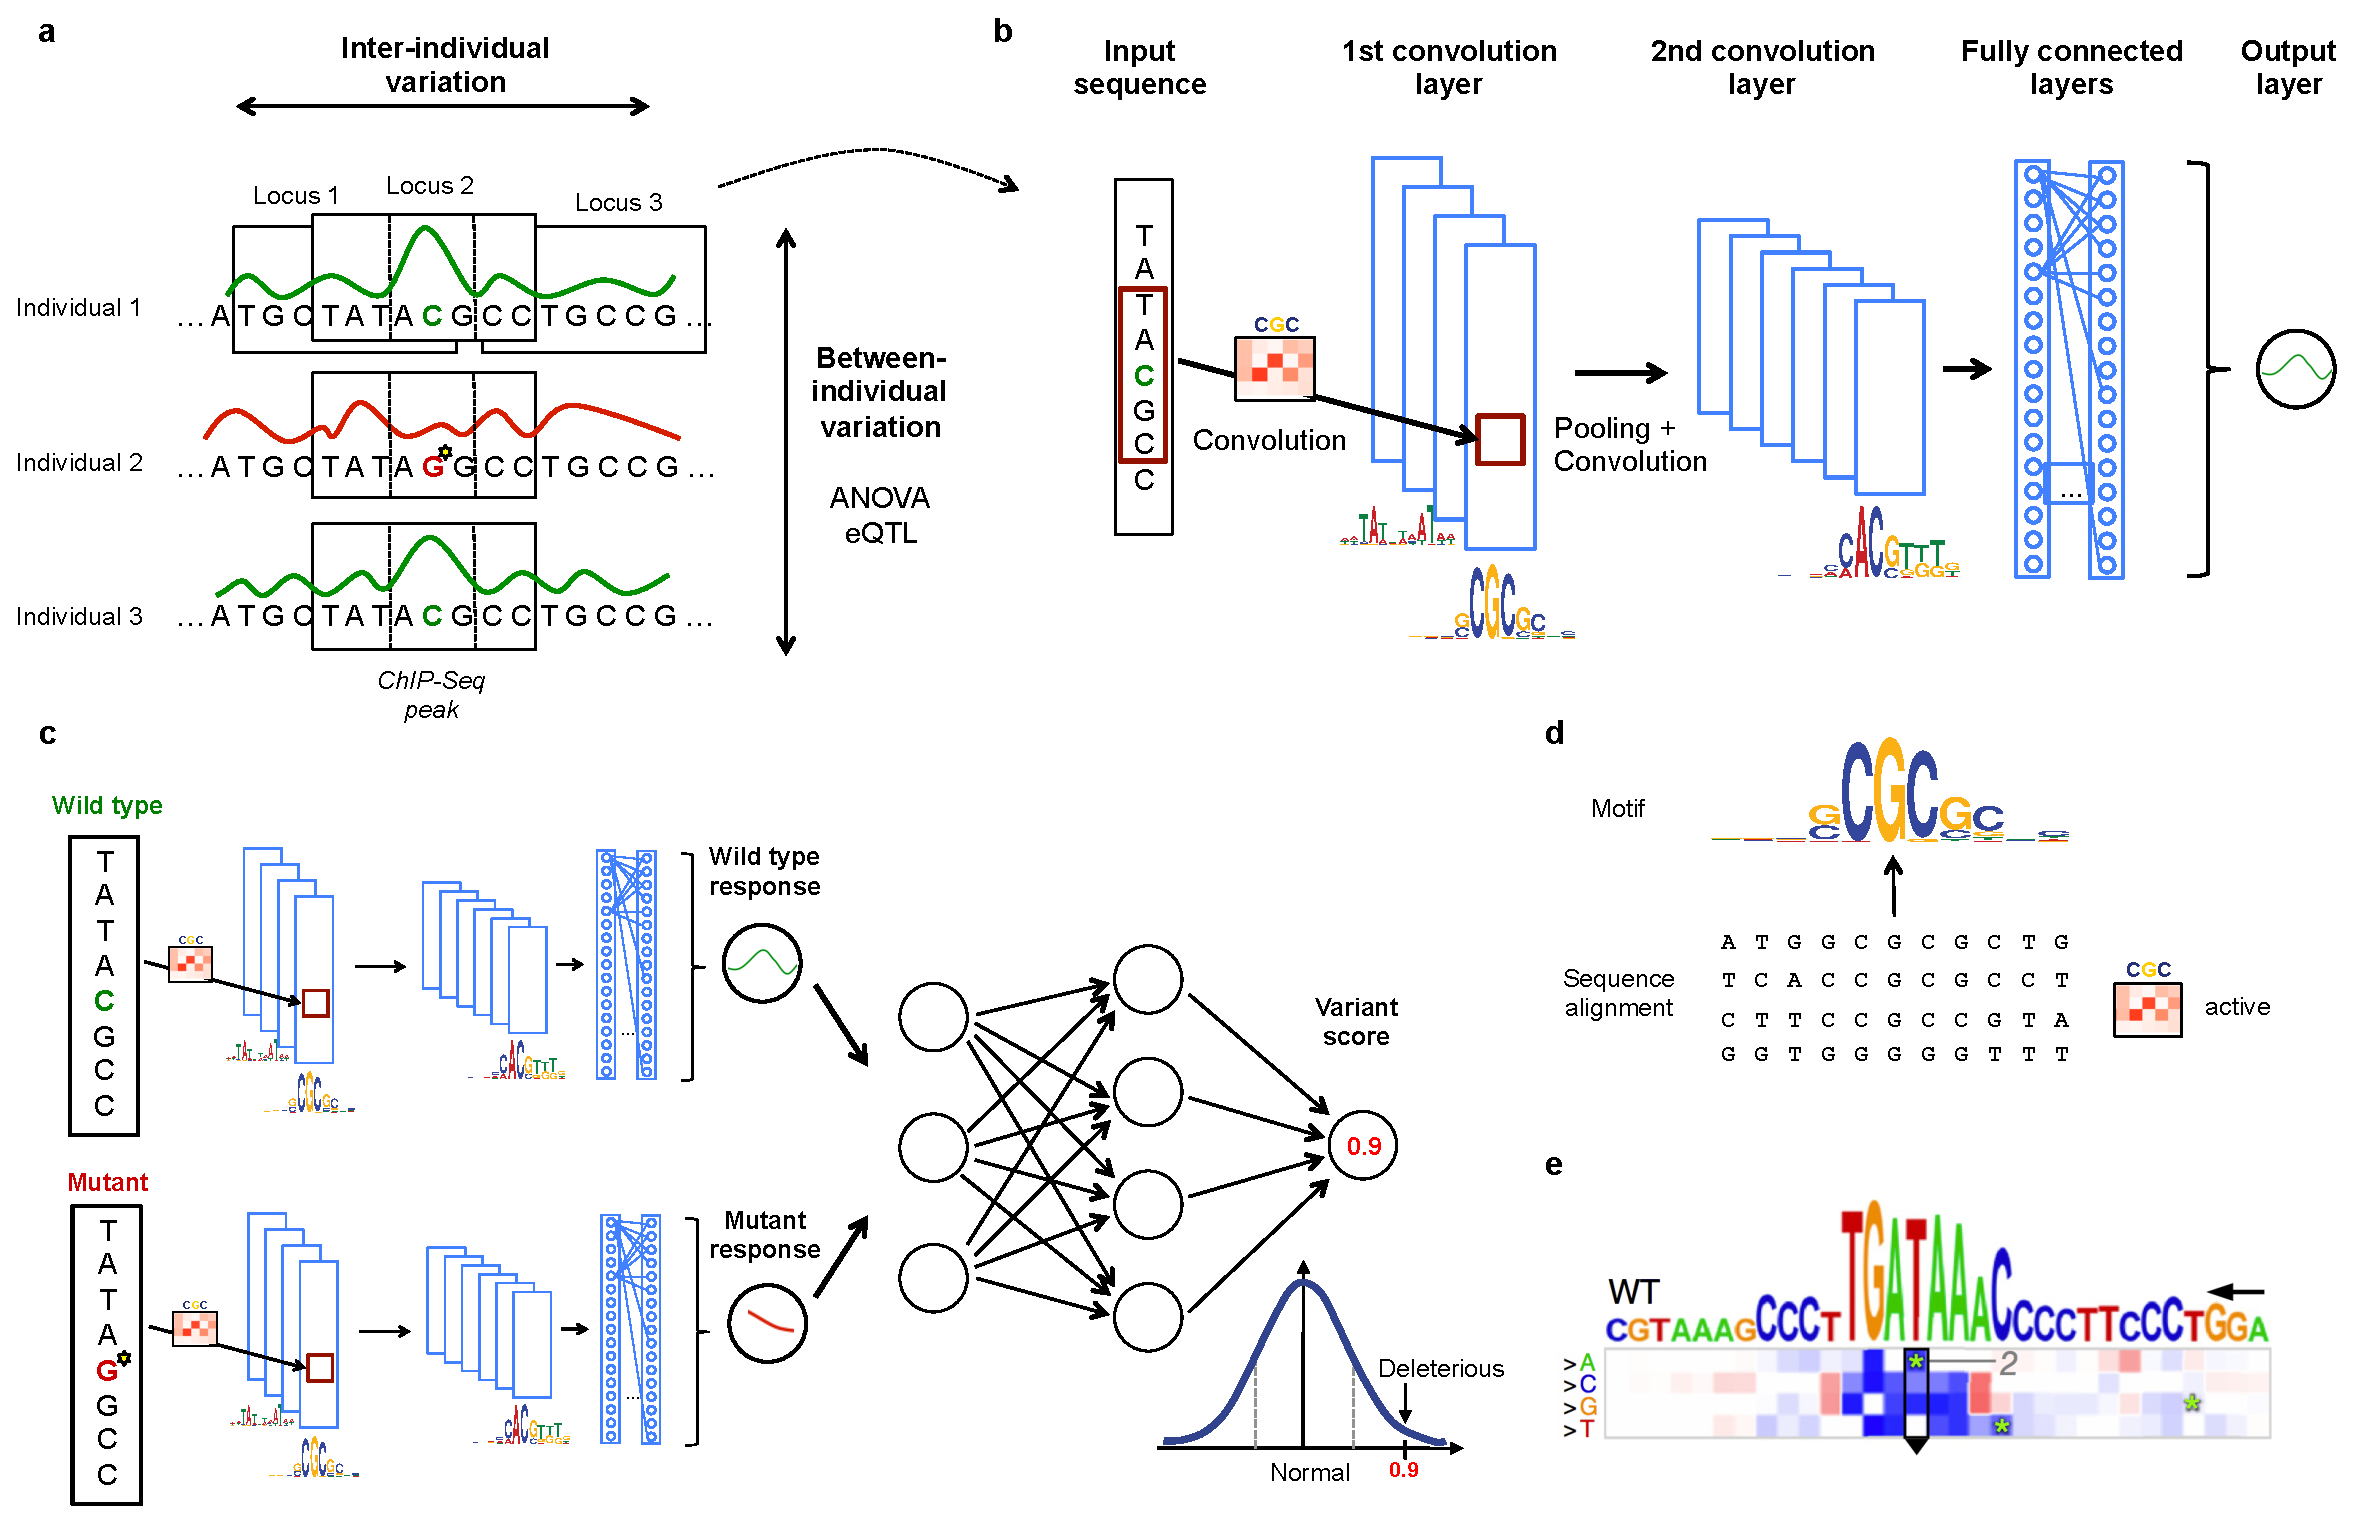
\includegraphics[width=1.0\textwidth]{genomics}
\caption[Principles of using neural networks for predicting molecular traits from DNA sequence.]{Principles of using neural networks for predicting molecular traits from DNA sequence. (a) DNA sequence and the molecular response variable along the genome for three individuals. Conventional approaches in regulatory genomics consider variations between individuals, whereas deep learning allows exploiting intra-individual variations by tiling the genome into sequence DNA windows centred on individual traits, resulting in large training datasets from a single sample. (b) One-dimensional convolutional neural network for predicting a molecular trait from the raw DNA sequence in a window. Filters of the first convolutional layer (example shown on the edge) scan for motifs in the input sequence. Subsequent pooling reduces the input dimension, and additional convolutional layers and can model interactions between motifs in the previous layer. (c) Response variable predicted by the neural network shown in (b) for a wild type and mutant sequence is used as input to an additional neural network that predicts a variant score and allows to discriminate normal from deleterious variants. (d) Visualization of a convolutional filter by aligning genetic sequences that maximally activate the filter and creating a sequence motif. (e) Mutation map of a sequence window. Rows correspond to the four possible base pair substitutions, columns to sequence positions. The predicted impact of any sequence change is colour coded. Letters on top denote the wild type sequence with the height of each nucleotide denoting the maximum effect across mutations (Figure panel adapted from \citet{alipanahi_predicting_2015}).}
\label{fig:dl_genomics}
\end{figure}


\subsection{Early applications of neural networks in regulatory genomics}

The first successful applications of neural networks in regulatory genomics replaced a classical machine learning approach with a deep model, without changing the input features. For example, \citet{xiong_human_2015} considered a fully connected feedforward neural network to predict the splicing activity of individual exons. The model was trained using more than 1000 pre-defined features extracted from the candidate exon and adjacent introns. Despite the relatively low number of 10700 training samples in combination with the model complexity, this method achieved substantially higher prediction accuracy of splicing activity compared to simpler approaches, and in particular was able to identify rare mutations implicated in splicing misregulation.


\subsection{Convolutional designs}

More recent work using convolutional neural networks (CNNs) allowed direct training on the DNA sequence, without the need to define features~\citep{alipanahi_predicting_2015,angermueller_accurate_2017,kelley_basset:_2016,zhou_predicting_2015}. The CNN architecture allows to greatly reduce the number of model parameters compared to a fully connected network by applying convolutional operations to only small regions of the input space and by sharing parameters between regions. The key advantage resulting from this approach is the ability to directly train the model on larger sequence windows (\Cref{sec:dl_cnn}; \Cref{fig:dl_genomics}~(b); \Cref{fig:dl_cnn}).

\citet{alipanahi_predicting_2015} considered convolutional network architectures to predict specificities of DNA- and RNA binding proteins. Their DeepBind model outperformed existing methods, was able to recover known and novel sequence motifs, and could quantify the effect of sequence alterations and identify functional SNVs. A key innovation that enabled training the model directly on the raw DNA sequence was the application of a one-dimensional convolutional layer. Intuitively, the neurons in the convolutional layer scan for motif sequences and combinations thereof, similar to conventional position-weight matrices~\citep{stormo_use_1982}. The learning signal from deeper layers informs the convolutional layer which motifs are most relevant. The motifs recovered by the model can then be visualized as heatmaps or sequence logos (\Cref{fig:dl_genomics}~(d)).


\subsection{In silico prediction of mutation effects}

An important application of deep neural networks trained on the raw DNA sequence is to predict the effect of mutations in silico. Such model-based assessments of the effect of sequence changes complement methods based on QTL mapping, and can in particular help to uncover regulatory effects of rare SNVs or to fine-map likely causal genes. An intuitive approach for visualizing such predicted regulatory effects are mutation maps~\citep{alipanahi_predicting_2015}, whereby the effect of all possible mutations for a given input sequence is represented in a matrix view (\Cref{fig:dl_genomics}~(e)). The authors could further reliably identify deleterious SNVs, by training an additional neural network with predicted binding scores for a wild type and mutant sequence (\Cref{fig:dl_genomics}~(c)).


\subsection{Joint prediction of multiple traits and further extensions}

Following their initial successes, convolutional architectures have been extended and applied to a range of tasks in regulatory genomics. For example, \citet{zhou_predicting_2015} considered these architectures to predict chromatin marks from DNA sequence. The authors observed that the size of the input sequence window is a major determinant of model performance, where larger windows (now up to 1~kbp) coupled with multiple  convolutional layers enabled capturing sequence features at different genomic length scales. A second innovation was to use neural network architectures with multiple output variables (so called multi-task neural networks), here to predict multiple chromatin states in parallel. Multi-task architectures allow learning shared features between outputs, thereby improving generalization performance, and markedly reducing the computational cost of model training compared to learning independent models for each trait~\citep{dahl_multi-task_2014}.

In a similar vein, \citet{kelley_basset:_2016} developed the open-source deep learning framework Basset, to predict DNase-I hypersensitivity across multiple cell types and to quantify the effect of SNVs on chromatin accessibility. Again, the model improved prediction performance compared to conventional methods and was able to retrieve both known and novel sequence motifs that are associated with DNase-I hypersensitivity. Most recently, \citet{koh_denoising_2017} applied CNNs to de-noise genome-wide chromatin immunoprecipitation followed by sequencing data in order to obtain a more accurate prevalence estimate for different chromatin marks.

At present, CNNs are among the most widely used architectures to extract features from fixed sized DNA sequence windows. However, alternative architectures could also be considered. For example, RNNs are suited to model sequential data~\citep{lipton_critical_2015}, and have been applied for modelling natural language and speech~\citep{che_distilling_2015,deng_deep_2015,graves_speech_2013,hinton_deep_2012,sutskever_sequence_2014,xiong_dynamic_2016}, protein sequences~\citep{agathocleous_protein_2010,sonderby_protein_2014}, clinical medical data~\citep{che_distilling_2015}, and to a limited extent DNA sequences~\citep{lee_dna-level_2015}. RNNs are appealing for applications in regulatory genomics, because they allow modelling sequences of variable length, and to capture long-range interactions within the sequence and across multiple outputs. However, at present, RNNs are more difficult to train than CNNs, and additional work is needed to better understand the settings where one should be preferred over the other.

Complementary to supervised methods, unsupervised deep learning architectures learn low-dimensional feature representations from high-dimensional unlabelled data, similarly to classical principal components analysis or factor analysis, but using a non-linear model. Examples of such approaches are stacked autoencoders~\citep{vincent_stacked_2010}, restricted Boltzmann machines, and deep belief networks~\citep{hinton_reducing_2006}. The learned features can be used to visualize data or as input for classical supervised learning tasks. For example, sparse autoencoders have been applied to classify cancer cases using gene-expression profiles~\citep{fakoor_using_2013}, or to predict protein backbones~\citep{lyons_predicting_2014-1}. Restricted Boltzmann machines can also be used for unsupervised pre-training of deep networks to subsequently train supervised models of protein secondary structures~\citep{spencer_deep_2015}, disordered protein regions~\citep{eickholt_predicting_2012,eickholt_dndisorder:_2013}, or amino-acid contacts~\citep{eickholt_predicting_2012}. Skip-gram neural networks have been applied to learn low-dimensional representations of protein sequences and improve protein classification~\citep{asgari_protvec:_2015}. In general, unsupervised models are a powerful approach if large quantities of unlabelled data are available to pre-train complex models. Once trained, these models can help to improve performance on classification tasks, for which smaller numbers of labelled examples are typically available.


\section{Deep learning for biological image analysis}

Historically, perhaps the most important successes of deep neural networks have been in image analysis. Deep architectures trained on millions of photographs can famously detect objects in pictures better than humans do~\citep{he_deep_2015}. All current state-of-the-art models in image classification, object detection, image retrieval, and semantic segmentation, make use of neural networks. The convolutional neural network (\Cref{sec:dl_cnn}) is the most common network architecture for image analysis. Briefly, a CNN performs pattern matching (convolution) and aggregation (pooling) operations. At a pixel level, the convolution operation scans the image with a given pattern, and calculates the strength of the match for every position. Pooling determines the presence of the pattern in a region, for example by calculating the maximum pattern match in smaller patches (max-pooling), thereby aggregating region information into a single number (\Cref{fig:dl_cnn}; \Cref{fig:dl_image_cnn}). The successive application of convolution and pooling operations is at the core of most network architectures used in image analysis.

\begin{figure}[htbp!]
\centering
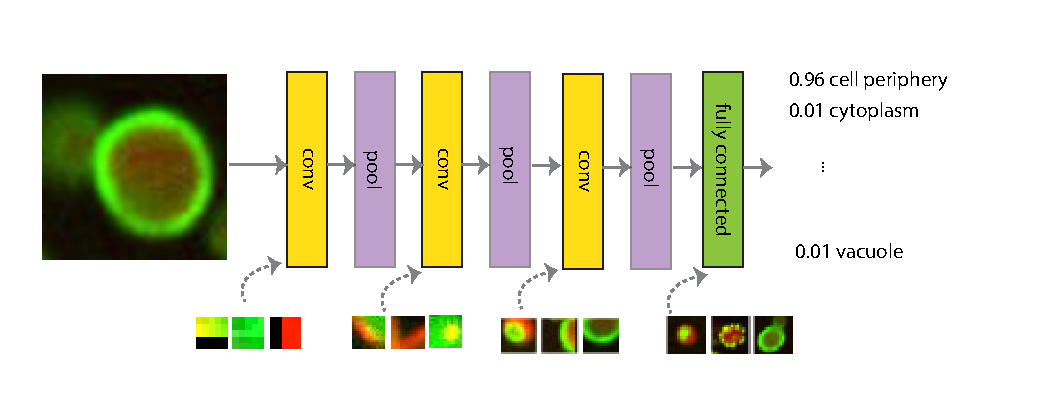
\includegraphics[width=1.0\textwidth]{image}
\caption[Deep neural network for image analysis.]{Convolution and pooling operators are stacked, thereby creating a deep network for image analysis. In standard applications, convolution layers are followed by a pooling layer (\Cref{sec:dl_cnn}). In this example, the lowest level convolutional units operate on 3x3 patches, but deeper ones use and capture information from larger regions. These convolutional pattern-matching layers are followed by one or multiple fully connected layers to learn which features are most informative for classification. For each layer with learnable weights, three example images that maximize some neuron output are shown.}
\label{fig:dl_image_cnn}
\end{figure}


\subsection{First applications in computational biology}

The early applications of deep networks for biological images focused on pixel level tasks, with additional models building on the network outputs. For example, \citet{ning_toward_2005} applied convolutional neural networks in a study that predicted abnormal development in C. elegans embryo images. They trained a CNN on 40x40 pixel patches to classify the centre pixel to cell wall, cytoplasm, nucleus membrane, nucleus, or outside medium, using three convolutional and pooling layers, followed by a fully connected output layer. The model predictions were then fed into an energy-based model for further analysis. CNNs have outperformed standard methods, e.g. Markov random fields and conditional random fields~\citep{li_markov_2009} in such raw data analysis tasks, for example restoring noisy neural circuitry images~\citep{jain_supervised_2007}.

Adding layers allows moving from clearing up pixel noise to modelling more abstract image features.~\citet{ciresan_mitosis_2013} used five convolutional and pooling layers, followed by two fully connected layers, to find mitosis in breast histology images. This model won the mitosis detection challenge at the International Conference of Pattern Recognition 2012, outperforming competitors by a substantial margin. The same approach was also used to segment neuronal structures in electron microscopy images, classifying each pixel as membrane or non-membrane~\citep{ciresan_deep_2012}. In these applications, while the CNNs were trained in an end-to-end manner, additional post-processing was required to obtain class probabilities from the outputs for new images.

Successive pooling operations lose information on localization, as only summaries are retained from larger and larger regions. To avoid this, skip links can be added to carry information from early, fine-grained layers forward to deeper ones. The currently best performing pixel level classification method for neuronal structures, U-Net~\citep{ronneberger_u-net:_2015}) employs an architecture in which neurons take inputs from lower layers to localize high resolution features, as well as to overcome the arbitrary choice of context size.


\subsection{Analysis of whole cells, cell populations, and tissues}

In many cases, pixel-level predictions are not required. For example, \citet{xu_deep_2014} classified colon histopathology images into cancerous and non-cancerous, finding that supervised feature learning with deep networks was superior to using hand-crafted features. \citet{parnamaa_accurate_2016} used CNNs to classify pre-segmented image patches of individual yeast cells carrying a fluorescent protein to different subcellular localization patterns. Again, deep networks outperformed methods based on traditional features. Further, \citet{kraus_classifying_2015} combined the segmentation and classification tasks into a single architecture that can be learned end-to-end, and applied the model to full resolution yeast microscopy images. This approach allowed classifying entire images without performing segmentation as a pre-processing step. CNNs have even been applied to count bacterial colonies in agar plates~\citep{ferrari_bacterial_2015}. Since the early de-noising applications on the pixel level, the field has been moving towards end-to-end image analysis pipelines that make use of large bioimage datasets, and the representational power of CNNs.


\subsection{Re-using trained models}

Training convolutional neural networks requires large datasets. While biological data acquisition can be expensive, this does not mean that deep neural networks cannot be used when millions of images are not available. Regardless of image source, lower levels of the network tend to capture similar signal (edges, blobs) that are not specific to the training data and the application, but instead recur in perceptual tasks in general. Thus, convolutional neural networks can re-use pictures from a similar domain to help with learning, or even be pre-trained on other data, thereby requiring fewer images to fine-tune the model for the task of interest. Indeed, \citet{donahue_decaf:_2013} showed that features learned from millions of images to classify objects, can successfully be used in image retrieval, detection or classification on new domains where only hundreds of images are labelled. The effectiveness of such an approach depends on the similarity between the training data and the new domain~\citep{ghahramani_how_2014}.

\begin{figure}[htbp!]
\centering
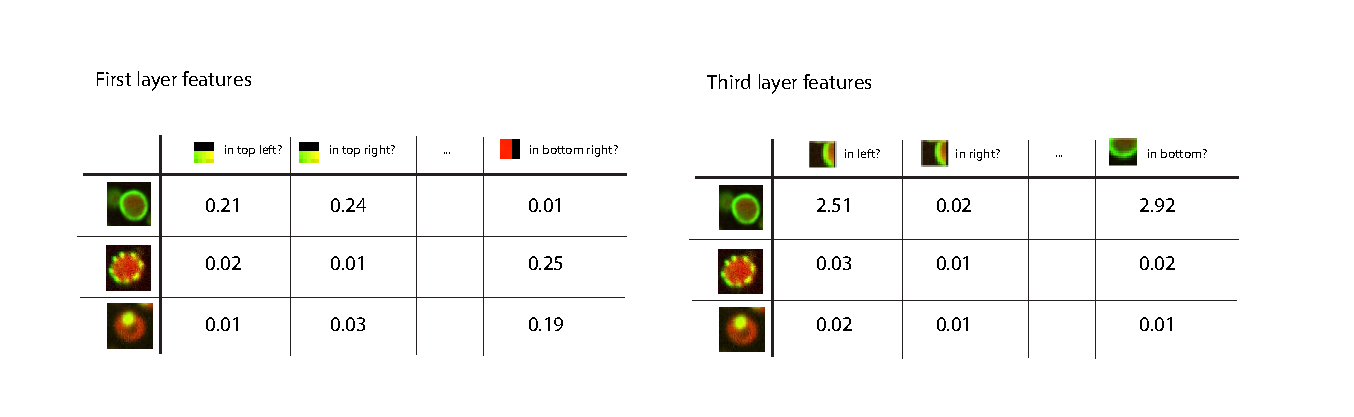
\includegraphics[width=1.0\textwidth]{image_pretrain}
\caption[Feature extraction with pre-trained convolutional neural networks.]{A pre-trained network can be used as a generic feature extractor. Feeding input into the first layer (left) gives a low-level feature representation in terms of patterns (left to right) present in smaller patches in every cell (top to bottom). Neuron activations extracted from deeper layers (right) give rise to more abstract features that capture information from a larger segment of the image.}
\label{fig:dl_image_pretrain}
\end{figure}

The concept of transferring model parameters has also been successful in bioimage analysis. For example, \citet{zhang_deep_2015} showed that features learned from natural images can be transferred to biological data, improving the prediction of Drosophila melanogaster developmental stages from in situ hybridization images. The model was first pre-trained on data from the ImageNet~\citep{russakovsky_imagenet_2015}, an open corpus of more than one million diverse images, to extract rich features at different scales. \citet{xie_beyond_2015} further used synthetic images to train a CNN for automatic cell counting in microscopy images. We expect that network repositories that host pre-trained models will emerge for biological image analysis; such efforts already exist for general image processing tasks (see learning section below). These trained models could be downloaded and used as feature extractors (\Cref{fig:dl_image_pretrain}), or further fine-tuned and adapted to a particular task on small-scale data.


\subsection{Interpreting and visualizing convolutional networks} \label{sec:dl_inter}
Convolutional neural networks have been successful across many domains. In interpreting their performance, it is useful to understand the features they capture.

\textit{Visualizing input weights.} One way to understand what a particular neuron represents is to look for inputs that maximally activate it. Under some mathematical constraints, these patterns are proportional to the incoming weights. \citet{krizhevsky_imagenet_2012} visualized weights in the first convolutional layer, and found that these maximally activating patterns correspond to colour blobs, edges at different orientations, and Gabor-like filters (\Cref{fig:dl_image_pretrain}). Gabor filters are widely used pre-defined features in image analysis; neural networks rediscover them in a data driven way as a useful component of the image model. Higher layer weights can be visualized as well, but as the inputs are not pixels, their weights are more difficult to interpret.

\textit{Finding images that maximize neuron activity.} To understand the deeper layers in terms of input pixels, \citet{girshick_rich_2014} and \citet{simonyan_deep_2013} generated images that maximize the output of individual neurons. While this approach yields no explicit representation, it can provide an overview of the type of features that differentiate images with large neuron activity from all others.  Such visualizations tend to show that second layer features combine edges from the first layer, thereby detecting corners and angles, deeper layer neurons activate for specific object parts (e.g. noses, eyes), and the deepest layers detect whole objects (e.g. faces, cars). It is complicated to hand-engineer features that look specifically for noses, eyes, or faces, but neural networks can learn these features solely from input-output examples.

\textit{Hiding important image parts.} To understand which image parts are important for determining the value of each feature, \citet{zeiler_visualizing_2014-1} occluded images with smaller grey boxes. The parts that are most influential will drastically change the feature value when occluded. In a similar vein, \citet{simonyan_deep_2013} and \citet{springenberg_striving_2014} visualised which individual pixels make the most difference in the feature, and \citet{bach_pixel-wise_2015} developed pixel relevance for individual classification decisions in a more general framework. This information can also be used for object localisation or segmentation, as the sensitive image pixels usually correctly correspond to the true object. \citet{kraus_classifying_2015} used this idea to effectively localize cells in large microscopy images.

\textit{Visualising similar inputs in two dimensions.} Visualising the CNN representations can help gauge what inputs get mapped to similar feature vectors, and hence understand what the model has learned. \citet{donahue_decaf:_2013} projected CNN features into two dimensions to show that each subsequent layer transforms data to be more and more separable by a linear classifier. In general, different CNN visualisation methods show that higher layer features are more specific to the learning task, while low-level features tend to capture general aspects of images, such as edges, corners, etc.


\section{Off-the-shelf tools and practical considerations}

\subsection{Deep learning frameworks}

Deep learning frameworks have been developed to easily build neural networks from existing modules on a high level. The most popular ones are Caffe~\citep{jia_caffe:_2014}, Theano~\citep{bastien_theano:_2012}, Torch7~\citep{collobert_torch7:_2011}, and TensorFlow~\citep{abadi_tensorflow:_2016} (\Cref{tab:dl_tools}), which differ in modularity, ease of use and the way models are defined and trained.

Caffe~\citep{jia_caffe:_2014} is developed by the Berkeley Vision and Learning Center and is written in C++. The network architecture is specified in a configuration file and models can be trained and used via command line, without writing code at all. Additionally, Python and MATLAB interfaces are available. Caffe offers one of the most efficient implementations for CNNs and provides multiple pre-trained models for image recognition, make it well suited for computer vision tasks. As a downside, custom models need to be implemented in C++, which can be difficult. Additionally, Caffe is not optimized for recurrent architectures.

Theano~\citep{bastien_theano:_2012} is developed and maintained by the University of Montreal and written in Python and C++. Model definitions follow a declarative instead of an imperative programing paradigm, which means that the user specifics what needs to be done, not in which order. A neural network is declared as a computational graph, which is then compiled to native code and executed. This design allows Theano to optimize computational steps and to automatically derive gradients—one of its main strengths. Consequently, Theano is well suited for building custom models and offers particularly efficient implementations for RNNs. Software wrappers such as Keras\footnote{\url{https://github.com/fchollet/keras}} or Lasagne\footnote{\url{https://github.com/Lasagne/Lasagne}} provide additional abstraction and allow building networks from existing components, and reuising pre-trained networks. The major drawback of Theano are frequently long compile times when building larger models.

\begin{table}
\centering
\begin{tabular}{p{2.5cm}|p{2.6cm}|p{2.6cm}|p{2.6cm}|p{2.6cm}}
\toprule
& \textbf{Caffee} & \textbf{Theano} & \textbf{Torch7} & \textbf{Tensorflow} \\
\hline
\textit{Core language} & C++ & Python, C++ & LuaJIT  & C++\\
\hline
\textit{Interfaces} & Python, Matlab & Python & C & Python, R \\
\hline
\textit{Wrappers} & & Lasagne, Keras, sklearn-theano & & Keras, Pretty Tensor, Scikit Flow \\
\hline
\textit{Programming paradigm} & Imperative & Declarative & Imperative & Declarative \\
\hline
\textit{Well suited for} & CNNs, Reusing existing models, Computer vision & Custom models, RNNs & Custom models, CNNs, Reusing existing models & Custom models, Parallelization, RNNs \\
\bottomrule
\end{tabular}
\caption{Overview of existing deep learning frameworks, comparing four widely used software solutions.}
\label{tab:dl_tools}
\end{table}

Torch7~\citep{collobert_torch7:_2011} was initially developed at the University of New York and is based on the scripting language LuaJIT. Networks can be easily built by stacking existing modules and are not compiled, hence making it more suited for fast prototyping than Theano. Torch7 offers an efficient CNN implementation and access to a range of pre-trained models. A possible downside is the need of the user to be familiar with the LuaJIT scripting language. Also, LuaJIT is less suited for building custom recurrent networks.

TensorFlow~\citep{abadi_tensorflow:_2016} is the most recent deep learning framework developed by Google. The software is written in C++ and offers interfaces to Python. Similar to Theano, a neural network is declared as a computational graph, which is optimized during compilation. However, the shorter compile time makes it more suited for prototyping. A key strength of TensorFlow is native support for parallelization across different devices, including central processing units (CPUs) and graphics processing units (GPUs), and compute nodes on a cluster. The accompanying tool TensorBoard allows to conveniently visualize networks in a web browser and to monitor training progress, e.g. learning curves or parameter updates. At present, TensorFlow provides the most efficient implementation for RNNs. The software is recent, and under active development, hence only few pre-trained models are currently available.


\subsection{Data preparation}

Training data are the key for every machine learning applications. Since more data with informative features usually result in better performance, effort should be spent on collecting, labelling, cleaning, and normalizing data.


\subsubsection{Required dataset sizes}

Most of the successful applications of deep learning have been in supervised learning settings, where sufficient labelled training samples are available to fit complex models. As a rule of thumb, the number of training samples should be at least as high as the number of model parameters, although special architectures and model regularization (see below) can help to avoid overfitting if training data are scarce~\citep{bengio_practical_2012}.

Central problems in regulatory genomics, e.g. predicting molecular traits from genotype, are limited in the number of training instances; hundreds to at most tens of thousands of training examples are typical. The strategy of considering a sequence windows centred on the trait of interest (e.g. splice site, transcription factor binding site, or epigenetic marks; \Cref{fig:dl_genomics}~(a)) is now a widely used approach and helps increasing the number of input-output pairs from a single individual.

In image analysis, data can be abundant, but manually curated and labelled training examples are typically difficult to obtain. In such instances, the training set can be augmented by scaling, rotating, or cropping the existing images, an approach that also enhances robustness~\citep{krizhevsky_imagenet_2012}. Another strategy is to reuse a network that was pre-trained on a large dataset for image recognition (e.g. AlexNet~\citep{krizhevsky_imagenet_2012}, VGG~\citep{simonyan_very_2014}, GoogleNet~\citep{szegedy_rethinking_2015}, or ResNet~\citep{he_deep_2015}), and to fine-tune its parameters on the data set of interest (e.g. microscopy images for a particular segmentation task). Such an approach exploits that different data sets share important characteristics and features, such as edges or curves, which can be transferred between them. Caffe, Lasagne, Torch, and to a limited extend TensorFlow provide repositories with pre-trained models.


\subsubsection{Partitioning data into training, validation, and test set} \label{sec:dl_eval}

Machine learning models need to be trained, selected, and tested on independent data sets to avoid over-fitting and assure that the model will generalize to unseen data. Holdout validation, partitioning the data into a training, validation, and test set, is the standard for deep neural networks (\Cref{fig:dl_tricks}~(c)). The training set is used to learn models with different hyperparameters, which are then assessed on the validation set. The model with best performance, e.g. prediction accuracy or mean squared error, is selected, and further evaluated on the test set to quantify the performance on unseen data and for comparison to other methods. Typical dataset proportions are 60\% for training, 10\% for validation, and 30\% for model testing. If the dataset is small, k-fold cross validation or bootstrapping can be used instead~\citep{hastie_elements_2005}.


\subsubsection{Normalization of raw data}

Appropriate choices for data normalization can help to accelerate training and the identification of a good local minimum.

Categorical features such as DNA nucleotides first need to be encoded numerically. They are typically represented as binary vectors with all but one entry set to zero, which indicates the category (one-hot coding). For example, DNA nucleotides (categories) are commonly encoded as A = (1 0 0 0), G = (0 1 0 0), C = (0 0 1 0), and T = (0 0 0 1) (\Cref{fig:dl_tricks}~(a)). A DNA sequence can then be represented as a binary string by concatenating the encoding nucleotides, and treating each nucleotide as an independent input feature of a feed forward neural network. In a CNN, the four bits of each encoded base are commonly considered analogously to colour channels of an image to preserve the entity of a nucleotide.

Numerical features are typically zero-centred by subtracting their mean value. Image pixels are usually not zero-centred individually, but jointly by subtracting the mean pixel intensity per colour channel~\citep{karpathy_cs231n_2016}. An additional common normalization step is to standardize features to unit variance. Whiting can be used to decorrelate features (\Cref{fig:dl_tricks}~(b)), but can be computationally involved, since it requires computing the feature covariance matrix~\citep{hastie_elements_2005}. If the distribution of features is skewed due to few extreme values, log transformations or similar processing steps may be appropriate. Validation and test data need to be normalized consistently with the training data. For example, features of the validation data need to be zero-centred by subtracting the mean computed on the training data, not on the validation data.

\begin{figure}[htbp!]
\centering
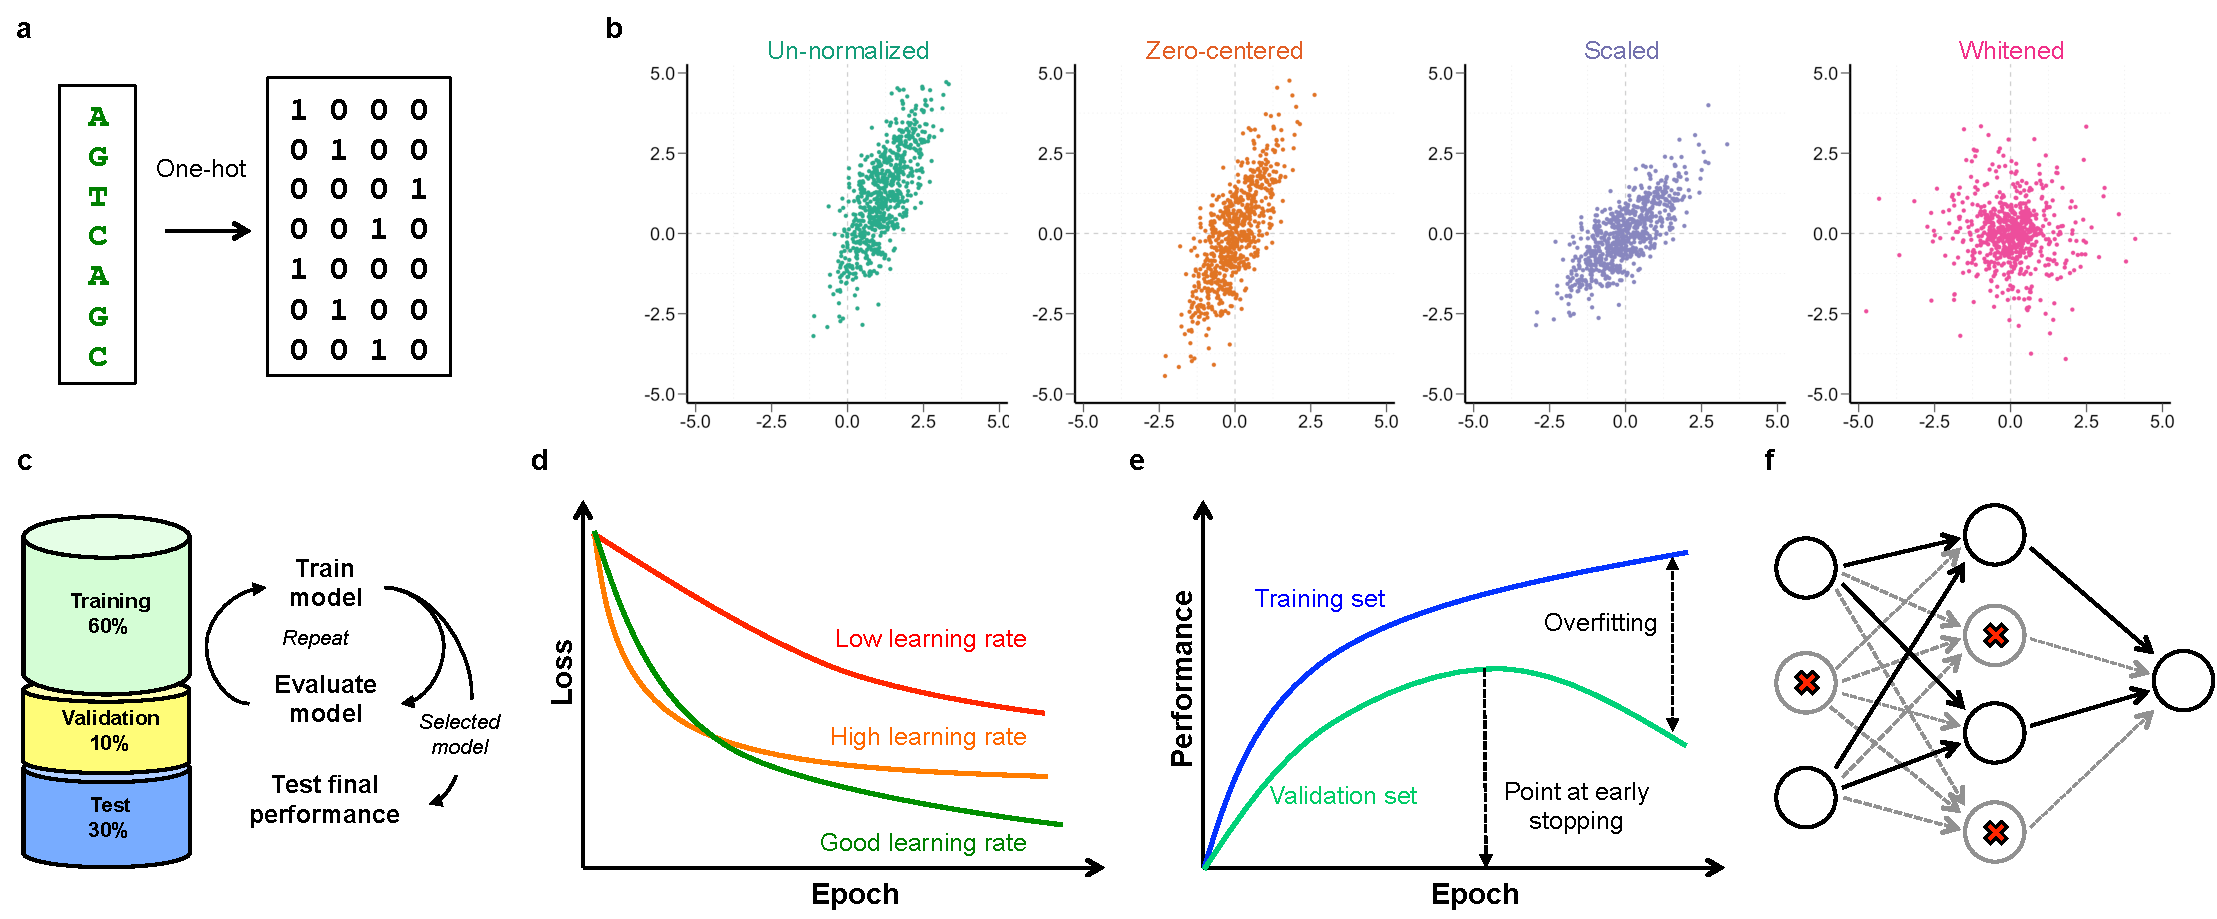
\includegraphics[width=1.0\textwidth]{tricks}
\caption[Data normalization and pre-processing for deep neural networks.]{Data normalization and pre-processing for deep neural networks. (a) DNA sequence one-hot encoded as binary vectors using codes A = 1 0 0 0, G = 0 1 0 0, C = 0 0 1 0, and T = 0 0 0 1. (b) Continuous data (green) after zero-centring (orange), scaling to unit variance (blue), and whiting (purple). (c) Holdout validation partitions the full data set randomly into training (${\approx}60\%$), validation (${\approx}10\%$) and test set (${\approx}30\%$). Models are trained with different hyperparameters on the training set, from which the model with the highest performance on the validation set is selected. The generalization performance of the model is assessed and compared with other machine learning methods on the test set. (d) The shape of the learning curve indicates if the learning rate is too low (red, shallow decay), too high (orange, steep decay followed by saturation), or appropriate for a particular learning task (green, gradual decay). (e) Large differences in the model performance on the training set (blue) and validation set (green) indicates overfitting. Stopping the training as soon as the validation set performance starts to drop (early stopping) can prevent overfitting. (f) Illustration of the dropout regularization. Shown is a feed forward neural network after randomly dropping out neurons (crossed out), which reduces the sensitivity of neurons to neurons in the previous layer due to non-existent inputs (greyed edges).}
\label{fig:dl_tricks}
\end{figure}


\subsection{Model building}

\subsubsection{Choice of model architecture}
After preparing the data, design choices about the model architectures need to be made. The default architecture is a feedforward neural network with fully connected hidden layers, which is an appropriate starting point for many problems. Convolutional architectures are well suited for multi- and high-dimensional data, such as two-dimensional images or abundant genomic data. Recurrent neural networks can capture long-range dependencies in sequential data of varying lengths, such as text, protein, or DNA sequences. More sophisticated models can be built by combining different architectures. To describe the content of an image, for example, a CNN can be combined with an RNN, where the CNN encodes the image and the RNN generates the corresponding image description~\citep{vinyals_show_2015,xu_ask_2015}. Most deep learning frameworks provide modules for different architectures and their combinations.

\subsubsection{Determining the number of neurons in a network}
The optimal number of hidden layers and hidden units is problem dependent and should be optimized on a validation set. One common heuristic is to maximize the number of layers and units without overfitting the data. More layers and units increase the number of representable functions and local optima, and empirical evidence show that it makes finding a good local optimum less sensitive to weight initialization~\citep{dauphin_identifying_2014}.


\subsubsection{Model training}
The goal of model training is to find parameters $w$ that minimize an objective function $L(w)$, which measures the fit between the predictions the model parameterized by $w$ and the actual observations. The most common objective functions are the cross-entropy for classification and mean-squared error for regression. Minimizing $L(w)$ is challenging since it is high-dimensional and non-convex (\Cref{fig:dl_tricks}; \Cref{fig:dl_ann}).

\subsubsection{Stochastic Gradient Descent}
Stochastic gradient descent is widely used to train deep models. Starting from an initial set of parameters $w_0$, the gradient $\Delta w$ of $L$ with respect to $w$ is computed for a random batch of only few, e.g. 128, training samples. $\Delta w$ points to the direction of steepest descent, towards which w is updated with step size eta, the learning rate (\Cref{fig:dl_ann}~(c)). At each step, the parameters are updated into the direction of steepest descent until a minimum is reached, analogously to a ball running down a hill to a valley~\citep{bengio_practical_2012}. The training performance strongly depends on parameter initialization, learning rate, and batch size.

\subsubsection{Parameter initialization}
In general, model parameters should be initialized randomly to avoid local optima determined by a fixed initialization. Starting points for model parameters can be sampled independently from a normal distribution with small variance, or more commonly from a normal distribution with its variance scaled inversely by the number of hidden units in the input layer~\citep{glorot_understanding_2010,he_delving_2015}.

\subsubsection{Learning rate and batch size}
The learning rate and batch size of stochastic gradient descent need to be chosen with care, since they can strongly impact training speed and model performance. Different learning rates are usually explored on a logarithmic scale such as 0.1, 0.01, or 0.001, with 0.01 as recommended default value~\citep{bengio_practical_2012}. A batch size of 128 training samples is suitable for most applications. The batch size can be increased to speed up training, or decreased to reduce memory usage, which can be important for training complex models on memory-limited GPUs. The optimum learning rate and batch size are connected, with larger batch sizes typically requiring smaller learning rates.

\subsubsection{Learning rate decay}
The learning rate can be gradually reduced during training, which is based on the idea that larger steps may be helpful in early training stages in order to overcome possible local optima, whereas smaller step sizes allowing exploring narrow parameter regions of the loss function in advanced stages of training. Common approaches include to linearly reduce the learning rate by a constant factor such as 0.5 after the validation loss stops improving, or exponentially after every training iteration or epoch~\citep{bengio_practical_2012,gawehn_deep_2016}.

\subsubsection{Momentum}
Vanilla stochastic gradient descent can be extended by `momentum', which usually improves training~\citep{sutskever_training_2013}. Instead of updating the current parameter vector $w_t$ at time $t$ by the gradient vector $\Delta w_{t+1}$ directly, a fraction of the previous update is added to the current one. With momentum rate $\nu$, weights are updated by a momentum vector  This approach can help to take larger steps in directions where gradients point consistently, and therefore speed up the convergence. The momentum rate $\nu$ can be set between $[0;1]$, and a typical value is $0.9$. Nesterov momentum~\citep{nesterov_method_1983,nesterov_introductory_2013} is a special form of the same concept, which sometimes provides additional advantages.

\subsubsection{Per-parameter adaptive learning rate methods} \label{sec:dl_adapt}
To reduce the sensitivity to the specific choice of the learning rate, adaptive learning rate methods, such as RMSprop, Adagrad~\citep{duchi_adaptive_2011}, and Adam~\citep{kingma_adam:_2014}, have been developed that one appropriately adapt the learning rate per parameter during. The most recent method, Adam, combines the strengths of previous methods RMSprop and Adagrad, and is generally recommended for many applications.

\subsubsection{Batch normalization}
Batch normalization~\citep{ioffe_batch_2015} is a recently described approach to reduce the dependency of training to the parameter initialization, speed up training, and reduce overfitting. It is easy to implement, has marginal additional compute costs, and has hence become common practice. Batch normalization zero centres and normalizes data not only at the input layer, but also at hidden layers before the activation function. This approach allows using higher learning rates and hence also accelerates training.

\subsubsection{Analyzing the learning curve}
To validate the learning process, the loss should be monitored as a function of the number of training epochs, i.e. the number times the full training set has been traversed (\Cref{fig:dl_tricks}~(d)). If the learning curve decreases slowly, the learning rate may be too small and should be increased. If the loss decreases steeply at the beginning but saturates quickly, the learning rate may to too high. Extreme learning rates can result in an increasing or fluctuating learning curve~\citep{bengio_practical_2012,karpathy_cs231n_2016}.

\subsubsection{Monitoring training and validation performance}
In parallel to the training loss, it is recommended to monitor the target performance such as the accuracy for both the training and validation set during training (\Cref{fig:dl_tricks}~(e)). A low or decreasing validation performance relative to the training performance indicates overfitting~\citep{bengio_practical_2012,karpathy_cs231n_2016}.

\subsubsection{Avoiding overfitting} \label{sec:dl_overfit}
Deep neural networks are notoriously difficult to train, and overfitting to data is a major challenge, since they are non-linear and have many parameters. Overfitting results from a too complex model relative to the size of the training set, and can thus be reduced by decreasing the model complexity, e.g. the number of hidden layers and units, or by increasing the size of the training set, e.g. via data augmentation (see above). The following training guidelines can help to avoid overfitting.

Dropout~\citep{srivastava_dropout:_2014} is the most common regularization technique and often one of the key ingredients to train deep models. Here, the activation of some neurons is randomly set to zero (`dropped out') during training in each forward pass, which intuitively results in an ensemble of different networks whose predictions are averaged (\Cref{fig:dl_tricks}~(e)). The dropout rate corresponds to the probability that a neuron is dropped out, where 0.5 is a sensible default value. In addition to dropping out hidden units, input units can be dropped, however usually at a lower rate. Dropout is often combined with regularizing the magnitude or parameter values by the L2 norm, and less commonly the L1 norm.

Another popular regularization method is `early stopping'. Here, training is stopped as soon as the validation performance starts to saturate or deteriorate, and the parameters with the best performance on the validation set chosen.

Layer-wise pre-training~\citep{bengio_greedy_2007,salakhutdinov_efficient_2012} should be considered if the model overfits despite the mentioned regularization techniques. Instead of training the entire network at once, layers are first pre-trained unsupervised using autoencoders or restricted Boltzmann machines. Afterwards, the entire network is fine-tuned using the actual supervised learning objective.

\subsubsection{Hyperparameter optimization} \label{sec:dl_hyper}
\Cref{tab:dl_params} summarizes recommendations and starting points for the most common hyperparameters, excluding architecture dependent hyperparameters such as the size and number of filters of a CNN. Since the best hyperparameter configuration is data and application dependent, models with different configurations should be trained and their performance be evaluated on a validation set. As the number of configurations grows exponentially with the number of hyperparameters, trying all of them is impossible in practice~\citep{bengio_practical_2012}. It is therefore recommended to optimize the most important hyperparameters such as the learning rate, batch size, or length of convolutional filters independently via line search, i.e. trying different values while keeping all other hyperparameters constant. The refined hyperparameter space can then be further explored by random sampling, and settings with the best performance on the validation set are chosen. Frameworks such as Spearmint~\citep{snoek_practical_2012}, Hyperopt~\citep{bergstra_hyperparameter_2013}, or SMAC~\citep{hutter_sequential_2011} allow to automatically explore the hyperparameter space using Bayesian optimization. However, although conceptually more powerful, they are at present more difficult to apply and parallelize than random sampling.

\subsubsection{Training on GPUs}
Training neural networks is more time consuming compared to shallow models, and can take hours, days, or even weeks, depending on the size of training set and model architecture. Training on GPUs can considerably reduce the training time (commonly by ten fold or more) and is therefore crucial for evaluating multiple models efficiently. The reason for this speedup is that learning deep networks requires large numbers of matrix multiplications, which can be parallelized efficiently on GPUs. All state of the art deep learning frameworks provide support to train models on either CPUs or GPUs without requiring any knowledge about GPU programming. On desktop machines, the local GPU card can often be used if the framework supports the specific brand. Alternatively, commercial providers provide GPU cloud compute clusters.

\subsubsection{Pitfalls}
No single method is universally applicable, and the choice of whether and how to use deep learning approaches will be problem specific. Conventional analysis approaches will remain valid and have advantages when data are scarce or if the aim is to assess statistical significance, which is currently difficult using deep learning methods. Another limitation of deep learning is the increased training complexity, which applies both to model design and the required compute environment.

\begin{table}
\centering
\begin{tabular}{p{4cm}|p{5cm}|p{4cm}}
\textbf{Name} & \textbf{Range} & \textbf{Default value} \\
\toprule
Learning rate & 0.1, 0.01, 0.001, 0.0001 & 0.01 \\
Batch size & 64, 128, 256 & 128 \\
Momentum rate & 0.8, 0.9, 0.95 & 0.9 \\
Weight initialization & Normal, Uniform, Glorot uniform & Glorot uniform \\
Per-parameter adaptive learning rate methods & RMSprop, Adagrad, Adadelta, Adam & Adam \\
Batch normalization & yes, no & yes \\
Learning rate decay & None, linear, exponential & Linear (rate 0.5) \\
Activation function & Sigmoid, Tanh, ReLU, Softmax & ReLU \\
Dropout rate & 0.1, 0.25, 0.5, 0.75 & 0.5 \\
l1, l2 regularization & 0, 0.01, 0.001 & \\
\bottomrule
\end{tabular}
\caption{Central parameters of a neural network and recommended settings.}
\label{tab:dl_params}
\end{table}


\section{Discussion}

Deep learning methods are a powerful complement to classical machine learning tools and other analysis strategies. Already, these approaches have found use in a number of applications in computational biology, including regulatory genomics and image analysis. The first publicly available software frameworks have helped to reduce the overhead of model development, and provided a rich, accessible toolbox to practitioners. We expect that continued improvement of software infrastructure will make deep learning applicable to a growing range of biological problems.

%!TEX root = ../thesis.tex
%*******************************************************************************
%****************************** Third Chapter **********************************
%*******************************************************************************
\chapter{Protocols and analysis of single-cell DNA methylation data} \label{sec:pro}

% **************************** Define Graphics Path **************************
\ifpdf
    \graphicspath{{Chapter3/Figs/Raster/}{Chapter3/Figs/PDF/}{Chapter3/Figs/}}
\else
    \graphicspath{{Chapter3/Figs/Vector/}{Chapter3/Figs/}}
\fi

Our undestanding of DNA methylation has been revolutionized by the development of BS-seq, which offers single-cytosine resolution and absolute quantification of 5mC genome-wide. Recent advances have demonstrated the power of single-cell sequencing to deconvolve mixed cell populations~\citep{jain_supervised_2007,deng_single-cell_2014,macaulay_single_2014}. Incorporating epigenetic information into this single-cell arsenal will provide insights into epigenetic heterogeneity and transform our understanding of gene regulation.

In the first section of this chapter, we will describe the scBS-seq protocol for genome-wide profiling of DNA methylation in single cells, a statistical method for quantifying methylation variability between cells, and applications to mouse ESCs. The work is based on \citet{smallwood_single-cell_2014}, which was joint work of Sebastien Smallwood, Heather Lee, Christof Angermueller, Felix Krueger, Heba Saadeh, Julian Peat, Simon Andrews, Oliver Stegle, and Wolf Reik.

\begin{center}
\begin{minipage}{.9\linewidth}
\underline{Individual contributions}: Sebastien Smallwood and Heather Lee designed the study, prepared scBS-seq libraries, analysed data and wrote the manuscript. Felix Krueger, Heba Saadeh, and Sebastien Smallwood performed sequence mapping and analysed data. Julian Peat contributed to technical developments. Christof Angermueller and Oliver Stegle analysed the data.
\end{minipage}
\end{center}

In the second section, we will describe the scM\&T-seq protocol for parallel profiling of DNA methylation and gene expression in single cells, methods for quantifying associations between DNA methylation and gene expression, and applications to mouse ESCs. The work is based on \citet{angermueller_parallel_2016}, which was joint work of Christof Angermueller, Stephen Clark, Heather Lee, Iain Macaulay, Mabel Teng, Tim Xiaoming Hu, Felix Krueger, Sebastien Smallwood, Chris Ponting, Thierry Voet, Gavin Kelsey, Oliver Stegle, and Wolf Reik.

\begin{center}
\begin{minipage}{.9\linewidth}
\underline{Individual contributions}: Christof Angermueller performed all statistical analyses of the data. Heather Lee, Iain Macaulay, Stephen Clark, and Sebastien Smallwood developed the protocol and performed experiments. Heather Lee, Iain Macaulay, Christof Angermueller, Stephen Clark, Oliver Stegle, Wolf Reik, and Chris Ponting interpreted the results. Mabel Teng contributed to method development. Tim Xiaoming Hu processed RNA-seq data. Felix Krueger processed BS-seq data. Wolf Reik, Gavin Kelsey, Iain Macaula, and Thierry Voet contributed protocols and reagents. Heather Lee, Iain Macaulay, Wolf Reik, and Thierry Voet conceived the project.
\end{minipage}
\end{center}

\section{Estimating DNA methylation variability in embryonic stem cells} \label{sec:bs}

\ifpdf
    \graphicspath{{Chapter3/bs/Figs/Raster/}{Chapter3/bs/Figs/PDF/}{Chapter3/bs/Figs/}}
\else
    \graphicspath{{Chapter3/bs/Figs/Vector/}{Chapter3/bs/Figs/}}
\fi

Several protocols have been developed for profiling average DNA methylation levels of in bulk populations of cells (\Cref{sec:intro_proto}). However, bulk profiling protocols are unable to directly estimate methylation heterogeneity between single cells, which is critical for studying embryonic development, cancer progression, and pluripotent stem cells. In the following, we will describe scBS-seq, an accurate and reproducible method for profiling DNA methylation in single cells, and a statistical model for estimating methylation heterogeneity in cell populations across the entire genome.


\subsection{Single-cell bisulfite sequencing protocol} \label{sec:bs_proto}

In commonly used BS-seq protocols, sequencing adaptors are ligated to fragmented DNA before bisulfite conversion, which results in a loss of information owing to DNA degradation by the bisulfite treatment. To minimize DNA loss from single cells, we developed a modification of post-bisulfite adaptor tagging~\citep{miura_amplification-free_2012-1}. In scBS-seq, bisulfite treatment is performed first, which results in simultaneous DNA fragmentation and conversion of unmethylated cytosines to thymine (\Cref{fig:bs_proto}). Then, synthesis of complementary strands is primed using oligonuleotides containing Illumina adaptor sequences and a 3' stretch of nine random nucleotides. This step is performed five times to maximize the number of tagged DNA strands and to generate multiple copies of each fragment. After capturing the tagged strands, a second adaptor is similarly integrated, and PCR amplification is performed with indexed primers.

\begin{figure}[htbp!]
\centering
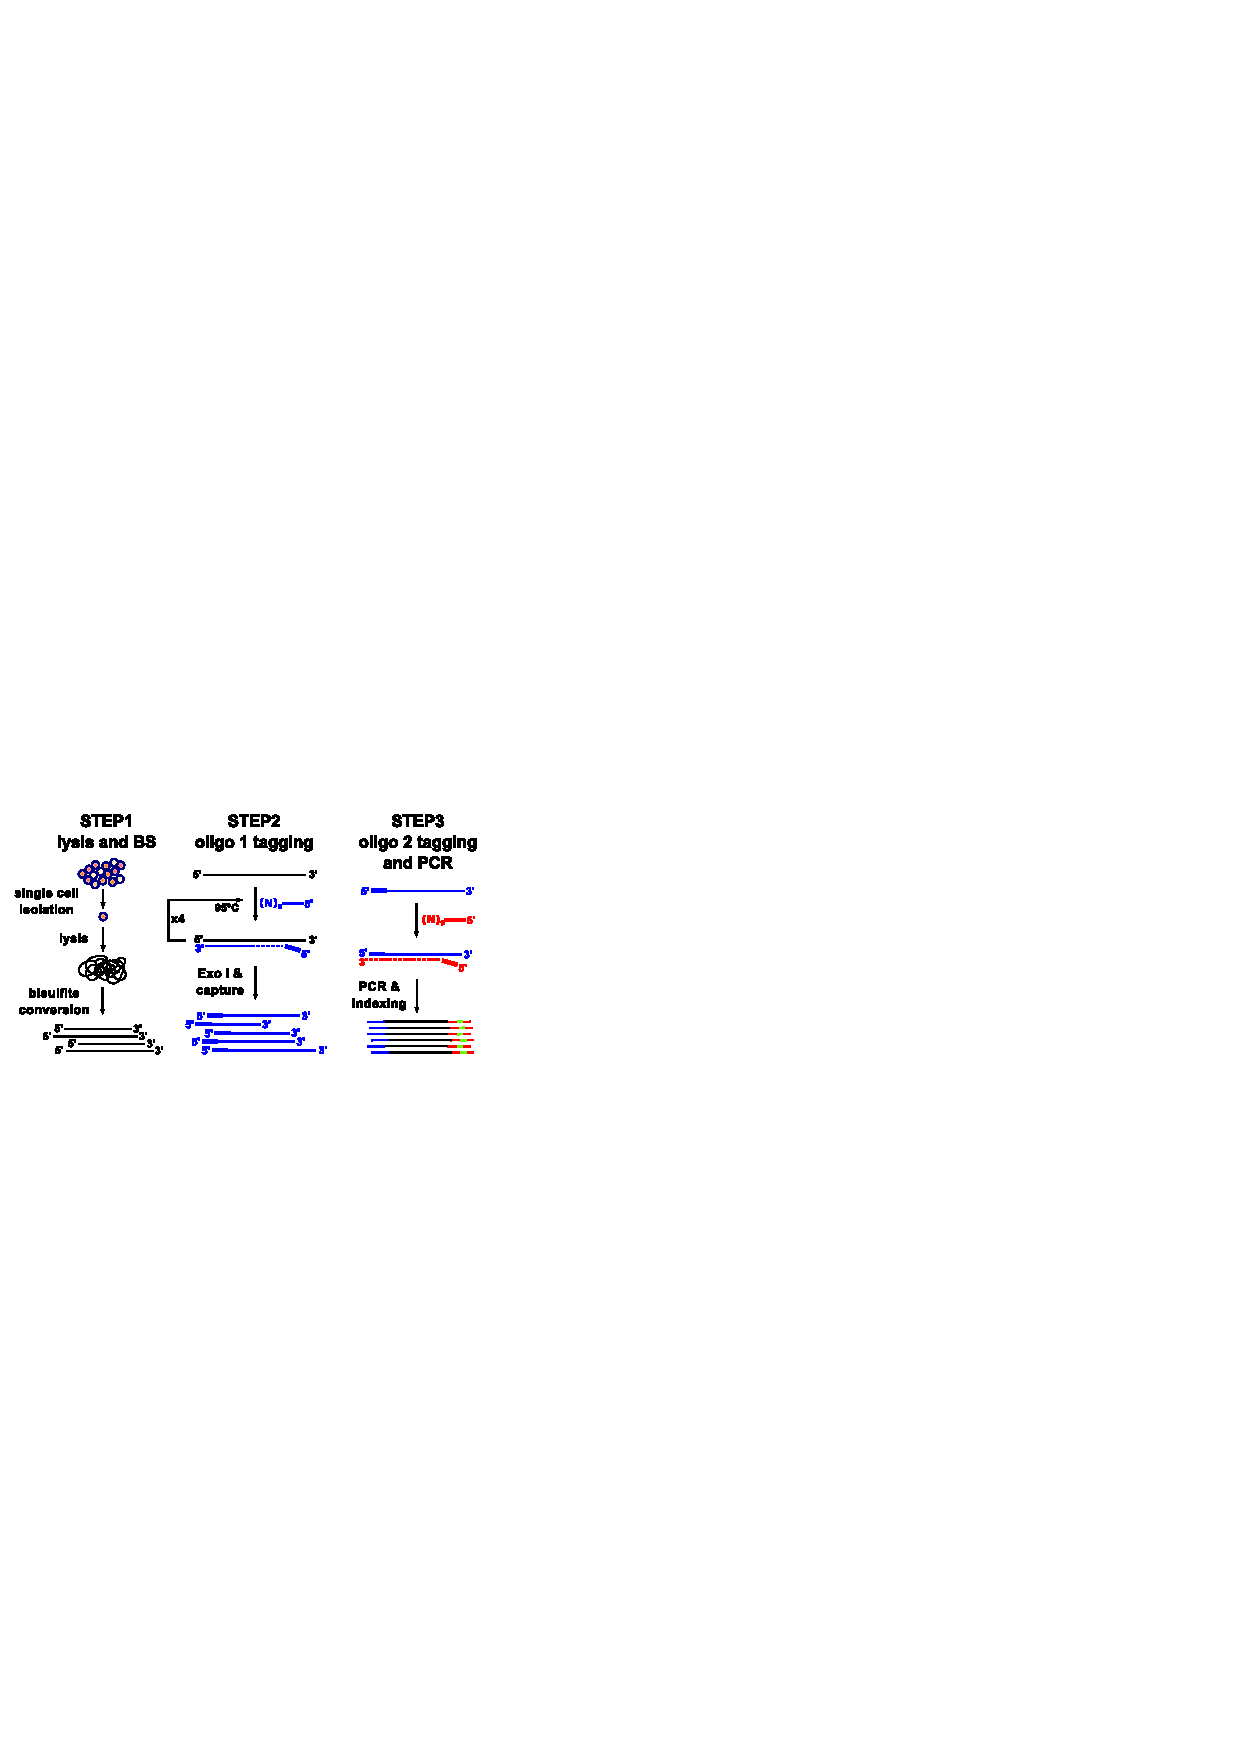
\includegraphics[width=0.75\textwidth]{proto}
\caption[scBS-seq profiling protocol.]{scBS-seq profiling protocol. scBS-seq library preparation consists of isolating and lysing single cells before bisulfite conversion (`BS'); performing five rounds of random priming and extension using oligo 1 (which carries the first sequencing adaptor) and purifying synthesized fragments; and performing a second random priming and extension step using oligo 2 (which carries the second sequencing adaptor) before amplifying the resulting fragments.}
\label{fig:bs_proto}
\end{figure}

We assessed scBS-seq on ovulated metaphase II oocytes (MIIs) and mouse ESCs cultured either in 2i medium or serum conditions. MIIs are a suited model for technical assessment as they: (i) can be individually hand- picked to ensure that only one cell is processed; (ii) represent a highly homogeneous population, which allows discrimination between technical and biological variability; and (iii) present a distinct DNA methylome comprising large-scale hypermethylated and hypomethylated domains~\citep{shirane_mouse_2013}. ESCs grown in serum conditions are characterized by a high heterogeneity in DNA methylation and gene expression and hence suited for the estimating of intercellular heterogenetiy~\citep{ficz_fgf_2013}. We used ESCs grown in serum (`serum ESCs') and ESCs grown in 2i medium (`2i ESCs') to determine whether scBS-seq can reveal DNA methylation heterogeneity in single cells.

We sequenced 12 MII, 12 2i ESC, 20 serum ESC, and 7 negative controls using scBS-seq, and their bulk cell counterparts using BS-seq. We obtained the methylation state of on average 3.7 million CpG dinucleotides (CpGs; range, 1.8 M–7.7 M) corresponding to 17.7\% of all CpGs (range, 8.5–36.2\%; \Cref{fig:bs_qc}~(a)). A higher CpG coverage can be obtained by deeper sequencing. To validate this, we sequenced two MII libraries close to saturation, which resulted in 1.5-fold and 1.9-fold more CpGs captured. Altogether, we obtained up to 10.1 M CpGs, corresponding to a CpG coverage of 48.4\%.

\begin{figure}[htbp!]
\centering
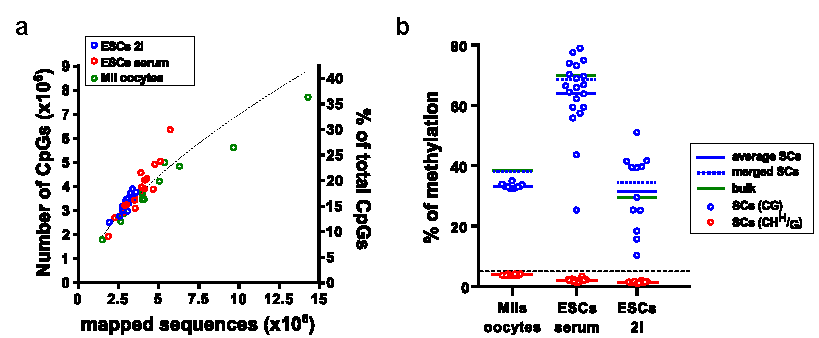
\includegraphics[width=0.8\textwidth]{qc}
\caption[scBS-seq mapping efficiency and mean methylation levels.]{scBS-seq mapping efficiency and mean methylation levels. (a) Number of CpGs obtained by scBS-seq as a function of mapped sequences. (b) Global mean DNA methylation levels in CpG (CG) and non-CpG (CHH/G) context for single cells (SCs), in silico–merged, and bulk samples. }
\label{fig:bs_qc}
\end{figure}

Next, we investigated the reproducibility and accuracy of scBS-seq. CpG sites in MIIs were overwhelmingly called methylated or unmethylated, which is consistent with a highly digitized output from single cells (\Cref{fig:bs_binary}). As expected, global methylation of MIIs was highly homogeneous ($33.1 \pm 0.8\%$) and 2i ESCs were hypomethylated compared to serum ESCs13. Yet both 2i ESCs and serum ESCs exhibited 5mC heterogeneity (serum, $63.9 \pm 12.4\%$; 2i medium, $31.3 \pm 12.6\%$; \Cref{fig:bs_qc}~(b)). We determined the average pairwise concordance between individual CpGs across single oocyte libraries, which was 87.6\% genome- wide (range, 85.3–88.9\%) and 95.7\% in unmethylated CGIs, a highly homogeneous genomic feature (\Cref{fig:bs_concord}~(a)). CpG concordance in ESCs was lower (serum, 72.7\%; 2i medium, 69.8\%), which reflected the heterogeneity of these cells (\Cref{fig:bs_concord}~(a)). At two kilo base pair (kbp) resolution, we observed high correlation between individual MIIs (Pearson's $r=0.92$), and between individual MIIs and bulk (Pearson's $r=0.95$) (\Cref{fig:bs_concord}~(b)). We could largely reproduce the entire bulk methylation profile of oocytes using only 12 single cells (\Cref{fig:bs_concord}~(b)). This capability is particularly beneficial for analyses of homogeneous cell populations and makes scBS-seq an important tool to investigate the 5mC landscape in very rare material.

\begin{figure}[htbp!]
\centering
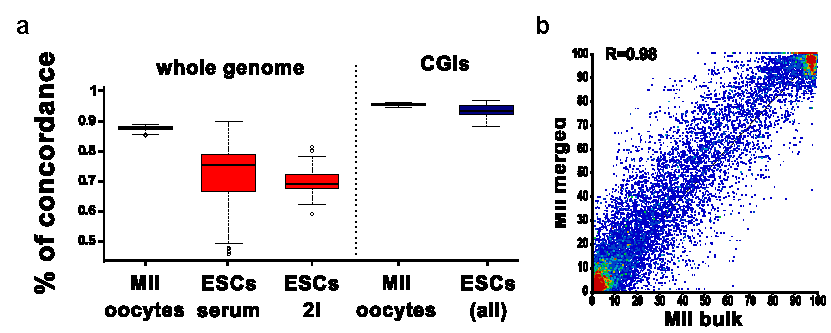
\includegraphics[width=1.0\textwidth]{concord}
\caption[CpG concordance and reproduction of bulk data.]{CpG concordance and reproduction of bulk data. (a) Pairwise analysis of CpG concordance genome-wide and in unmethylated CGIs. Boxplots represent the interquartile range, with the median; whiskers correspond to 1.5 times the interquartile range. (b) Pairwise correlation CpG methylation levels between MII-merged and MII-bulk data.}
\label{fig:bs_concord}
\end{figure}


\subsection{Method for estimating DNA methylation variability} \label{sec:bs_method}

The majority of CpG sites in single cells are either methylated or unmethylated. An exception is hemimethylation, where the cytosine is methylated on only one DNA strand. Consistent with this, scBS-seq called CpG sites overwhelmingly methylated or unmethylated (\Cref{fig:bs_binary}). Since hemimethylation is rare and currently hard to detect by scBS-seq owing to low CpG coverage, we did not consider hemimethylation in our analysis. Instead, we modelled the methylation state of CpG sites in single-cells as a Bernoulli variable, and represented methylation profiles as a binary matrix (\Cref{fig:bs_binary}). As a consequence of the limited CpG coverage of only ${\approx}10-30\%$, the methylation state of most CpG sites is unobserved, which renders downstream analyses challenging. We therefore developed a method that aggregates information from adjacent CpG sites and estimates mean methylation levels as well as cell-to-cell heterogeneity for windows instead of single CpG sites. Our method yields uncertainty estimates, which is critical in regions of low CpG coverage. Our method is further computational efficient, thereby applicable genome-wide on over 20 million CpG sites.

\begin{figure}[htbp!]
\centering
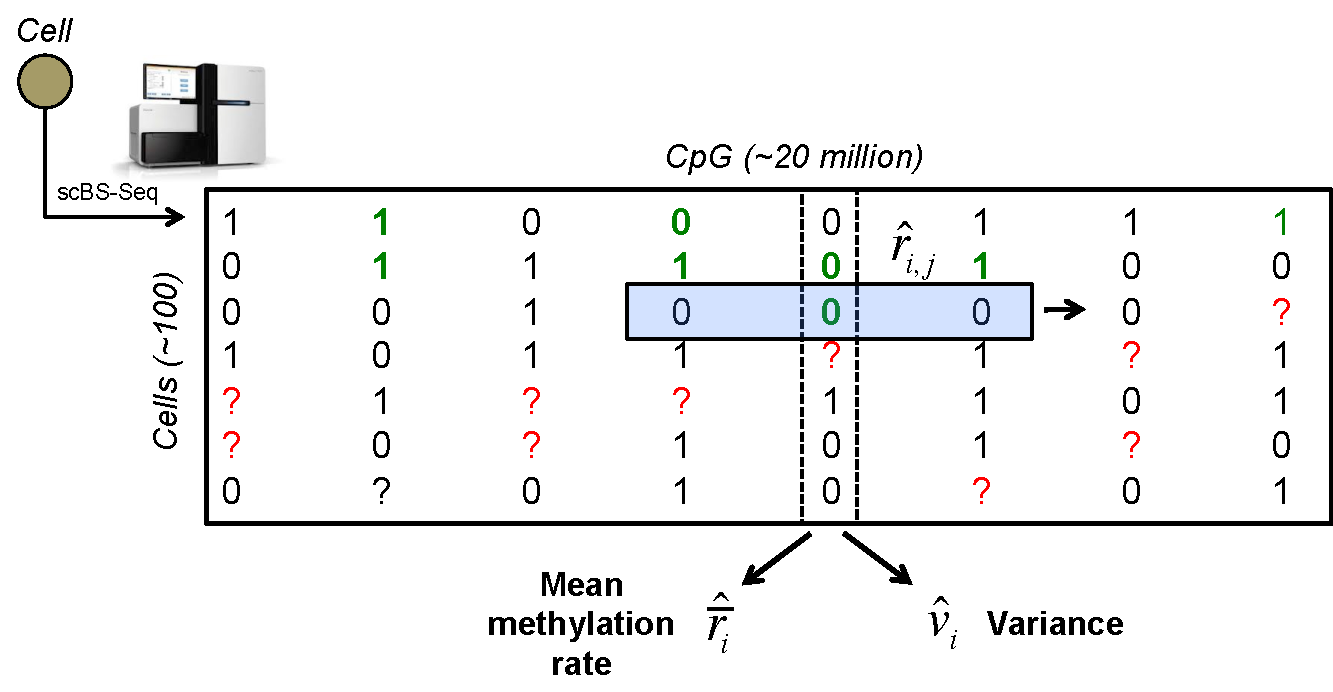
\includegraphics[width=0.9\textwidth]{method}
\caption[Representation of single-cell methylation data.]{Representation of single-cell methylation data. Binary matrix $M$ with rows corresponding to cells and columns to CpG sites. $M_{i,j}$ represent the methylation state of CpG site $i$ in cell $j$, which is one if the CpG site is methylated and zero otherwise. Question marks denote sites with unobserved methylation state. A sliding window (blue) is used to first estimate the methylation rate $\hat{r}_{i,j}$ (green) for each cell and window, and the mean methylation rate $\hat{\bar{r}}_i$ and variance $\hat{v}_i$ across cells afterwards.}
\label{fig:bs_method}
\end{figure}


\newcommand{\Xfw}{c^+}
\newcommand{\Xrv}{c^-}
\newcommand{\Xfws}{s^+_{i,j}}
\newcommand{\Xrvs}{s^-_{i,j}}
\newcommand{\XBin}{\operatorname{Bin}}
\newcommand{\Xse}{\operatorname{SE}}
\newcommand{\Xrij}{\hat{r}_{i,j}}
\newcommand{\Xri}{\hat{r}_i}
\newcommand{\Xwij}{w_{i,j}}
\newcommand{\Xrmi}{\hat{\overline{r}}_i}
\newcommand{\Xrvi}{\hat{v}_i}
\newcommand{\Xrvli}{\hat{v}^l_i}
\newcommand{\Xrvui}{\hat{v}^u_i}
\newcommand{\Xwjji}{w^{j,j^\prime}_i}


\subsubsection{Estimating cell-specific methylation rates}

To increase the coverage across cells, we employed a sliding window approach, which is conceptually similar to approaches that have been used for bulk BS-Seq~\citep{bock_dna_2012,li_dna_2010}. With window size $w=3000$~bp and step size 600~bp, we computed for each cell $j$ the sum of methylated $c^+_{i,j}$ and unmethylated $c^-_{i,j}$ read counts in window $i$:
\begin{align}
  \Xfws = \sum_{k=-w/2}^{+w/2} \Xfw_{i+k, j} \qquad
  \Xrvs = \sum_{k=-w/2}^{+w/2} \Xrv_{i+k, j}
\end{align}
To estimate methylation rates, we modelled the sum $S^+_{i,j}$ of methylated read counts as a Binomial random variable with methylation rate $r_{i,j}$:
\begin{align}
  S^+_{i,j}\sim \XBin(\Xfws+\Xrvs, r_{i,j})
\end{align}
Assuming $r_{i,j}\sim \operatorname{Beta}(1,1)$, leads to the maximum a posteriori estimator $\hat{r}_{i,j}$ of the methylation rate in cell $j$ and window $i$:
\begin{align}
  \Xrij = \frac{\Xfws+1}{\Xfws+\Xrvs+2}
\end{align}
To account for the limited CpG coverage of scBS-seq (\Cref{sec:bs_proto}), we quantified prediction uncertainty by approximating the standard error of the rate estimator using the Wald method~\citep{stein_sequential_1947}:
\begin{align}
  \Xse[\Xrij]^2 = \frac{\Xrij(1-\Xrij)}{\Xfws+\Xrvs}
\end{align}


\subsubsection{Estimating cell-to-cell variability}

We used the estimated cell-specific methylation rates $\Xrij$ to estimate the mean methylation rate and variance across all cells. We modelled the mean methylation rate $r_i$ in window~$i$ as a Gaussian random variable with mean $\overline{r}_i$ and variance $v_i$:
\begin{align}
  r_i \sim N(\overline{r}_i, v_i)
\end{align}
To account for differences in the standard errors $\Xse[\Xrij]$, we weighted cell $j$ and position $i$ by $\Xwij=\Xse[\Xrij]^{-2}$, and used the weighted maximum likelihood estimator
\begin{align}
  \Xrmi = \frac{1}{\sum_j \Xwij} \sum_j \Xwij\Xrij
\end{align}
to estimate $\overline{r}_i$. Its standard error is given by
\begin{align}
  \Xse[\Xrmi]^2 = \frac{1}{\sum_j \Xwij}.
\end{align}
The maximum likelihood estimator of the variance $v_i$ is
\begin{align} \label{eq:bs_var}
  \Xrvi = \frac{\sum_j \Xwij}{\left(\sum_j \Xwij\right)^2 - \sum_j \Xwij^2} \sum_j \Xwij \left(\Xrij - \Xrmi\right)^2,
\end{align}
which is the unbiased weighted cell-to-cell variance. The chi-squared confidence interval of the variance estimator with significance level $\alpha$ is
\begin{align}
  [\Xrvli, \Xrvui] = [\frac{n_i \Xrvi}{\chi^2_{1-\frac{\alpha}{2}, n_i}},
  \frac{n_i \Xrvi}{\chi^2_{\frac{\alpha}{2}, n_i}}].
\end{align}
Here, $\chi^2_{p, n_i}$ is the $p$-quantile of the chi-squared distribution with $n_i$ degrees for freedom, where $n_i$ is the sum of cell weights:
\begin{align}
  n_i^2 = \frac{\sum_j \Xwij}{\left(\sum_j \Xwij\right)^2 - \sum_j \Xwij^2}
\end{align}
To determine highly variable methylated sites, we ranked these by the lower bound $\Xrvli$ of the chi-squared confidence interval and defined the top k sites as the most variable sites. This approach is selecting sites with large estimates of cell-to-cell variance while penalizing for uncertainty of these estimates due to low CpG coverage.

\subsubsection{Cluster analysis}

To cluster cells and sites, we considered a complete linkage clustering, and employed the weighted Euclidean norm as distance measure for comparing cell $j$ with cell $j^\prime$:
\begin{align} \label{eq:bs_clust}
  d(j, j^\prime) = \sqrt{\sum_{i=1}^d \Xwjji \left(\hat{r}_{i,j} - \hat{r}_{i, j^\prime}\right)^2}
\end{align}
We defined the weight $\Xwjji$ at position $i$ as
\begin{align}
  \Xwjji \propto \sqrt{w_{i,j}w_{i,j^\prime}},
\end{align}
and normalized weights to sum up to the total number of positions $d$. This distance measure places most emphasis on positions that are covered by both cells.


\subsection{Methylation variability in different genomic contexts} \label{sec:bs_results}

\begin{figure}[htbp!]
\centering
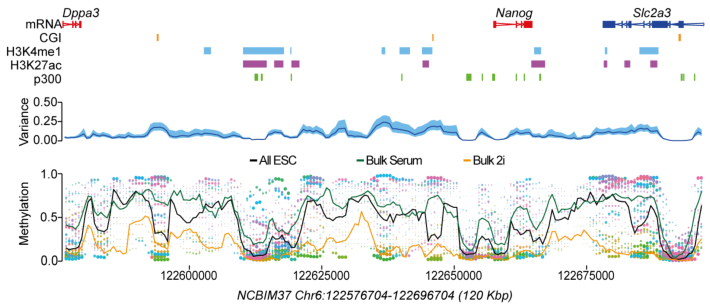
\includegraphics[width=1.0\textwidth]{zoom}
\caption[Estimated methylation rates for Nanog locus.]{Estimated DNA methylation rates using a sliding window in an example region containing the Nanog locus with some annotated features. Each single ESC is represented by a different color (bottom), and dot size is the inverse of estimation error. Mean methylation rate estimates across cells (black line, bottom) and cell-to-cell variance (blue line, middle; 95\% confidence interval in light blue) are shown. Methylation rates for `bulk serum' (green line) and `bulk 2i' (orange line) are superimposed (bottom).}
\label{fig:bs_zoom}
\end{figure}

We applied our method to estimate methylation rates in each ESC genome as well as the mean methylation rate and variance across all ESCs (\Cref{fig:bs_zoom}). By using our method for weighted clustering (\Cref{eq:bs_clust}), we identified two distinct clusters that represented the majority of 2i ESCs and serum ESCs (\Cref{fig:bs_clust}~(a)). Two outlier cells from the serum condition clustered with 2i ESCs, which implies that serum cultures contain `2i-like' ESCs and demonstrates the ability of scBS-seq to identify rare cell types in populations. To examine 5mC heterogeneity in ESCs in greater detail, we ranked sites by the estimated cell-to-cell variance (\Cref{eq:bs_var}) and repeated the cluster analysis for the 300 most variable sites (\Cref{fig:bs_top300}). The structure of the resulting clusters was broadly similar to what was observed based on genome-wide analysis, and all 300 variable sites followed the global trend of being more highly methylated in serum than 2i ESCs with high similarity between sites (\Cref{fig:bs_qc}~(b); \Cref{fig:bs_top300}). This observation is consistent with the genome-wide hypomethylation observed in ESCs grown in 2i medium~\citep{ficz_fgf_2013} and indicates that a major determinant of ESC heterogeneity is global methylation.

\begin{figure}[htbp!]
\centering
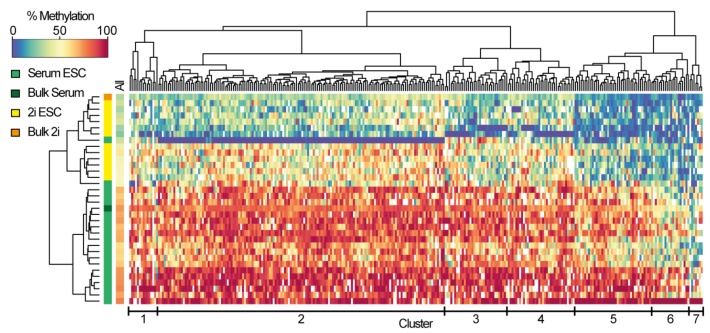
\includegraphics[width=1.0\textwidth]{top300}
\caption[Heatmap of 300 most variable sites.]{Heatmap for methylation rates of the 300 most variable sites among single-cell ESC samples. Cluster dendrograms for samples (left) and sites (top) are shown. The genome-wide average methylation rate is displayed in the left track (`all'). The main clusters of variable sites are indicated at the bottom.}
\label{fig:bs_top300}
\end{figure}

Our method also identified sites whose methylation varied more than the genome average, including sites with marked heterogeneity even among cells from the same growth condition (e.g. clusters 5 and 6 in serum ESCs; \Cref{fig:bs_top300}). Regions containing H3K4me1 and H3K27ac, marks associated with active enhancers, had the greatest variance in 5mC, whereas CGIs and intracisternal A-particle repeats had lower variance than the genome average (\Cref{fig:bs_clust}~(b)). These findings are consistent with observations that distal regulatory elements are differentially methylated between tissues and throughout development~\citep{stadler_dna-binding_2011,ziller_charting_2013,hon_epigenetic_2013}

\begin{figure}[htbp!]
\centering
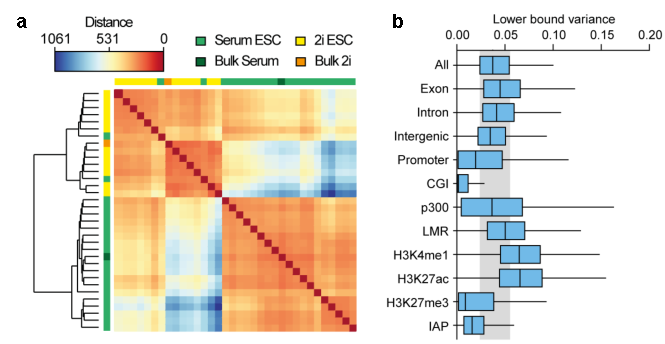
\includegraphics[width=1.0\textwidth]{clust}
\caption[Genome-wide clustering and estimated variance in genomic contexts.]{Genome-wide clustering and estimated variance in genomic contexts. (a) Genome-wide cluster dendrogram and distance matrix for all ESCs and bulk samples based on estimated methylation rates. Distance refers to the weighted Euclidean norm between estimated rates. (b) Variance of sites located in different genomic contexts. Boxes represent interquartile range with the median; whiskers correspond to 1.5 times the interquartile range. The shaded gray region indicates the interquartile range for all genome-wide sites.}
\label{fig:bs_clust}
\end{figure}

\section{Estimating associations between DNA methylation and gene expression} \label{sec:mt}

\ifpdf
    \graphicspath{{Chapter3/mt/Figs/Raster/}{Chapter3/mt/Figs/PDF/}{Chapter3/mt/Figs/}}
\else
    \graphicspath{{Chapter3/mt/Figs/Vector/}{Chapter3/mt/Figs/}}
\fi

We have shown that scBS-seq enables the exploration of intercellular heterogeneity in DNA methylation genome-wide. To further study the relationship between heterogeneity in DNA methylation and gene expression, we developed scM\&T-seq, a protocol for parallel profiling of DNA methylation and gene expression in single cells. In combination with scM\&T-seq, we developed methods for estimating associations between DNA methylation and gene expression in single cells, which will be described in the following.

\subsection{Parallel single-cell DNA methylation and gene expression profiling}

\citet{macaulay_g&t-seq:_2015} have recently developed G\&T-seq, a method for parallel genome and transcriptome sequencing within single cells. Importantly, G\&T-seq utilizes physical separation of RNA and DNA allowing bisulfite conversion of DNA without affecting the transcriptome. We now apply scBS-seq to genomic DNA purified according to the G\&T-seq protocol. Our scM\&T-seq protocol consists of isolating single cells, followed by physical separating DNA and RNA using the G\&T protocol (\Cref{fig:mt_proto}). DNA is bisfulfite treated and sequenced using scBS-seq to quantify DNA methylation of individual cells, and RNA is sequenced using scRNA-seq~\citep{jaitin_massively_2014} to quantify gene expression.

\begin{figure}[htbp!]
  \begin{minipage}[c]{0.65\textwidth}
    \centering
    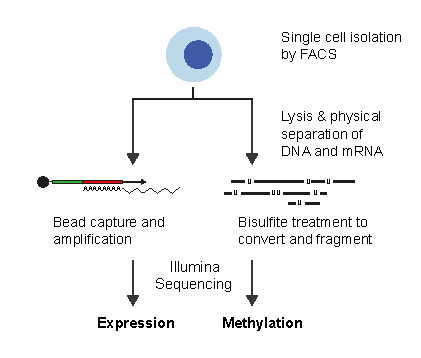
\includegraphics[width=1.0\textwidth]{proto}
  \end{minipage}
  \begin{minipage}[c]{0.32\textwidth}
    \caption[Schematic overview of the scM\&T-seq protocol.]{Schematic overview of the scM\&T-seq protocol. Single-cells are isolated by FACS sorting and extracted DNA separated from RNA using G\&T-seq. DNA is treated with bisulfite and sequenced using scBS-seq to quantify DNA methylation; RNA is amplified and sequences to quantify gene expression.}
    \label{fig:mt_proto}
  \end{minipage}
\end{figure}

We evaluated scM\&T-seq on mouse ESCs. In the presence of serum, these cells are characterized by high transcriptional and epigenetic heterogeneity. To investigate the link between epigenetic and transcriptional heterogeneity in ESCs, we performed scM\&T-seq on 76 individual serum ESCs and 16 ESCs grown in `2i' media, which induces genome-wide DNA hypomethylation.

To assess the quality of the scBS-seq data, we compared the resulting single-cell methylomes with the 20 serum and 12 2i ESCs that we profiled with stand-alone scBS-seq (\Cref{sec:bs_proto}). The genome-wide CpG coverage at matched sequencing depth was consistent across scM\&T-seq and scBS-seq (\Cref{fig:mt_qc}~(a)) and we found that scM\&T-seq covered a large proportion of sites in different genomic contexts with sufficient frequency to enable the analysis of epigenome heterogeneity across cells. As additional validation, we assessed the discrimination of serum and 2i ESCs by both stand-alone scBS-seq and scM\&T-seq, finding a similar degree of separation that was consistent with bulk datasets published previously~\citep{ficz_fgf_2013} (\Cref{fig:mt_qc}~(b)), with similar conclusions when using a joint hierarchical clustering across all cells (\Cref{fig:mt_clust}). Notably, the difference between protocols and biological batches had a substantially smaller effect (PC2, 3\% variance) than cell type differences (PC1, 48\% variance), and by combining data across cells, we found that both protocols yield genome-wide methylation profiles that accurately recapitulate bulk methylation profiles in the same cell type (\Cref{fig:mt_bulk}). Finally, we compared estimates of methylation heterogeneity in different genomic contexts, again finding good agreement between protocols (\Cref{fig:mt_var}). Taken together, these analyses provide confidence that the parallel scM\&T-seq method yields results that are in agreement with data from stand-alone scBS-seq.

\citet{macaulay_g&t-seq:_2015} has previously shown that the scRNA-seq data generated by the G\&T-seq method is of similar quality to that generated using the scRNA-seq protocol. We obtained an average of 2.7 million scRNA-seq reads per cell, and we excluded cells with fewer than 2 million mapped reads. In ESCs that met scRNA-seq quality-control criteria, we detected transcripts from between 4000 and 8000 genes exceeding one transcript per million, consistent with previous measurements made using the method (\Cref{fig:mt_qc_rna}).

\begin{figure}[htbp!]
\centering
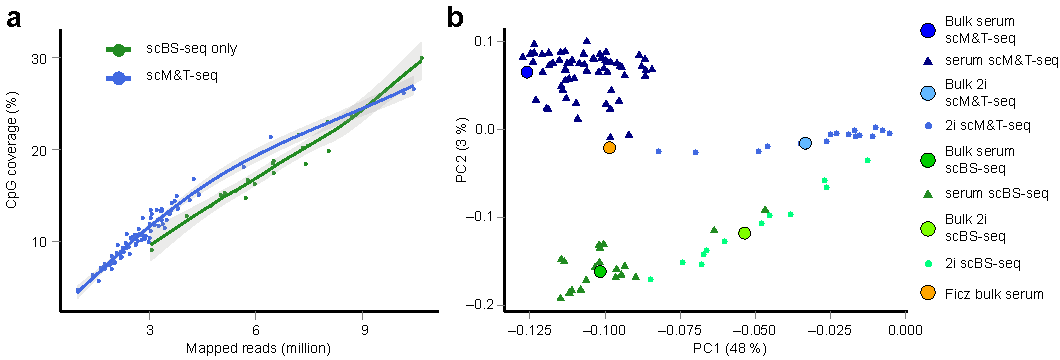
\includegraphics[width=1.0\textwidth]{qc}
\caption[Quality controls of scM\&T-seq protocol.]{Schematic overview of the scM\&T-seq protocol. (a) CpG coverage of single cells as a function of the number of mapped sequencing reads. Green: stand-alone scBS-seq, Blue: scM\&T-seq. (b) Joint principal component analysis of the methylomes (gene body methylation) of 61 serum ESCs (dark blue) and 16 2i ESCs (light blue) obtained using scM\&T-seq, as well as 20 serum ESCs (green) and 12 2i ESCs (yellow) sequenced using stand-alone scBS-seq. The solid circles correspond to synthetic bulk datasets form the same cells. For comparison, we also included a bulk serum ESC DNA methylation dataset~\citep{ficz_fgf_2013} (orange). Cell type explained a substantially larger proportion of variance (PC1, 48\%) than protocol (PC2, 3\%).}
\label{fig:mt_qc}
\end{figure}

For subsequent analyses, we focused on serum ESCs only since transcription and DNA methylation are uncoupled in 2i ESCs~\citep{ficz_fgf_2013,habibi_whole-genome_2013}. A comparison of the principal components derived from gene body methylation and gene expression revealed associations between some factors of variations of both data modalities (\Cref{fig:mt_cca}; \Cref{fig:mt_cca_cor}). However, a hierarchical clustering analysis of gene body methylation and gene expression for the 300 most variable genes revealed distinct clustering of cells when using either source of information (\Cref{fig:mt_heat}). This suggests that global methylome and transcriptome profiles yield complementary but distinct aspects of cell state. This is also consistent with previous observations that the transcriptome and methylome are partially uncoupled in serum ESCs~\citep{ficz_fgf_2013}.

\begin{figure}[htbp!]
\centering
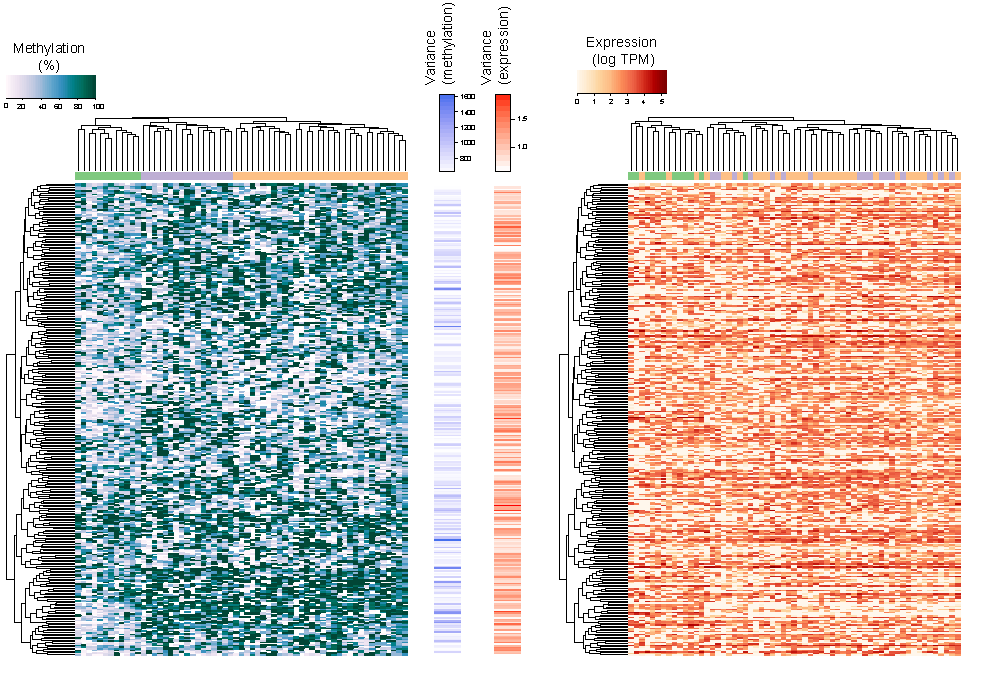
\includegraphics[width=1.0\textwidth]{heat}
\caption[Clustering analysis of transcriptome and methylome data.]{Clustering analysis of transcriptome and methylome data from 61 serum ESCs, considering gene body methylation (left) and gene expression (right) for the 300 most heterogeneous genes (based on gene body methylation). The order of genes was taken from an individual clustering analysis based on gene body methylation whereas cells were clustered separately either using DNA methylation or expression data, and coloured by methylation cluster. The bar plots in the center show the heterogeneity in DNA methylation (left) and gene expression (right).}
\label{fig:mt_heat}
\end{figure}


\subsection{Methods for estimating associations between DNA methylation and gene expression} \label{sec:mt_method}

\newcommand{\Xcov}{\operatorname{cov}}
\newcommand{\Xcor}{\operatorname{cor}}

\begin{figure}[htbp!]
\centering
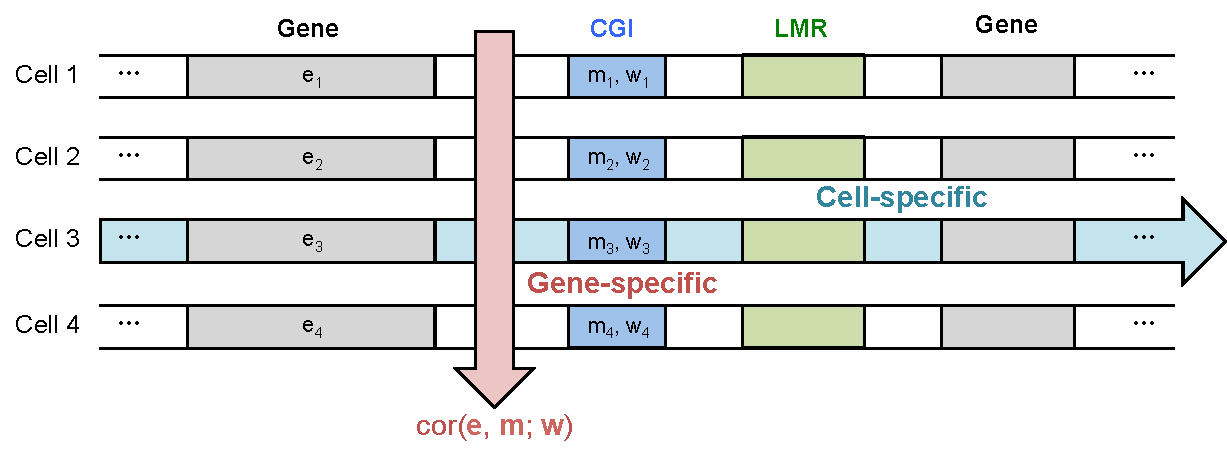
\includegraphics[width=1.0\textwidth]{method}
\caption[Schematic representation cell-specific and gene-specific correlation analysis between methylome and transcriptome.]{Schematic representation cell-specific and gene-specific correlation analysis between methylome and transcriptome. Cell-specific analysis is performed for a single cell or a bulk population of cells across multiple genes. Gene-specific analysis is performed for a single gene across multiple cells. The vector $e$ represents the expression rates of the considered gene for all cells, $m$ the mean methylation rates in the corresponding genomic context, and $w$ the number of covered CpG sites within that context. Associations were estimated by the weighted Pearson correlation $\Xcor(e, m; w)$ to account for differences in CpG coverage between cells.}
\label{fig:mt_method}
\end{figure}

Previous studies on data from bulk sequencing protocols estimated correlations between methylome and transcriptome in a bulk population of cells across multiple genes (\Cref{fig:mt_method}). In contrast, scM\&T-seq separates individual cells and hence enables estimating associations for a particular gene across multiple cells. Let $e$ be a vector with expression rates of cells for a particular gene, $m$ be methylation rates of the associated region, and $w$ be weights corresponding to the number of covered CpGs sites within the region. Then we estimated associations using weighted Pearson correlation $\operatorname{cor}(e,m;w)$ between gene-expression $e$ and methylation $m$:
\begin{align} \label{eq:mt_wcor}
  \Xcor(e,m;w)=\frac{\Xcov(e,m;w)}{\sqrt{\Xcov(e,e;w)\Xcov(m,m;w)}}
\end{align}
Here, $\Xcov(x,y;w)$ is the weighted covariance
\begin{align}
  \Xcov(x,y;w)=\sum_i \frac{w_i (x_i-m(x;w))(y_i-m(y;w))}{\sum_i w_i },
\end{align}
and $m(x;w)$ the weighted arithmetic mean:
\begin{align}
  m(x;w)=\frac{\sum_i x_i w_i}{\sum_i w_i}
\end{align}
By computing weighted correlations, we accounted for differences in CpG coverage between cells. We considered all possible relationships between genes and methylated regions within 10~kbp of the gene (upstream and downstream of gene start or stop). We performed two-sided Student's t-tests to test for non-zero correlations, and adjusted p-values for multiple testing for each context using the Benjamini-Hochberg procedure.

We considered gene expression levels on a logarithmic scale using log10 normalized TPM counts. We estimated binary single-base pair CpG methylation states by the ratio of methylated read counts to total read counts. We further estimated the methylation rate in different genomic contexts, such as gene body, promoter, or enhancer annotations, as the mean CpG methylation rate within the region defined by the context.

We discarded genes with low expression levels or low expression and methylation variability between cells, following the rational of independent filtering~\citep{bourgon_independent_2010}. First, a minimum expression level (at least 10 TPM counts) in at least 10\% of all cells was required. From these, the 7500 most variable genes were considered for analysis. Second, methylated regions were required to be covered by at least one read in at least 50\% of all cells.


\subsection{Associations between DNA methylation and gene expression in different genomic contexts} \label{sec:mt_results}

Using weighted Pearson correlation (\Cref{eq:mt_wcor}), we tested for associations between expression of individual genes and DNA methylation variation at several genomic contexts. We identified a total of 1493 associations ($\FDR<0.1$; \Cref{fig:mt_gene_volcano}), which were robust when using a bootstrapping approach to subsample the set of cells. We found both positive and negative associations, highlighting the complexity of interactions between the methylome and transcriptome~\citep{dey_integrated_2015}. While methylation of non-CGI promoters is known to be associated with transcriptional repression, the role of enhancer methylation is less clear. Accordingly, negative correlations between DNA methylation and gene expression were predominant for non-CGI promoters, whereas positive and negative associations were more balanced in distal regulatory elements including LMRs (\Cref{fig:mt_gene_volcano}; \Cref{fig:mt_gene_r}; \Cref{fig:mt_gene_volcano_all}). Interestingly, associated genes were enriched for known pluripotency and differentiation genes~\citep{kolodziejczyk_single_2015} ($\FDR<0.01$, Fisher's exact test). Our results provide the first evidence that heterogeneous methylation of distal regulatory elements, e.g. LMRs, accompanies heterogeneous expression of key pluripotency factors in stem cell populations~\citep{lee_reprogramming_2014}.

\begin{figure}[htbp!]
\centering
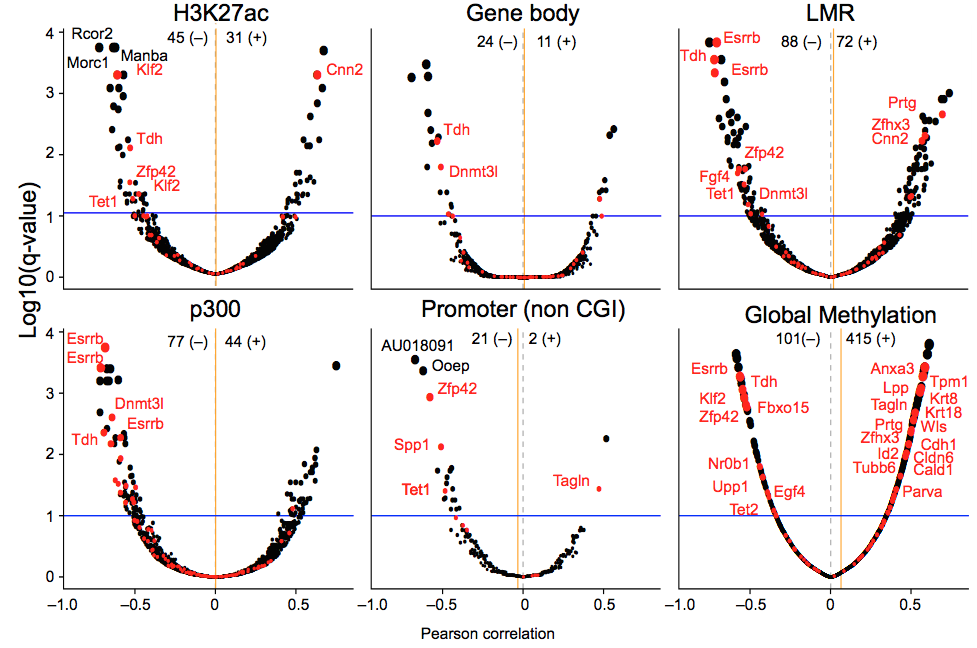
\includegraphics[width=0.8\textwidth]{gene_volcano}
\caption[Volcano plots of correlation coefficients.]{Volcano plots of correlation coefficients (Pearson's $r^2$) from association tests between gene expression heterogeneity of individual genes and DNA methylation heterogeneity in alternative genomic contexts. Shown is the correlation coefficient for every gene (x-axis) versus the adjusted p-value (using Benjamini-Hochberg correction; y-axis). The size of dots corresponds to the adjusted p-value. A set of 86 known pluripotency and differentiation genes are highlighted in red. The blue horizontal line corresponds to the $\FDR=0.1$ significance threshold. The total number of significant positive (+) and negative (–) correlations ($\FDR<0.1$) for each annotation is shown in the header of each panel. The orange vertical bar corresponds to the average correlation coefficient across all genes for a given context.}
\label{fig:mt_gene_volcano}
\end{figure}

As an example, \cref{fig:mt_zoom} shows the association map of Esrrb--a known key regulator gene in pluripotency networks~\citep{papp_pluripotency_2012}. Expression of Esrrb negatively correlated with the methylation of several LMR and p300 sites overlapping `super enhancers' in the genomic neighbourhood~\citep{whyte_master_2013}, providing evidence for the regulatory importance of Esrrb. We also found 516 genes whose expression correlated with the overall methylation level ($\FDR<0.1$), indicating substantial links between transcriptional heterogeneity and global methylation levels (\Cref{fig:mt_gene_volcano}).

\begin{figure}[htbp!]
\centering
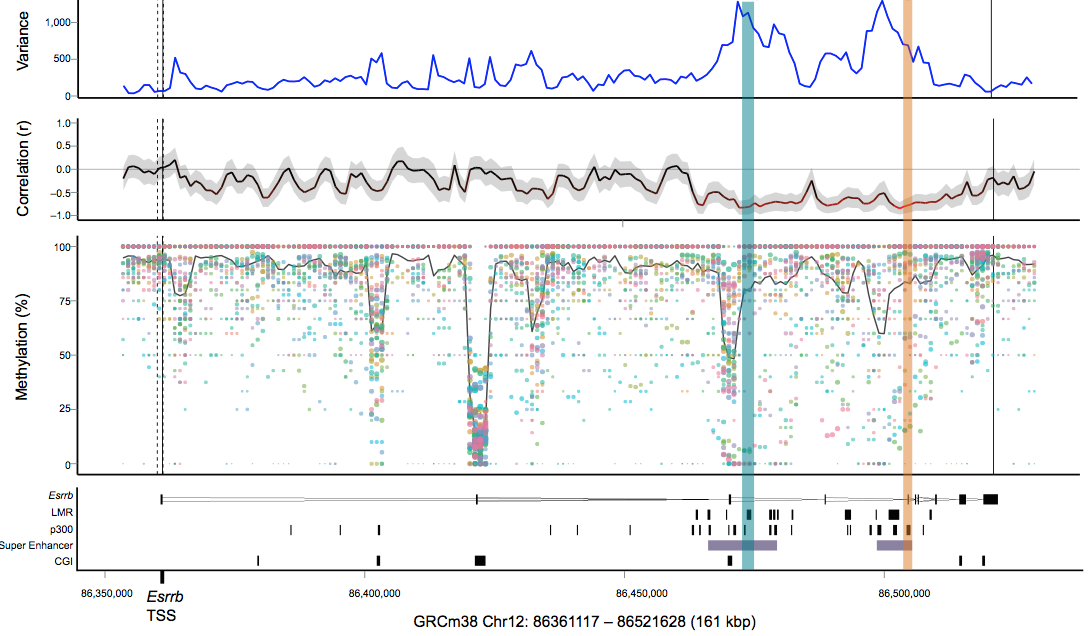
\includegraphics[width=1.0\textwidth]{zoom}
\caption[Representative zoom-in view for the gene Esrrb.]{Representative zoom-in view for the gene Esrrb. From bottom to top, shown is: the annotation of the Esrrb locus with LMR, p300, super enhancer and CGI sites indicated; the estimated methylation rate of $3~kbp$ windows for each cell with the size of dots representing the CpG coverage and the solid line indicating the weighted mean methylation rate across all cells; the correlation between the methylation rate and Esrrb expression for each region coloured by the strength of the correlation and with the shaded area corresponding to the 95\% confidence interval of the correlation coefficient; and the estimated weighted DNA methylation variance between cells. The vertical bars denote the location of a p300 (yellow) and LMR (blue) region, in which DNA methylation is significantly associated with gene expression.}
\label{fig:mt_zoom}
\end{figure}

In addition to between-cell analyses, scM\&T-seq can be used to correlate the methylome and transcriptome between genes in individual cells (\Cref{fig:mt_method}; \Cref{fig:mt_cell}), analogously to studies in cell populations. We found that correlation between methylation and gene expression varied substantially between cells but was consistent in direction with matched RNA-seq and BS-seq data from a population of cells~\citep{ficz_fgf_2013}. Again, this attests to scM\&T-seq being sufficiently accurate to reliably study epigenome-transcriptome linkages. Our results also point to the possibility of heterogeneity between cells in the degree of coupling between the methylome and the transcriptome. Although we have ruled out obvious confounding factors, such as average methylation rate and sequence coverage (\Cref{fig:mt_cell_r_mean}; \Cref{fig:mt_cell_r_cov}), more data will be required to understand possible technical components in these linkages.

\begin{figure}[htbp!]
\centering
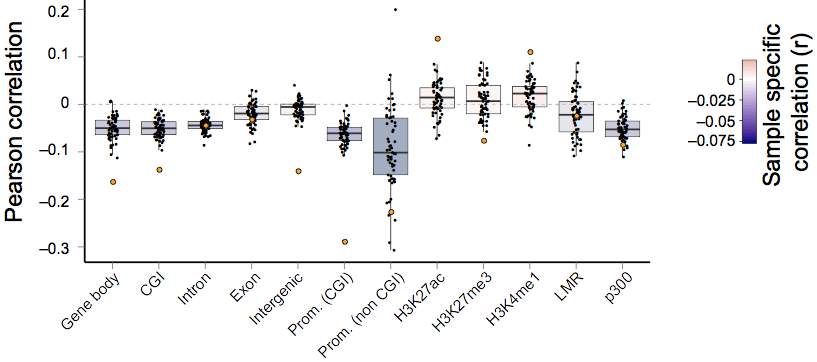
\includegraphics[width=1.0\textwidth]{cell}
\caption[Cell-specific correlation analysis]{Cell-specific association analysis, estimating correlations between DNA methylation in different genomic contexts and gene expression in individual cells. For each annotation, shown are box plots of methylation-expression correlations for all variable genes in single cells, with the correlation obtained from matched RNA-seq and BS-seq of a bulk cell population superimposed (orange circles).}
\label{fig:mt_cell}
\end{figure}



\section{Discussion}

We have first presented scBS-seq for profiling DNA methylation in single cells and a statistical model for quantifying methylation heterogeneity in cell populations at a genome-wide scale. We demonstrated that our approach detects rare cell types in populations and identifies genomic regions with high methylation heterogeneity that are functionally important during cell differentiation.

We further extended our protocol for parallel profiling of the methylome and transcriptome from the same single cell, allowing the relationship between DNA methylation and expression to be explored. We confirmed a negative association between non-CGI promoter methylation and transcription in single cells and identified both positive and negative associations at distal regulatory regions. We found the expression levels of many pluripotency factors, e.g. Esrrb, to be negatively associated with DNA methylation. Furthermore, we demonstrated that the strength of the connection between methylome and transcriptome can vary from cell to cell.

We used principal component analysis to investigate the factors of variations of DNA methylation and gene expression. To better understand the relation between these factors and to distinguish between factors that drive variations either in DNA methylation or gene expression, future studies may consider advanced statistical methods such as canonical correlation analysis or collective matrix factorization.

In our study, we only considered correlations between genes and genomic regions with a maximum genomic distance of 10~kbp. An important area of future research is to investigate trans-associations between DNA methylation and gene expression. For this, chromatin contact information from Hi-C experiments can be considered to identify distal genomic regions that are in close spatial proximity with a certain gene.

We estimated mean methylation rates in genomic context by averaging and used weighted Pearson correlation to account for incomplete CpG coverage. More sophisticated methods to estimate the mean methylation rate in genomic context from low-coverage data may reveal stronger associations between DNA methylation and gene expression. These include methods for imputing CpG methylation in single cells, which will be discussed in the following chapter.

%!TEX root = ../thesis.tex
%*******************************************************************************
%****************************** Third Chapter **********************************
%*******************************************************************************
\chapter{Deep neural networks for predicting DNA methylation} \label{sec:dcpg}

% **************************** Define Graphics Path **************************
\ifpdf
    \graphicspath{{Chapter4/Figs/Raster/}{Chapter4/Figs/PDF/}{Chapter4/Figs/}}
\else
    \graphicspath{{Chapter4/Figs/Vector/}{Chapter4/Figs/}}
\fi

Protocols for profiling DNA methylation in single cells are powerful for studying intercellular differences. However, they are limited by incomplete CpG coverage, which renders downstream analyses challenging. We therefore developed a deep neural network, \emph{DeepCpG}, for imputing incomplete DNA methylation profiles in single cells. In this chapter, we will describe the architecture of DeepCpG and show that it yields considerably more accurate predictions than existing methods across alternative cell types and sequencing protocols. In \cref{sec:dcpg_ana}, we will then present methods for analysing DNA methylation in single cells using DeepCpG. The presented work is based on \citet{angermueller_accurate_2017}.


\section{Motivation}

Single-cell DNA profiling technologies enabled the fine-grained study of DNA methylation in single cells. However, neither genome-wide (scBS-seq; \Cref{sec:bs}) nor reduced representation (scRRBS-seq; \Cref{sec:intro_proto}) protocols cover all CpG sites per cell. scBS-seq is limited by its efficiency to capture DNA and read-mapping biases, resulting in a CpG coverage of 10-30\% per cell. scRRBS-seq is limited to genomic regions of high CpG density by design, resulting in a CpG coverage of 1-10\% per cell. Unlike scBS-seq, scRRBS-seq is systematically biased towards CpG dense regions, making it impossible to obtain genome-wide CpG coverage by pooling cells.

The low CpG coverage renders several downstream analyses challenging, for example quantifying DNA methylation variability between cells (\Cref{sec:bs_method}), clustering cells (\Cref{sec:bs_method}), or correlating DNA methylation with gene expression. Whereas data of low CpG coverage can already be sufficient to reliably estimate average DNA methylation levels in large or CpG dense regions such as gene bodies or CGIs, analysing small or CpG poor regions is challenging. This holds true for many functional relevant regions such as enhancers or repressors, which we have found to be associated with high methylation variability between cells (\Cref{sec:bs_results}) and to be linked with changes in gene expression levels (\Cref{sec:mt_results}).

Methods for imputing incomplete DNA methylation profiles are therefore critical for analysing CpG methylation genome-wide.


\section{Existing methods and limitations}

While the problem of imputing single-cell methylation profiles has previously not been considered, methods have been developed for imputing average methylation levels in bulk populations of cells.

Some of these methods restrict predictions to a particular genomic context, for example CGIs. The methylation level of CGIs is relatively easy to predict since they are mainly hypomethylated, unlike the rest of the genome, which is mainly hypermethylated in somatic cells. For example, \citet{bock_cpg_2006} trained a support vector machine on DNA sequence-derived features and context annotations to predict CGI methylation in human lymphocytes. In addition to DNA sequence-derived features, \citet{zheng_cpgimethpred:_2013} found histone methylation- and histone acetylation marks to be important for predicting CGI methylation in multiple cell types.

Predicting methylation of individual CpG sites is more challenging since their methylation levels can vary considerably both within and across genomic contexts. For example, gene promoters that are overlapped by a CGI (CGI promoters) tend to be hypomethylated at the centre but hypermethylated at flanking regions, resulting in a bimodal distribution of methylation levels. In contrast, non-CGI promoters are mainly hypermethylated and can have alternative methylation patterns. Existing methods usually represent the methylation state of a CpG site as a binary or continuous variable, and use features extracted from the local neighbourhood of the CpG site to train a conventional machine learning classifier, such as logistic regression, support vector machine, random forest, na\"ive Bayes, or k-nearest neighbour. Features can be categorized into i) DNA sequence features, including the frequency of k-mers in a window centred on the target CpG site, GC-content, transcription factor binding sites, DNA conservation, single nucleotide polymorphism, and repeat elements, ii) context annotations, such as the type and function of nearby genomic regions, iii) structural information, including predicted structural elements and nucleosome positioning information, iv) histone modification marks, including histone methylation- and histone acetylation marks, and v) information about observed neighbouring CpG sites. For example, \citet{malousi_predictive_2014} trained a support vector machine only using DNA sequence features, including the frequency of di- and trinucleotides in 401~bp windows, known DNA sequence motifs, and Fourier-extracted periodicity signals. \citet{zhang_predicting_2015} proposed a random forest classifier trained on DNA sequence features, transcription factor binding sites, histone modification marks, as well as the methylation state and distance of the two closest neighbouring CpG sites.

To reduce the number of features and understand which features have the strongest influence on methylation levels, feature selection methods have been applied, including principal component analysis (\citep{zheng_enhancement_2011,zheng_cpgimethpred:_2013}), maximum-relevant-minimum redundancy (\citep{lu_predicting_2010}), sequential minimization optimization (\citep{malousi_predictive_2014}), and genetic algorithms~\citep{li_prediction_2014}.

Although existing methods have helped to better characterise DNA methylation in bulk populations of cells, they have multiple limitations. First, they separate feature extraction from model training. Instead of learning features from the raw data directly, features are pre-defined and manually extracted before model training. This makes it hard to discover new features since it is often a priori unclear which features are most relevant for predicting DNA methylation. Furthermore, feature extraction can be time-consuming and certain features might be unavailable for the cell type of interest. Second, most existing methods predict methylation for a single methylation profile without taking correlations between methylation profiles into account, for example from multiple cells. However, sharing information between related methylation profiles can improve prediction accuracy, in particular in domains where the methylation level of CpG sites is missing in some cells but available in others. ChromImpute~\citep{ernst_large-scale_2015} is a notable exception, a method that uses information from multiple epigenomic profiles, which, however, was not explicitly designed to predict DNA methylation. Third, some conventional machine learning models scale poorly to large datasets and cannot be trained online, which makes it impossible to adapt pre-trained models on new data. Some methods further do not support training on multiple tasks with missing labels, which is required for learning models on multiple cells with partially observed methylation levels.


\section{DeepCpG model architecture} \label{sec:dcpg_model}

To address the aforementioned limitations, we developed DeepCpG, a computational method based on deep neural networks (\Cref{sec:dl}) for predicting single-cell methylation states and for modelling the sources of DNA methylation variability. DeepCpG leverages associations between DNA sequence patterns and methylation states, as well as between neighbouring CpG sites, both within individual cells and across cells. Unlike previous methods~\citep{bhasin_prediction_2005,li_prediction_2014,liu_idna-methyl:_2015,lu_predicting_2010,stevens_estimating_2013,zhang_predicting_2015,zhou_prediction_2012}, DeepCpG does not separate the extraction of informative features and model training. Instead, DeepCpG is based on a modular architecture and learns predictive DNA sequence- and methylation patterns in a data-driven manner. Furthermore, DeepCpG is trained by online gradient descent, which enables to efficiently adapt or `fine-tune' pre-trained models on new data.

\begin{figure}[htbp!]
\centering
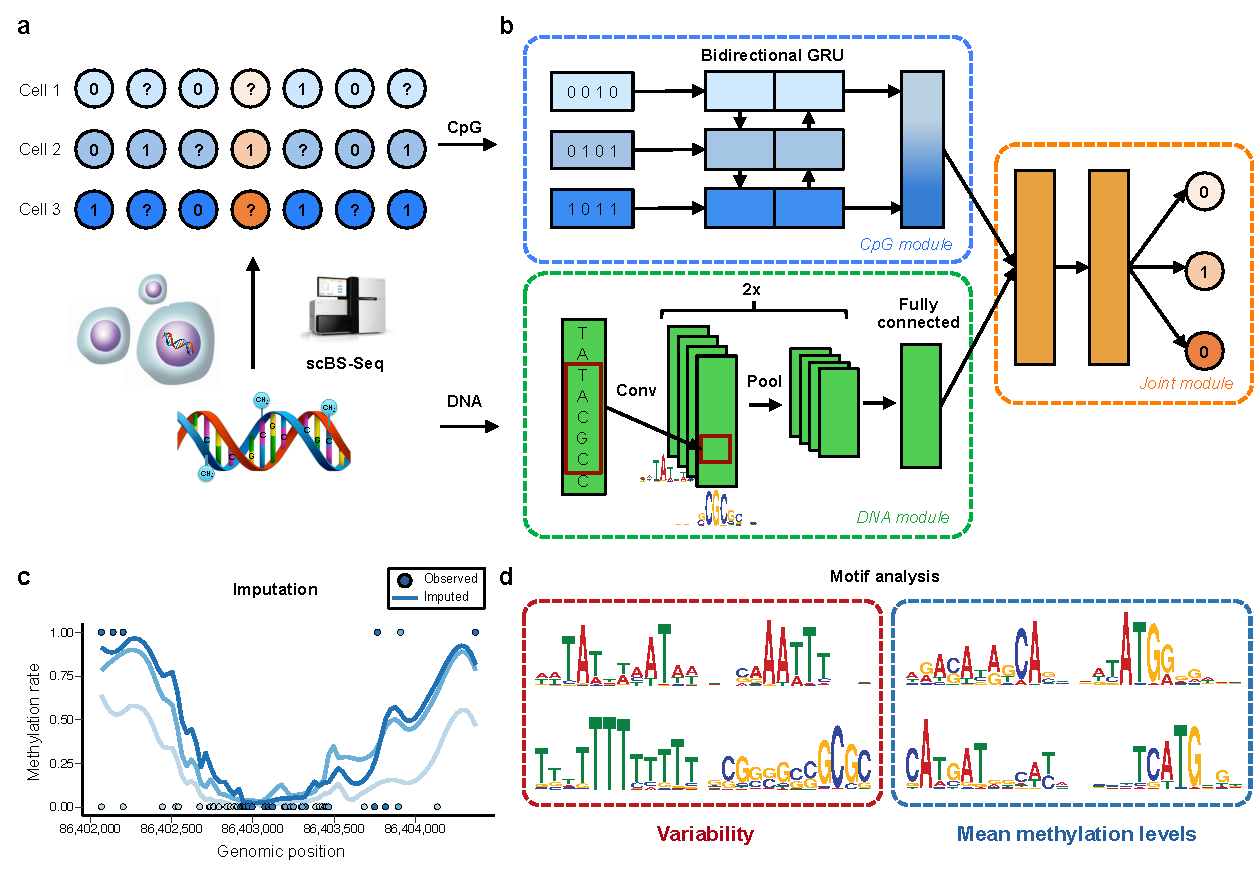
\includegraphics[width=1.0\textwidth]{method}
\caption[DeepCpG model training and applications.]{DeepCpG model training and applications. (a) Sparse single-cell CpG profiles as obtained from scBS-seq (\Cref{sec:bs}) or scRRBS-seq~\citep{farlik_single-cell_2015,guo_profiling_2015,hou_single-cell_2016}. Methylated CpG sites are denoted by ones, un-methylated CpG sites by zeros, and question marks denote CpG sites with unknown methylation state (missing data). (b) Modular architecture of DeepCpG. The DNA module consists of two convolutional and pooling layers to identify predictive motifs from the local sequence context, and one fully connected layer to model motif interactions. The CpG module scans the CpG neighbourhood of multiple cells (rows in b), using a bidirectional GRU (\Cref{sec:dl_rnn}), yielding compressed features in a vector of constant size. The joint module learns interactions between higher-level features derived from the DNA- and CpG module to predict methylation states in all cells. (c, d) The trained DeepCpG model can be used for different downstream analyses, including genome-wide imputation of missing CpG sites (c) and the discovery of DNA sequence motifs that are associated with DNA methylation levels or cell-to-cell variability (d).}
\label{fig:dcpg_method}
\end{figure}

DeepCpG predicts binary CpG methylation states from local DNA sequence windows and observed neighbouring methylation states (\Cref{fig:dcpg_method}~(a)). A major feature of the model is its modular architecture, consisting of a CpG module to account for correlations between CpG sites within and across cells, a DNA module to detect informative sequence patterns, and a joint module that integrates the evidence from the CpG and DNA module to predict methylation states at target CpG sites (\Cref{fig:dcpg_method}~(b)).


\subsection{DNA module}

The DNA module is a CNN (\Cref{sec:dl_cnn}) consisting of a stack of convolutional and pooling layers, which is followed by one fully connected hidden layer. CNNs are designed to extract features from high-dimensional inputs while keeping the number of model parameters tractable by applying a series of convolutional and pooling operations. Unless stated otherwise, the DNA module takes as input a 1001~bp long DNA sequence centred on a target CpG site $n$, which is represented as a binary matrix $s_n$ by one-hot encoding the $D=4$ nucleotides as binary vectors $A=[1, 0, 0, 0]$, $T=[0, 1, 0, 0]$, $G=[0, 0, 1, 0]$, and $C=[0, 0, 0, 1]$. The input matrix $s_n$ is first transformed by a one-dimensional convolutional layer, which computes the activation $a_{nfi}$ of multiple convolutional filters $f$ at every position $i$ within the DNA sequence window:
\begin{align} \label{eq:dcpg_filter_act}
  a_{nfi}=\operatorname{ReLU}(\sum_{l=1}^L \sum_{d=1}^D w_{fld} s_{n,i+l,d})
\end{align}
Here, $w_f$  are the parameters or weights of convolutional filter $f$ of length $L$. These can be interpreted similarly to position weight matrices, which are matched against the input DNA sequence window $s_n$ at every position $i$ to recognize distinct motifs. The $\operatorname{ReLU}(x)=\max(0,x)$ activation function sets negative values to zero, such that $a_{nfi}$ corresponds to the evidence that the motif represented by $w_f$ occurs at position $i$.

A pooling layer is used to summarize the activations of $P$ adjacent neurons by their maximum value:
\begin{align}
  p_{nfi}=\max_{|k|<P/2}(a_{nf,i+k})
\end{align}
Non-overlapping pooling is applied with step size $P$ to decrease the dimension of the input sequence and hence the number of model parameters. The DNA module has multiple pairs of convolutional-pooling layers to learn higher-level interactions between sequence motifs, which are followed by one final fully connected layer with a ReLU activation function. The number of convolutional-pooling layers is a hyperparameter, which was selected by optimizing the prediction performance on the validation set (\Cref{sec:dl_hyper}).


\subsection{CpG module}

The CpG module consists of a non-linear embedding layer to model dependencies between CpG sites within cells, which is followed by a bidirectional GRU (\Cref{sec:dl_rnn}) to model dependencies between cells. Inputs are $100d$ vectors $x_1,\ldots,x_T$, where $x_t$ represents the methylation state and distance of $K=25$ CpG sites to the left and to the right of a target CpG site in cell $t$. Distances were transformed to relative ranges by dividing by the maximum genome-wide distance. The embedding layer is fully connected and transforms $x_t$ into a $256d$ vector $\bar{x}_t$, which allows learning possible interactions between methylation states and distances within cell $t$:
\begin{align}
  \bar{x}_t=\operatorname{ReLU} (W x_t + b)
\end{align}
The sequence of vectors $\bar{x}_t$ are then fed into a bidirectional GRU, which scans input sequence vectors $\bar{x}_1,\ldots,\bar{x}_T$ from left to right, and encodes them into fixed-size hidden state vectors $h_1,\ldots,h_T$:
\begin{align}
  &r_t=\operatorname{sigmoid}(W_{rx} \bar{x}_t + W_{rh} h_{t-1} + b_{r}) \nonumber \\
  &u_t=\operatorname{sigmoid}(W_{ux} \bar{x}_t + W_{uh} h_{t-1} + b_{u}) \nonumber \\
  &\tilde{h}_t=\operatorname{tanh}\left(W_{\tilde{h}x} \bar{x}_t + W_{\tilde{h}h}(r_t \odot h_{t-1}) + b_{\tilde{h}}\right) \nonumber \\
  &h_t = (1 - u_t) \odot h_{t-1} + u_t \odot \tilde{h}_t
\end{align}
The reset gate $r_t$ and update gate $u_t$ determine the relative weight of the previous hidden state $h_{t-1}$ and the current input $\bar{x}_t$ for updating the current hidden state $h_t$. The last hidden state $h_T$ summarizes the sequence as a fixed-size vector. Importantly, the set of parameters $W$ and $b$ are independent of the sequence length $T$, which enables to fine-tune a pre-trained CpG module on a new dataset with a different number of cells.

By using a bidirectional GRU, cell-to-cell dependencies are encoded independently of the order of cells. It consists of a forward and backward GRU with $256d$ hidden state vectors $h_t$, which scan the input sequence from the left and right, respectively. The last hidden state vector of the forward and backward GRU are concatenated into a $512d$, which forms the output of the CpG module.


\subsection{Joint module}

The joint module takes as input the concatenated last hidden vectors of the DNA and CpG module, and models interactions between the extracted DNA sequence and CpG neighbourhood features via two fully connected hidden layers with 512 neurons and ReLU activation function. This enables context-dependent smoothing of neighbouring CpG sites and hence modelling of alternatively shaped methylation profiles, for example in promoter or enhancer regions. The output layer of the joint module contains $T$ sigmoid neurons to predict the methylation rate $\hat{y}_{nt}\in(0;1)$ of CpG site $n$ in cell $t$:
\begin{align} \label{eq:dcpg_y}
  \hat{y}_{nt}=\operatorname{sigmoid}(x)=\frac{1}{1+e^{-x}}
\end{align}


\subsection{Model training}

Model parameters were learned on the training set by minimizing the following loss function:
\newcommand{\Xnll}{\operatorname{NLL}_w(\hat{y},y)}
\begin{align}
  L(w)=\Xnll+\lambda_2 \norm{w}_2
\end{align}
Here, the weight-decay hyperparameter $\lambda_2$ penalises large model weights quantified by the L2 norm, and $\Xnll$ denotes the negative log-likelihood, which measures how well the predicted methylation rates $\hat{y}_{nt}$ fit to observed binary methylation states $y_{nt}\in\{0,1\}$:
\begin{align}
  \Xnll=\sum_{n=1}^N \sum_{t=1}^T o_{nt}\left[y_{nt} \log(\hat{y}_{nt}) + (1-y_{nt}) \log(1-\hat{y}_{nt})\right]
\end{align}
The binary indicator $o_{nt}$ is set to one if the methylation state $y_{nt}$ is observed for CpG site $n$ in cell $t$, and zero otherwise. Dropout (\citep{srivastava_dropout:_2014}; \Cref{sec:dl_overfit}) with different dropout rates for the sequence, CpG, and joint module was used for additional regularization. Model parameters were initialized randomly following the approach in \citet{glorot_understanding_2010}. The loss function was optimized by mini-batch stochastic gradient descent with a batch size of 128 and a global learning rate of 0.0001. The learning rate was adapted by Adam (\citep{kingma_adam:_2014}; \Cref{sec:dl_adapt}), and decayed by a factor of 0.95 after each epoch. Learning was terminated if the validation loss did not improve over ten consecutive epochs (early stopping). The DNA and CpG module were pre-trained independently to predict methylation from the DNA sequence (DeepCpG DNA) or the CpG neighbourhood (DeepCpG CpG). For training the joint module, only the parameters of the hidden layers and the output layers were optimized, whiling keeping the parameters of the pre-trained DNA and CpG module fixed. Training DeepCpG on 18 serum mESCs using a single NVIDIA Tesla K20 GPU took approximately 24 hours for the DNA module, 12 hours for the CpG module, and 4 hours for the joint module. Model hyperparameters were optimized on the validation set by random sampling (\citep{bengio_practical_2012}; \Cref{sec:dl_hyper}).


\subsection{Software availability}

DeepCpG is publicly available on Github\footnote{\url{https://github.com/cangermueller/deepcpg}} and implemented in Python using Theano~\citep{bastien_theano:_2012} and Keras~\citep{chollet_keras:_????}. Our software includes documentation and interactive tutorials on training, evaluating, and analysing DeepCpG. We also provide pre-trained models, which can be efficiently fine-tuned on new data.


\section{Prediction performance evaluation} \label{sec:dcpg_eval}

First, we assessed the ability of DeepCpG to predict single-cell methylation states and compared the model to existing imputation strategies for DNA methylation. As a baseline approach, we considered local averaging of the observed methylation states, either in 3 kb windows centred on the target site of the same cell (WinAvg; \Cref{sec:bs_method}) or across cells at the target site (CpGAvg). Additionally, we compared DeepCpG to a random forest classifier~\citep{breiman_random_2001} trained on individual cells using the DNA sequence information and neighbouring CpG states as input (RF). Finally, we evaluated a recently proposed random forest classifier for predicting methylation rates in bulk populations of cells~\citep{zhang_predicting_2015}, which takes comprehensive DNA annotations into account, including genomic contexts, and tissue-specific regular annotations, such as DNase1 hypersensitivity sites, histone modification marks, and transcription factor binding sites (RF Zhang). All methods were trained, selected, and tested on distinct chromosomes via holdout validation (\Cref{sec:dl_eval}). Specifically, we used chromosomes 1, 3, 5, 7, 9, and 11 as training set, chromosomes 2, 4, 6, 8, 10, and 12 as test set, and the remaining chromosomes as validation set. For each cell type, models were fit on the training set, hyperparameters were optimized on the validation set, and the final model performance and interpretations were exclusively reported on the test set.

Since the proportion of methylated versus unmethylated CpG sites can be unbalanced in globally hypo- or hypermethylated cells, we used the area under the receiver operating characteristics curve (AUC) to quantify the prediction performance of different models. We have also considered a range of alternative metrics, including precision-recall curves, F1 score~\citep{powers_evaluation:_2011}, and Matthews correlation coefficient~\citep{matthews_comparison_1975}, resulting in overall consistent conclusions (\Cref{fig:dcpg_eval_curves}; \Cref{fig:dcpg_eval_dsets_all}).

Initially, we applied all methods to 18 serum-cultured mouse embryonic stem cells (mESCs; average CpG coverage 17.7\%; \Cref{fig:dcpg_eval_cells}), profiled using scBS-seq (\Cref{sec:bs}).

\begin{figure}[htbp!]
\centering
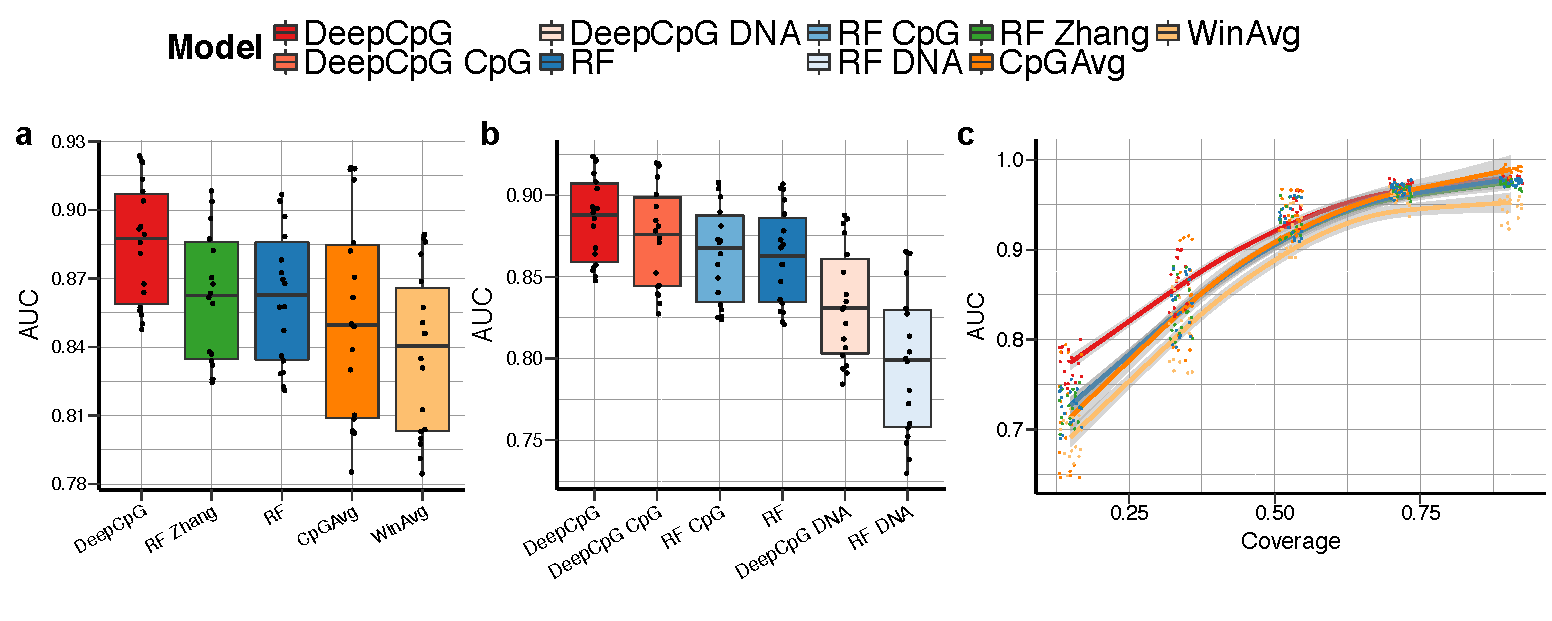
\includegraphics[width=1.0\textwidth]{eval_global}
\caption[Prediction performance of DeepCpG.]{Prediction performance of DeepCpG. (a) Genome-wide prediction performance for 18 serum-grown mouse embryonic stem cells (mESCs) profiled using scBS-seq. Performance is measured by the area under the receiver-operating characteristic curve (AUC), using holdout validation. Considered were DeepCpG, random forest classifiers trained either using DNA sequence and CpG features (RF) or trained using additional annotations from corresponding cell types (RF Zhang). Additionally, two baseline methods were considered, which estimate methylation states by averaging observed methylation states, either across consecutive 3 kb regions within individual cells (WinAvg) or across cells at a single CpG site (CpGAvg). (b) Performance breakdown of DeepCpG and RF, comparing the full models to models trained either only using methylation features (DeepCpG CpG, RF CpG) or DNA features (DeepCpG DNA, RF DNA). (c) AUC of the methods as in (a) stratified by genomic contexts with increasing CpG coverage across cells. Trend lines were fit using local polynomial regression (LOESS); shaded areas denote 95\% confidence intervals.}
\label{fig:dcpg_eval}
\end{figure}

DeepCpG yielded more accurate predictions than any of the alternative methods, both genome-wide and in different genomic contexts (\Cref{fig:dcpg_eval}). Notably, DeepCpG was consistently more accurate than RF Zhang, a model that relies on genomic annotations. These results indicate that DeepCpG can automatically learn higher-level features from the DNA sequence. To investigate this, we tested for associations between the activity of convolutional filters in the DNA module and known sequence annotations (\Cref{sec:dcpg_ana_motifs}), finding both positive and negative correlations with several annotation contexts, including DNase1 hypersensitive sites, histone modification marks, and CpG-rich genomic contexts (\Cref{fig:dcpg_eval_motifs_feat}). The ability to extract higher-level features from the DNA sequence is particularly important for analysing single-cell datasets, where individual cells may be from different cell types and states, making it difficult to derive appropriate annotations.

To assess the relative importance of DNA sequence features compared to neighbouring CpG sites, we trained the same models, however, either exclusively using DNA sequence features (DeepCpG DNA, RF Seq) or neighbouring methylation states (DeepCpG CpG, RF CpG). Consistently with previous studies in bulk populations~\citep{zhang_predicting_2015}, methylation states were more predictive than DNA features, and models trained with both CpG and DNA features performed best (\Cref{fig:dcpg_eval}~(b)). Notably, DeepCpG trained with CpG features alone outperformed a random forest classifier trained with both CpG and DNA features. A likely explanation for the accuracy of the CpG module is its recurrent network architecture, which enables the module to effectively transfer information from neighbouring CpG sites across different cells (\Cref{fig:dcpg_eval_cpg_module}).

\begin{figure}[htbp!]
  \begin{minipage}[c]{0.65\textwidth}
    \centering
    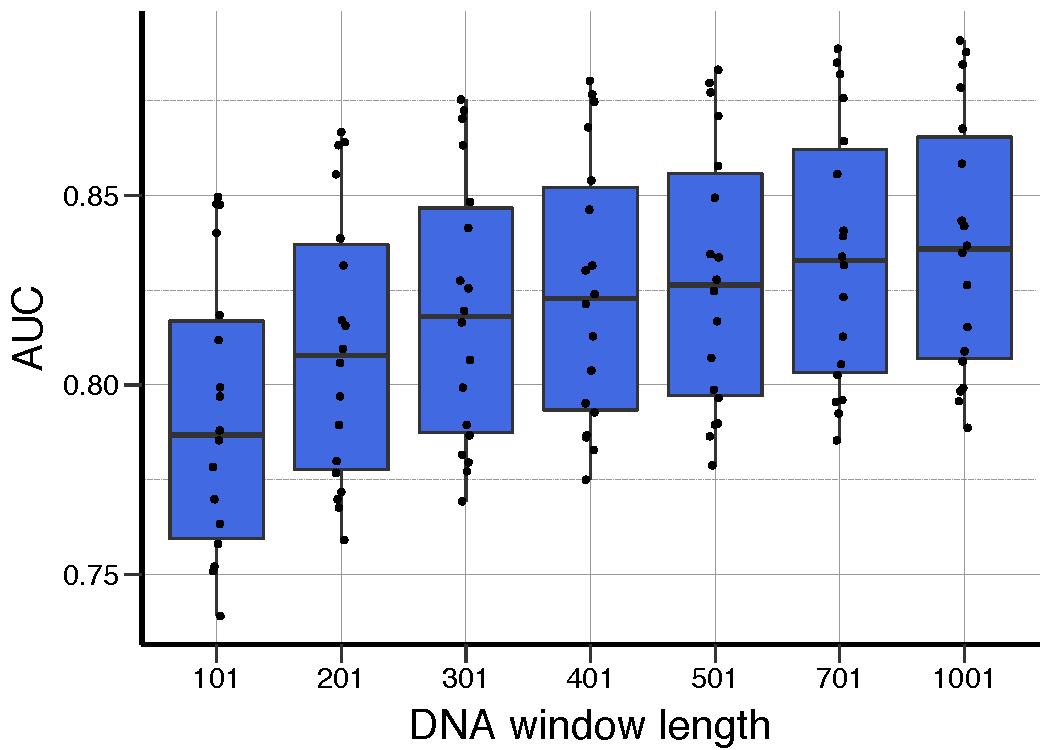
\includegraphics[width=1.0\textwidth]{dna_module_wlen}
  \end{minipage}
  \begin{minipage}[c]{0.32\textwidth}
    \caption[Prediction performance of the DeepCpG DNA module for DNA sequence windows of increasing length.]{Prediction performance of the DeepCpG DNA module for DNA sequence windows of length 101~bp up to 1001~bp.}
    \label{fig:dcpg_eval_dna_module_wlen}
  \end{minipage}
\end{figure}

The largest relative gains between RF and DeepCpG were observed when training both models with DNA sequence information only (AUC 0.83 versus 0.80; \Cref{fig:dcpg_eval}~(b)). This demonstrates the strength of the DeepCpG DNA module to extract predictive sequence features from large DNA sequence windows of up to 1001~bp (\Cref{fig:dcpg_eval_dna_module_wlen}), which is in particular critical for accurate predictions from DNA in uncovered genomic regions, for example when using reduced representation sequencing data~\citep{farlik_single-cell_2015,guo_single-cell_2013,hou_single-cell_2016}. Consistent with this, the relative performance gain of DeepCpG compared to other methods was highest in contexts with low CpG coverage (\Cref{fig:dcpg_eval}~(c); \Cref{fig:dcpg_eval_stats}).

\begin{figure}[htbp!]
\centering
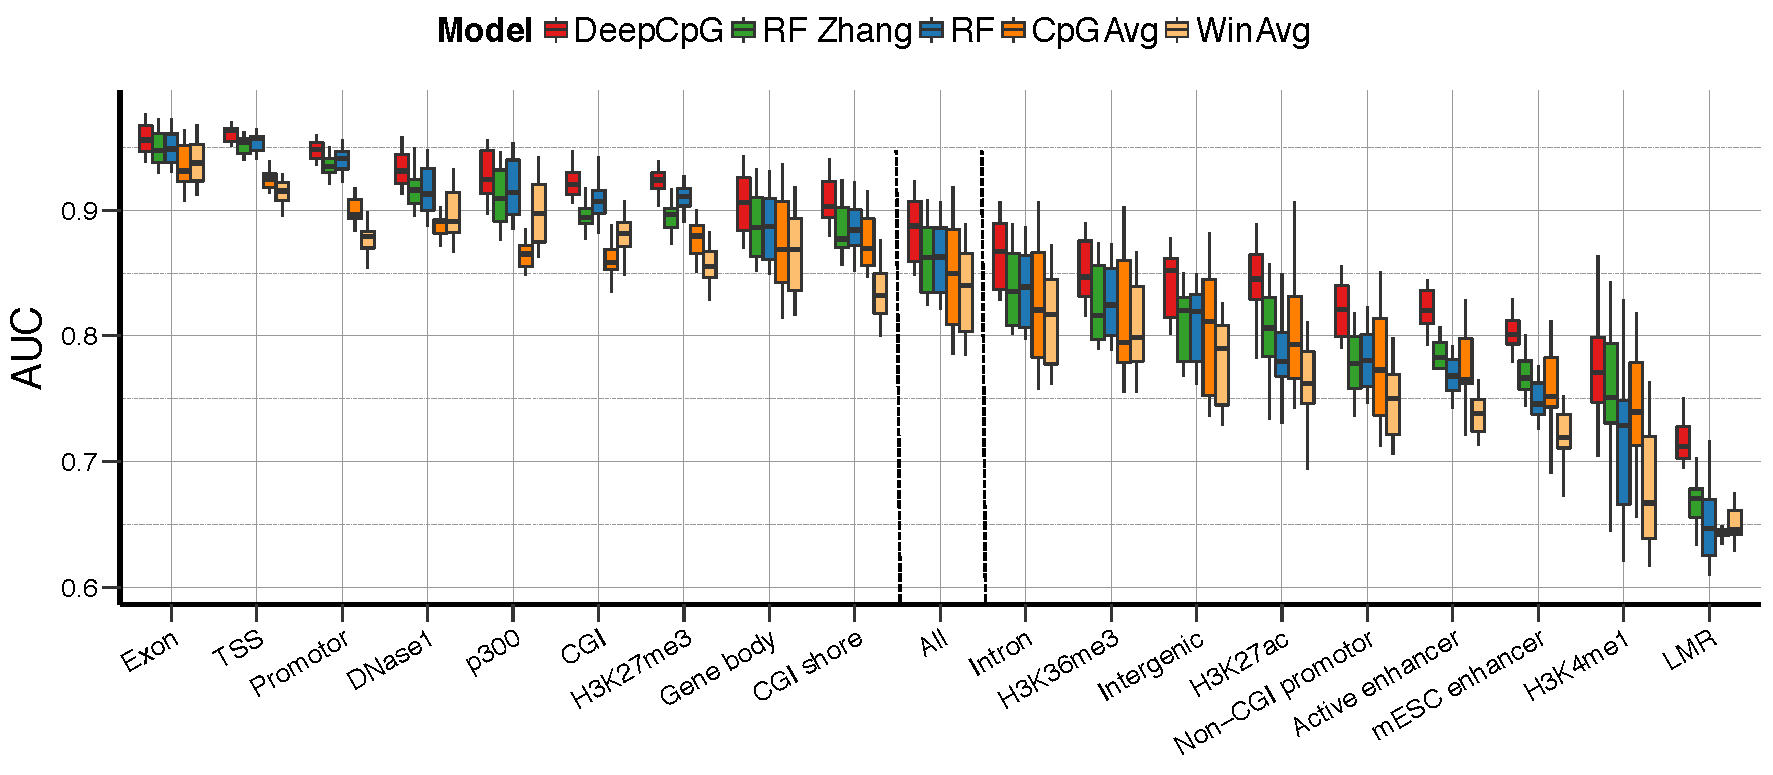
\includegraphics[width=1.0\textwidth]{eval_annos}
\caption[Prediction performance of DeepCpG for alternative genomic contexts.]{Prediction performance of DeepCpG for alternative genomic contexts, with `All' corresponding to genome-wide performances.}
\label{fig:dcpg_eval_annos}
\end{figure}

Next, we explored the prediction performance of all models in different genomic contexts. In line with previous findings~\citep{stevens_estimating_2013,zhang_predicting_2015}, all models performed best in GC-rich contexts (\Cref{fig:dcpg_eval_annos}). However, DeepCpG offered most advantages in GC-poor genomic contexts, including non-CGI promoters, enhancer regions, and histone modification marks (H3K4me1, H3K27ac)--contexts that we found to be associated with higher methylation variability between cells (\Cref{sec:bs_results}).

\begin{figure}[htbp!]
\centering
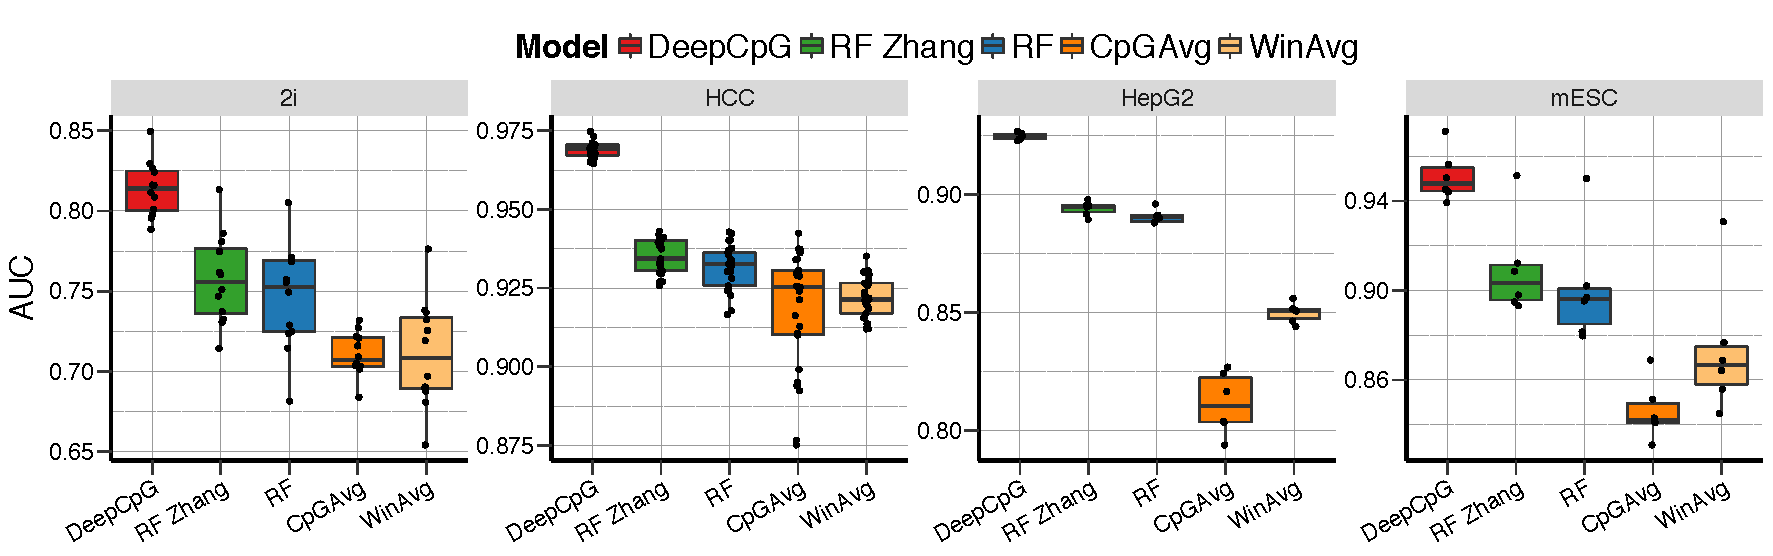
\includegraphics[width=1.0\textwidth]{eval_dsets}
\caption[Prediction performance of DeepCpG for alternative datasets.]{Prediction performance of DeepCpG for alternative datasets. Shown are genome-wide performances for 12 2i-grown mESCs profiled using scBS-seq, as well as three cell types profiled using scRRBS-seq, including 25 human HCC cells, 6 HepG2 cells, and 6 additional mESCs.}
\label{fig:dcpg_eval_dsets}
\end{figure}

We also applied DeepCpG to 12 2i-cultured mESCs profiled using scBS-seq and to data from three cell types profiled using scRRBS-seq~\citep{hou_single-cell_2016}, including 25 human hepatocellular carcinoma cells (HCC), 6 human heptoplastoma-derived (HepG2) cells, and an additional set of 6 mESCs. Notably, in contrast to the serum cells, the human cell types are globally hypomethylated (\Cref{fig:dcpg_eval_cells}). Across all cell types, DeepCpG yielded substantially more accurate predictions than alternative methods (\Cref{fig:dcpg_eval_dsets}; \Cref{fig:dcpg_eval_dsets_all}), demonstrating the broad applicability of the model, including to hypo- and hypermethylated cells, as well to data generated using different sequencing protocols.


\section{Discussion}

We have developed a deep neural network, \emph{DeepCpG}, for predicting DNA methylation in single cells. We have demonstrated that our model enables accurate imputation of missing methylation states, thereby facilitating genome-wide downstream analyses. DeepCpG offers major advantages in shallow sequenced cells as well as in sparsely covered sequence contexts with increased methylation variability between cells. Our method may also help to reduce the required sequencing depth in single-cell bisulfite sequencing studies, thereby enabling the analysis of larger numbers of cells at reduced cost.

The increased accuracy of DeepCpG comes at the expense of higher compute costs. Training DeepCpG genome-wide on a single GPU takes about two days, which is considerably longer compared with conventional machine learning models. However, parallelising computations across multiple GPUs and compute nodes can drastically reduce the training time. Since DeepCpG processes all cells simultaneous, it further shares computations across cells and hence scales better than existing methods to data sets with many cells. Faster training is also possible by only fine-tuning a model that was pre-trained on a related cell type instead of training a new model from scratch.

An important area of future work is to simultaneously impute multiple bulk and single-cell methylation profiles, and to integrate different data modalities from parallel-profiling methods, which are now becoming increasingly available for multiple molecular layers.

%!TEX root = ../thesis.tex
%*******************************************************************************
%****************************** Third Chapter **********************************
%*******************************************************************************
\chapter{Analysis of deep neural networks for predicting DNA methylation} \label{sec:dcpg_ana}

\ifpdf
    \graphicspath{{Chapter5/Figs/Raster/}{Chapter5/Figs/PDF/}{Chapter5/Figs/}}
\else
    \graphicspath{{Chapter5/Figs/Vector/}{Chapter5/Figs/}}
\fi

Deep neural networks are often criticised as hard to interpret `black-box' models. However, model interpretability is critical in multiple fields, including biology and health care. Hence, several approaches have been developed to interpret the parameters of neural networks (\Cref{sec:dl_inter}; \Cref{sec:dl_genomics}) and to obtain insights into learned features. We adapted some of these approaches to analyse DeepCpG (\Cref{sec:dcpg_model}). In particular, we show that DeepCpG can be applied to discover DNA sequence motifs that are associated with methylation states, to identify variance-associated motifs, and to estimate the effect of single nucleotide mutations on DNA methylation. The presented work is based on \citet{angermueller_accurate_2017}.


\section{Discovering DNA sequence motifs} \label{sec:dcpg_ana_motifs}

As described in \cref{sec:dcpg_model}, DeepCpG consists of a DNA, CpG, and joint module. The DNA module has a convolutional architecture with a series of convolutional and max-pooling layers. The filters of the first convolutional layer recognize DNA sequence motifs similarly to conventional position weight matrices and can be visualised as sequence logos (\Cref{sec:dl_genomics}). Existing approaches for visualizing convolutional filters are either \emph{alignment-based} or \emph{optimization-based}. Alignment-based approaches~\citep{alipanahi_predicting_2015,kelley_basset:_2016,quang_danq:_2016} align DNA sequence fragments that maximally activate a certain convolutional filter and visualize the resulting alignment as sequence logo. Optimization-based approaches~\citep{lanchantin_deep_2016,lanchantin_deep_2016-1} optimize the input DNA sequence by gradient descent to maximize the activation of a certain convolutional filter. Our approach is alignment-based. Specifically, we computed the activations $a_{nfi}$ of all filters $f$ of the first convolutional layer for input sequences $s_n$ at every position $i$. We selected sequence window $s_{n,i-L},\ldots,s_{n,i+L}$, if the activation $a_{nfi}$ of filter $f$ with length $L$ at position $i$ (\Cref{eq:dcpg_filter_act}) was greater than 0.5 of the maximum activation of $f$ over all sequences, i.e. $a_{nfi}>0.5 \max_{ni}(a_{nfi})$. We then aligned all selected sequence fragments and visualized filter alignments as sequence logos using WebLogo~\citep{crooks_weblogo:_2004}.

\begin{figure}[htbp!]
\centering
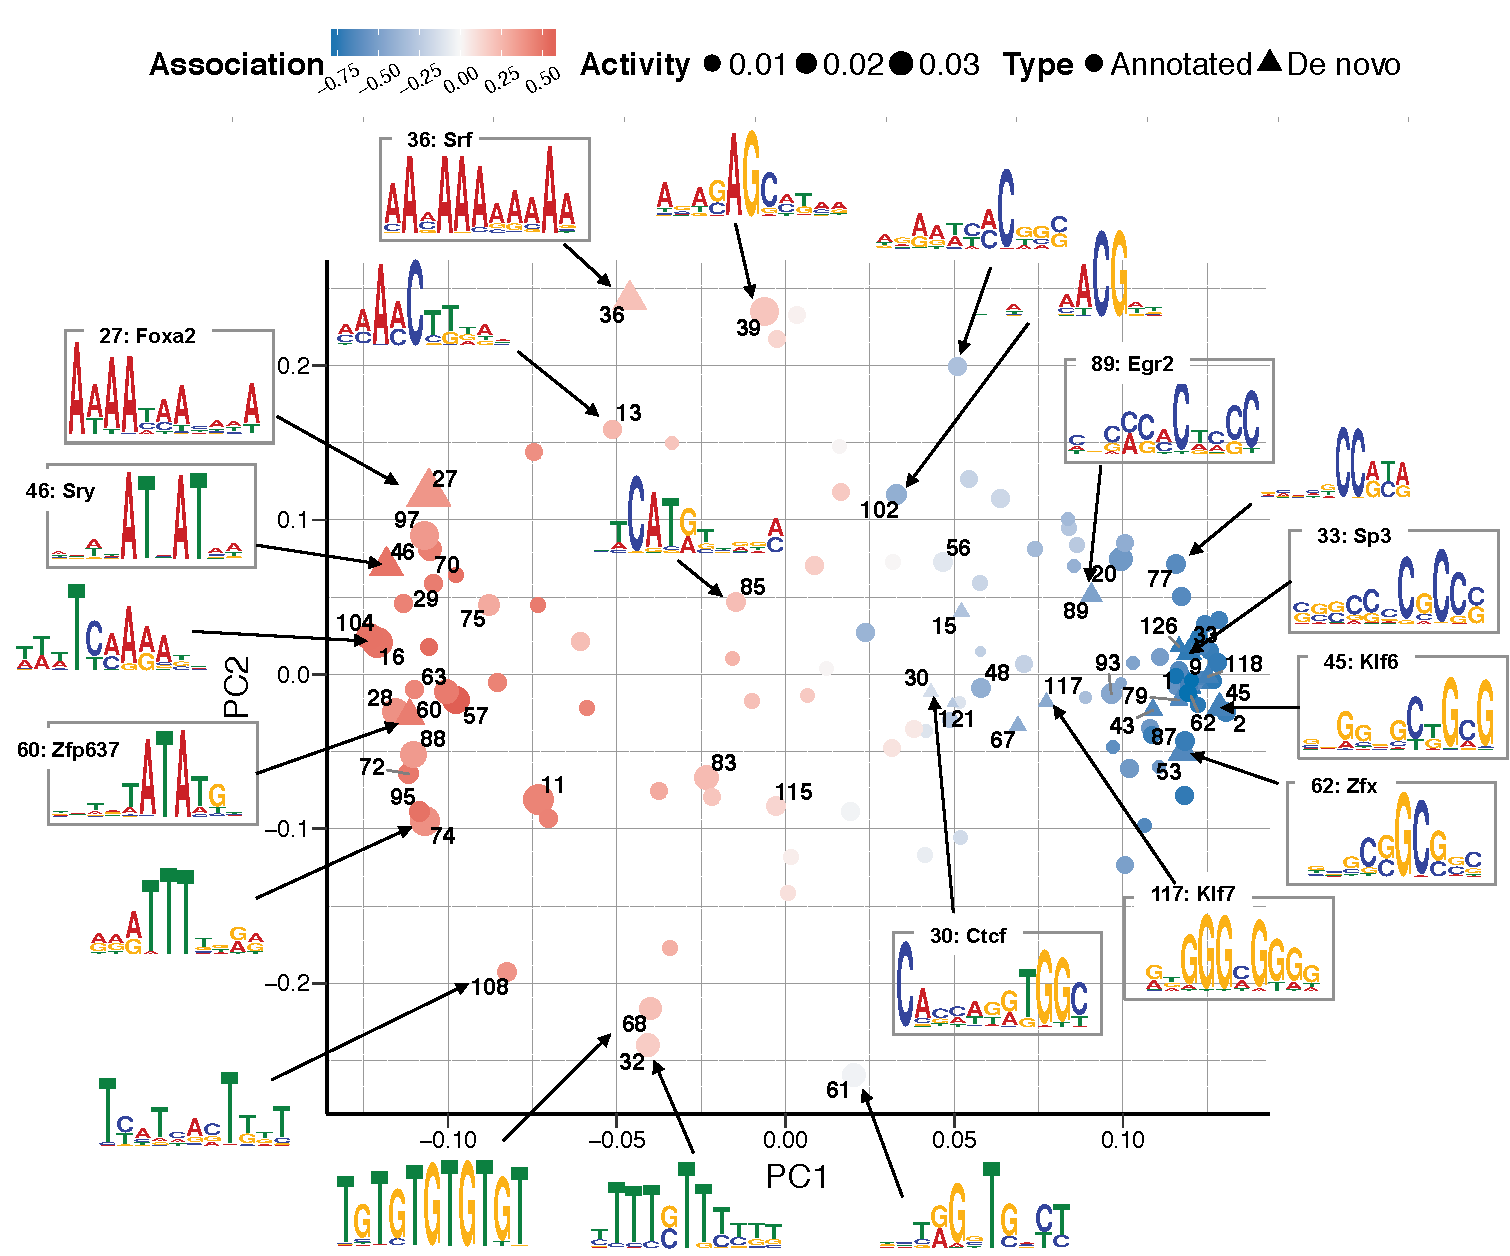
\includegraphics[width=0.9\textwidth]{motifs_pca}
\caption[Principal component analysis of discovered DNA sequence motifs.]{Principal component analysis of discovered DNA sequence motifs. Clustering of 128 motifs discovered by DeepCpG. Shown are the first two principal components of the motif occurrence frequencies in sequence windows (activity). Triangles denote motifs with significant ($\FDR<0.05$) similarity to annotated motif in the CIS-BP or UniPROPE database. Marker size indicates the average activity; the estimated motif effect on methylation level is shown in colour. Sequence logos are shown for representative motifs with larger effects, including 10 annotated motifs.}
\label{fig:dcpg_motifs_pca}
\end{figure}

The number of motifs that the model learns corresponds to the number of convolutional filters, which is a pre-defined hyperparameter. Depending on the choice of this hyperparameter and the nature of the underlying data, learned motifs can be redundant or only weakly associated with DNA methylation. We therefore quantified the importance of learned motifs by two metrics: their activity (occurrence frequency) and their influence on model predictions (association). Specifically, for a set of sequences, e.g. within a certain genomic context, we computed the average of mean sequence activities $\bar{a}_{nf}$, where $\bar{a}_{nf}$ denotes the weighted mean of activities $a_{nfi}$ across all positions $i$ in the sequence window of length $W$:
\begin{align}
  \bar{a}_{nf}=\frac{1}{\sum_{i=1}^W w_i} \sum_{i=1}^W w_i a_{nfi} \qquad w_i=1-\frac{|i-0.5W|}{0.5W}
\end{align}
$w_i$ are linear weights that are highest close the centre position ($i=0.5W$) of the sequence window. We computed the influence of filter $f$ on the predicted methylation states $\hat{y}_{nt}$ of cell $t$ (\Cref{eq:dcpg_y}) as the Pearson correlation $r_{ft}=\operatorname{cor}_n(\bar{a}_{nf},\hat{y}_{nt})$ over CpG sites $n$, and the mean influence $r_f$ over all cells by averaging $r_{ft}$.

\begin{figure}[htbp!]
\centering
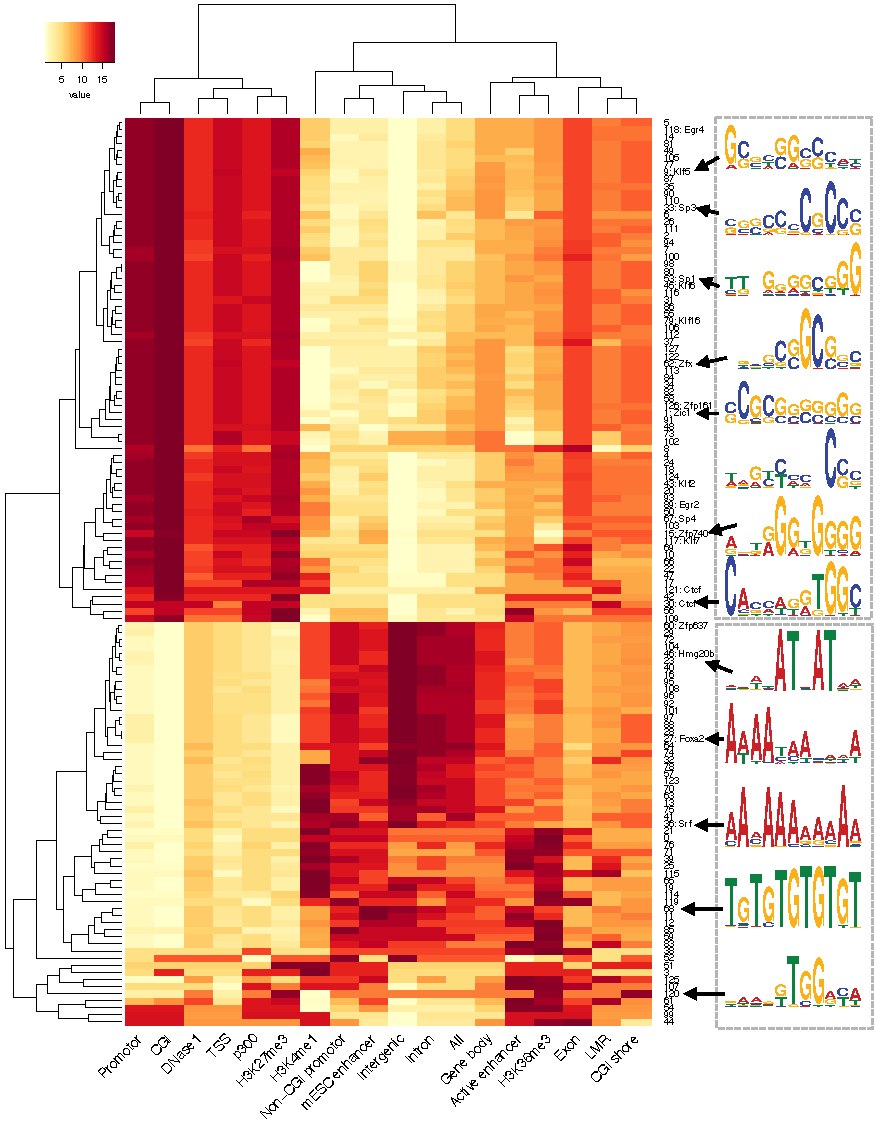
\includegraphics[width=0.8\textwidth]{motifs_act}
\caption[Activity of DNA sequence motifs in genomic contexts.]{Activity of DNA sequence motifs in genomic contexts. Rank of motif activities in different genomic contexts on test chromosomes. The highest activity of CG rich motifs is observed in GC-rich regions such as promotors and CpG islands (CGI). Conversely, the highest activity of AT rich motifs is observed in GC-poor regions such as intergenic or active enhancer regions.}
\label{fig:dcpg_motifs_act}
\end{figure}

To investigate the co-occurrence of motifs across sequence windows, we applied principal component analysis (\Cref{fig:dcpg_motifs_pca}) and hierarchical clustering (\Cref{fig:dcpg_motifs_act}) to motif activities.  Motifs with similar nucleotide composition tended to co-occur in the same sequence windows, where two major motif clusters were associated with increased or decreased methylation levels (\Cref{fig:dcpg_motifs_pca}; \Cref{fig:dcpg_motifs_cor}). Consistent with previous findings~\citep{mendenhall_gc-rich_2010,thomson_cpg_2010,whitaker_predicting_2015}, we observed that motifs associated with decreased methylation tended to be CG rich and were most active in CG rich promoter regions, transcription start sites, as well as in contexts with active promoter marks, such as H3K4me3 or p300 sites (\Cref{fig:dcpg_motifs_act}). Conversely, motifs associated with increased methylation levels tended to be AT rich and were most active in CG poor genomic contexts (\Cref{fig:dcpg_motifs_act}).

We further compared learned motifs, i.e. the weights of the first convolutional layer, to known motifs using Tomtom~\citep{bailey_meme_2009}. 20 out of the 128 learned motifs matched significantly ($\FDR<0.05$) motifs annotated in the Mus Musculus CIS-BP~\citep{weirauch_determination_2014} and UniPROBE~\citep{newburger_uniprobe:_2009} database. 17 of these motifs were transcription factors with a known implication in DNA methylation~\citep{hervouet_dnmt3/transcription_2009,luu_disclosing_2013,whitaker_predicting_2015}, including CTCF~\citep{kim_analysis_2007}, E2f~\citep{tsai_mouse_2008}, and members of the Sp/KLF family~\citep{fernandez-zapico_functional_2011}--transcription factors and regulators of cell differentiation. 13 out of the 20 annotated motifs had been shown to interact with DNMT3a and DNMT3b~\citep{hervouet_dnmt3/transcription_2009}, two major DNA methylation enzymes. Three motifs have no clear associations with DNA methylation. These included Foxa2~\citep{lee_foxa2_2005,wan_compensatory_2005} and Srf~\citep{arsenian_serum_1998,marais_srf_1993}, which are implicated in cell differentiation and embryonic development, as well as Zfp637~\citep{huang_il-6_2016,quenneville_embryonic_2011}, a zinc finger protein that has recently been linked to spermatogenesis in mouse.


\section{Identifying variance-associated motifs}

DNA sequence motifs can either have similar effects in all cells and thereby influence the mean methylation rate across cells, or they can have cell-specific effects and hence account for the variance between cells. Of particular interests for understanding intercellular differences are variance-associated motifs, which we discerned from motifs that are primarily associated with mean methylation levels.

\begin{figure}[htbp!]
\centering
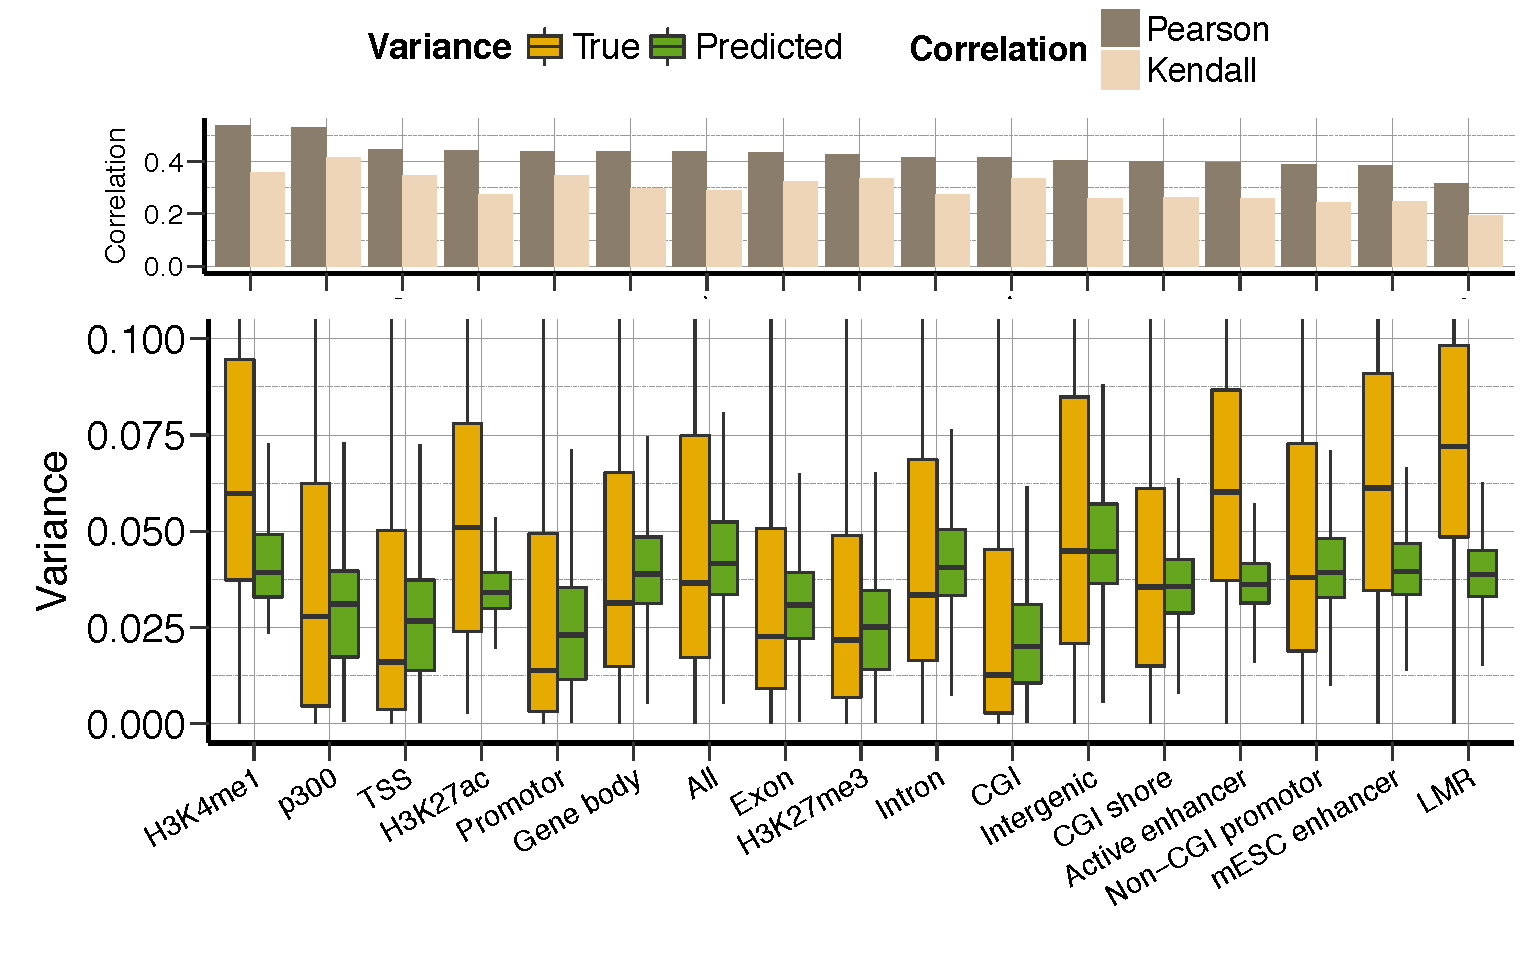
\includegraphics[width=1.0\textwidth]{var_var}
\caption[Performance of DeepCpG DNA module to predict methylation variability.]{Performance of DeepCpG DNA module to predict methylation variability. Boxplot represent predicted (green) and the observed (orange) methylation variability in 3~kbp windows centred on individual CpG sites for different genomic contexts on held out test chromosomes. Barplot represent Pearson and Kendall correlation coefficients.}
\label{fig:dcpg_var_var}
\end{figure}

For this purpose, we trained a second neural network that had the same architecture and in particular reused the motifs from the DNA module of DeepCpG. However, this network was now trained to predict for single CpG sites the variability across cells and the mean methylation rate. Specifically, we replaced output neurons by neurons with a sigmoid activation function to predict for CpG site $n$ both the mean methylation rate $\hat{m}_{ns}$ and cell-to-cell variance $\hat{v}_{ns}$ within a window of size $s\in\{1000,2000,3000,4000,5000\}$~bp. We used multiple window sizes to obtain predictions at different scales, thereby mitigating the uncertainty of mean- and variance estimates in low-coverage regions. For training the resulting model, we initialized and fine-tuned parameters with the corresponding parameters of the DNA module, except for motif parameters of the first convolutional layer. The training objective was
\newcommand{\Xmse}{\operatorname{MSE}}
\begin{align}
  L(w)=\Xmse_w (\hat{m},m,\hat{v},v)+\lambda_2 \norm{w}_2,
\end{align}
where $\Xmse$ the is mean squared error between model predictions and training labels:
\begin{align}
  \Xmse_w(\hat{m},m,\hat{v},v)=\sum_{n=1}^{N}\sum_{s=1}^S (m_{ns}-\hat{m}_{ns})^2+(v_{ns}-\hat{v}_{ns})^2
\end{align}
$m_{ns}$ is the estimated mean methylation rate for a window centred on target site n of a certain size indexed by $s$:
\begin{align}
  m_{ns}=\frac{1}{T}\sum_{t=1}^T m_{nst}
\end{align}
Here, $m_{nst}$ denotes the estimated mean methylation rate of cell $t$ computed by averaging the binary methylation state $y_{it}$ in the set of all observed CpG sites $Y_{nst}$ in window $s$
\begin{align}
  m_{nst}=\frac{1}{|Y_{nst}|} \sum_{i \in Y_{nst}} y_{it},
\end{align}
where $v_{ns}$ denotes the estimated cell-to-cell variance:
\begin{align}
  v_{ns}=\frac{1}{T} \sum_{t=1}^T (m_{nst}-m_{ns})^2
\end{align}
We evaluated this model by holdout validation as we did before (\Cref{sec:dcpg_eval}). Notably, the model could predict both global changes in mean methylation levels (Pearson's $R=0.80$; $\operatorname{MAD}=0.01$; \Cref{fig:dcpg_var_mean}), as well as cell-to-cell variability (Pearson's $R=0.44$; $\operatorname{MAD}=0.03$, \cref{fig:dcpg_var_var}; Kendall's $R=0.29$, \cref{fig:dcpg_var_rank}).

\begin{figure}[htbp!]
\centering
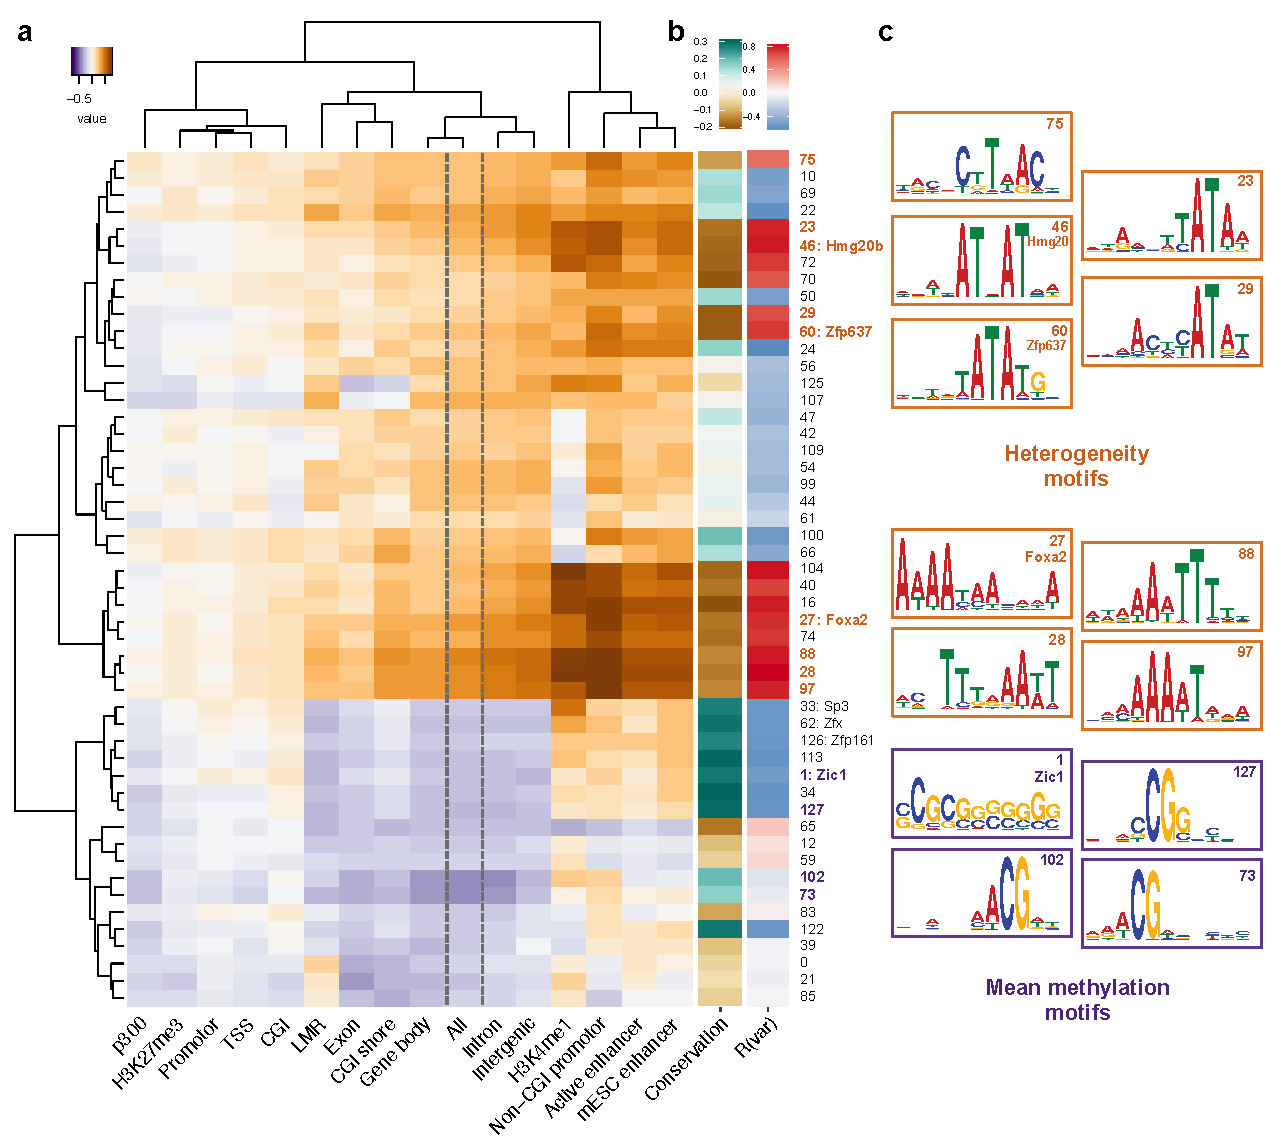
\includegraphics[width=1.0\textwidth]{var_motifs}
\caption[Identification of motifs associated with mean methylation levels and cell-to-cell variability.]{Identification of motifs associated with mean methylation levels and cell-to-cell variability. (a) Difference of motif effect on cell-to-cell variability and methylation levels for different genomic contexts. Motifs associated with increased cell-to-cell variability are highlighted in brown; motifs that were primarily associated with changes in methylation level are shown in purple. (b) Genome-wide correlation coefficients between motif activity and DNA sequence conservation (left), as well as cell-to-cell variability (right). (c) Sequence logos for selected motifs identified in (a), which are highlighted by colour in (b).}
\label{fig:dcpg_var_motifs}
\end{figure}

There is an intrinsic mean-variance relationship of single-cell methylation states (\Cref{fig:dcpg_var_couple}), and hence the separation of the motif impact on mean methylation and methylation variance is partially confounded. To mitigate this effect, we used a scoring approach that separates the effect of individual motifs on cell-to-cell variability and mean methylation levels. Specifically, we computed the influence $r^v_{fs}$ of filter $f$ on cell-to-cell variability in widows of size $s$ as the Pearson correlation between mean sequence filter activities $\bar{a}_{nf}$ and predicted variance levels $\hat{v}_{ns}$ of sites $n$:
\begin{align}
  r^v_{fs}=\operatorname{cor}_n(\bar{a}_{nf},\hat{v}_{ns})
\end{align}
Analogously, we computed the influence $r^m_{fs}$ on predicted mean methylation levels $\hat{m}_{ns}$. We then used the difference $r^d_{fs}=|r^v_{fs}|-|r^m_{fs}|$ between the absolute value of the influence on variance and mean methylation levels to identify motifs that were primarily associated with cell-to-cell variance $r^d_{fs}>0.25$, or with changes in mean methylation levels $r^d_{fs}<-0.25$.

\begin{figure}[htbp!]
\centering
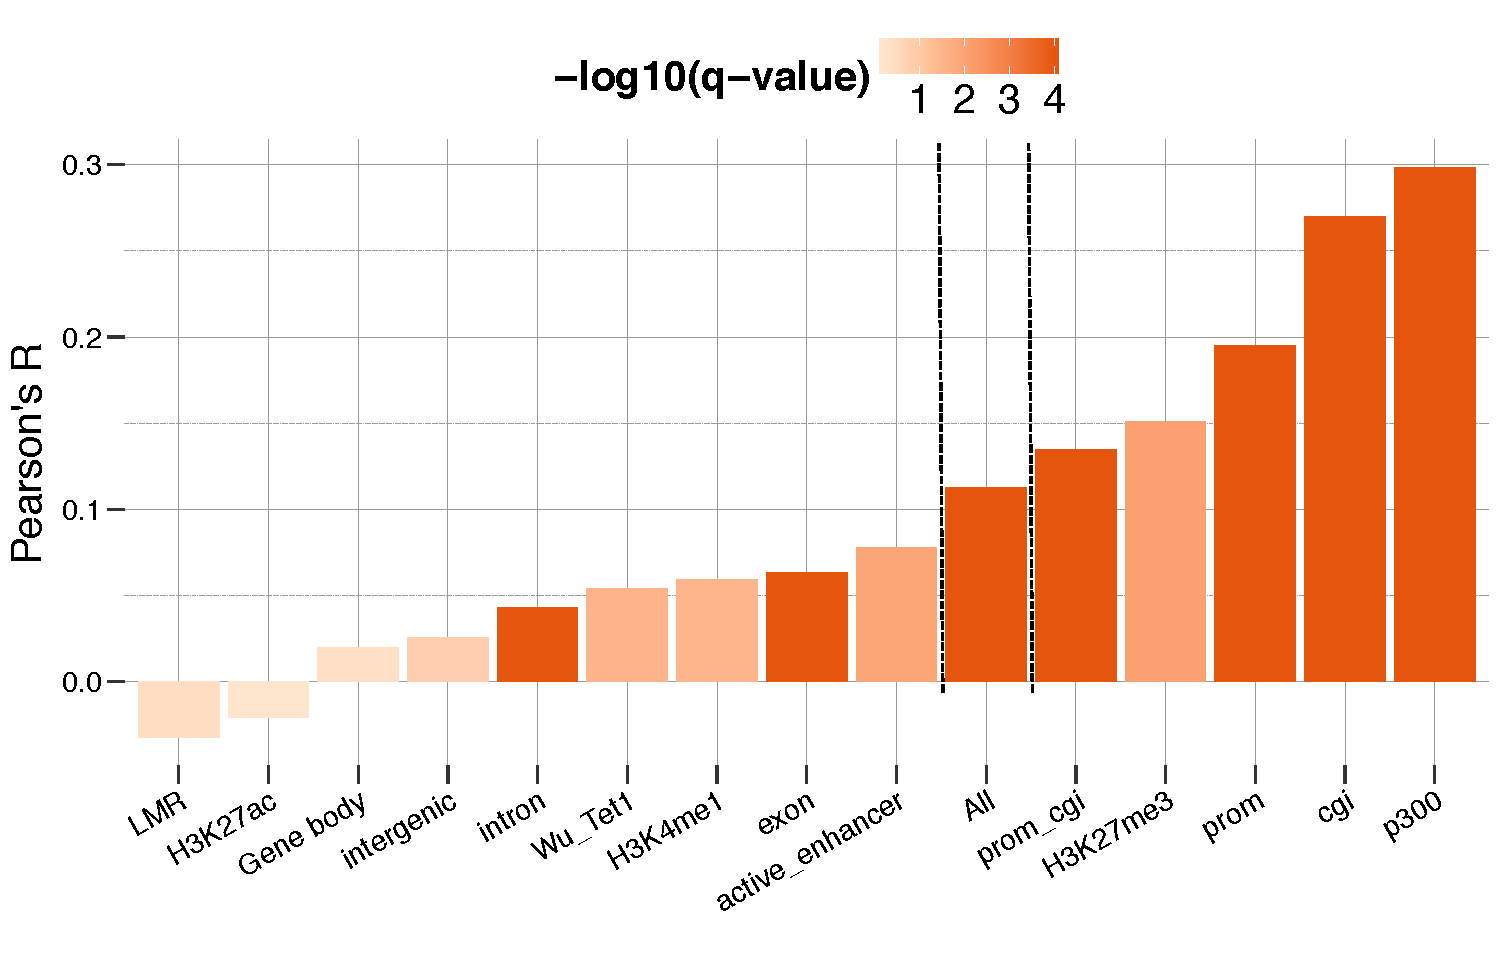
\includegraphics[width=0.8\textwidth]{var_mt}
\caption[Functional assessment of predicted cell-to-cell variability.]{Functional assessment of predicted cell-to-cell variability. Pearson correlation coefficient between methylome-transcriptome linkage as reported in \cref{sec:mt}, and the predicted cell-to-cell variability for test chromosomes. Colour denotes statistical significance (q-value, Benjamini Hochberg adjusted). Significant correlations ($\FDR<0.01$) were observed  genome-wide (`All') and in most genomic contexts.}
\label{fig:dcpg_var_mt}
\end{figure}

The approach identified 22 motifs that were primarily associated with cell-to-cell variance (\Cref{fig:dcpg_var_motifs}). These motifs tended to be active in CG-poor and active enhancer regions--sequence contexts with increased epigenetic variability (\Cref{sec:bs_results}). 12 of the identified motifs were AT-rich and associated with increased variability, including the differentiation factors Foxa2~\citep{lee_foxa2_2005,wan_compensatory_2005}, Hmg20b~\citep{sumoy_hmg20a_2000}, and Zfp637~\citep{huang_il-6_2016,quenneville_embryonic_2011}. Notably, variance-increasing motifs were more frequent in un-conserved regions such as active enhancers, in contrast to variance-decreasing motifs, which were enriched in evolutionary conserved regions such as gene promoters (\Cref{fig:dcpg_var_motifs}~(b); \Cref{fig:dcpg_var_cons}). Our analysis also revealed 4 motifs that were primarily associated with mean methylation levels, which were in contrast CG rich and most active in conserved regions.

To explore whether the model predictions for variable sites are functionally relevant, we overlaid predictions with methylome-transcriptome linkages from our previous study (\Cref{sec:mt}). The rationale behind this approach is that regions with increased methylation variability are more likely to harbour associations with gene expression. Consistent with this hypothesis, we observed a weak but globally significant association (Pearson's $R=0.11$; $P=5.72\times10^-16$; \Cref{fig:dcpg_var_mt}).

\section{Estimating the effect of DNA mutations}

\begin{figure}[htbp!]
\centering
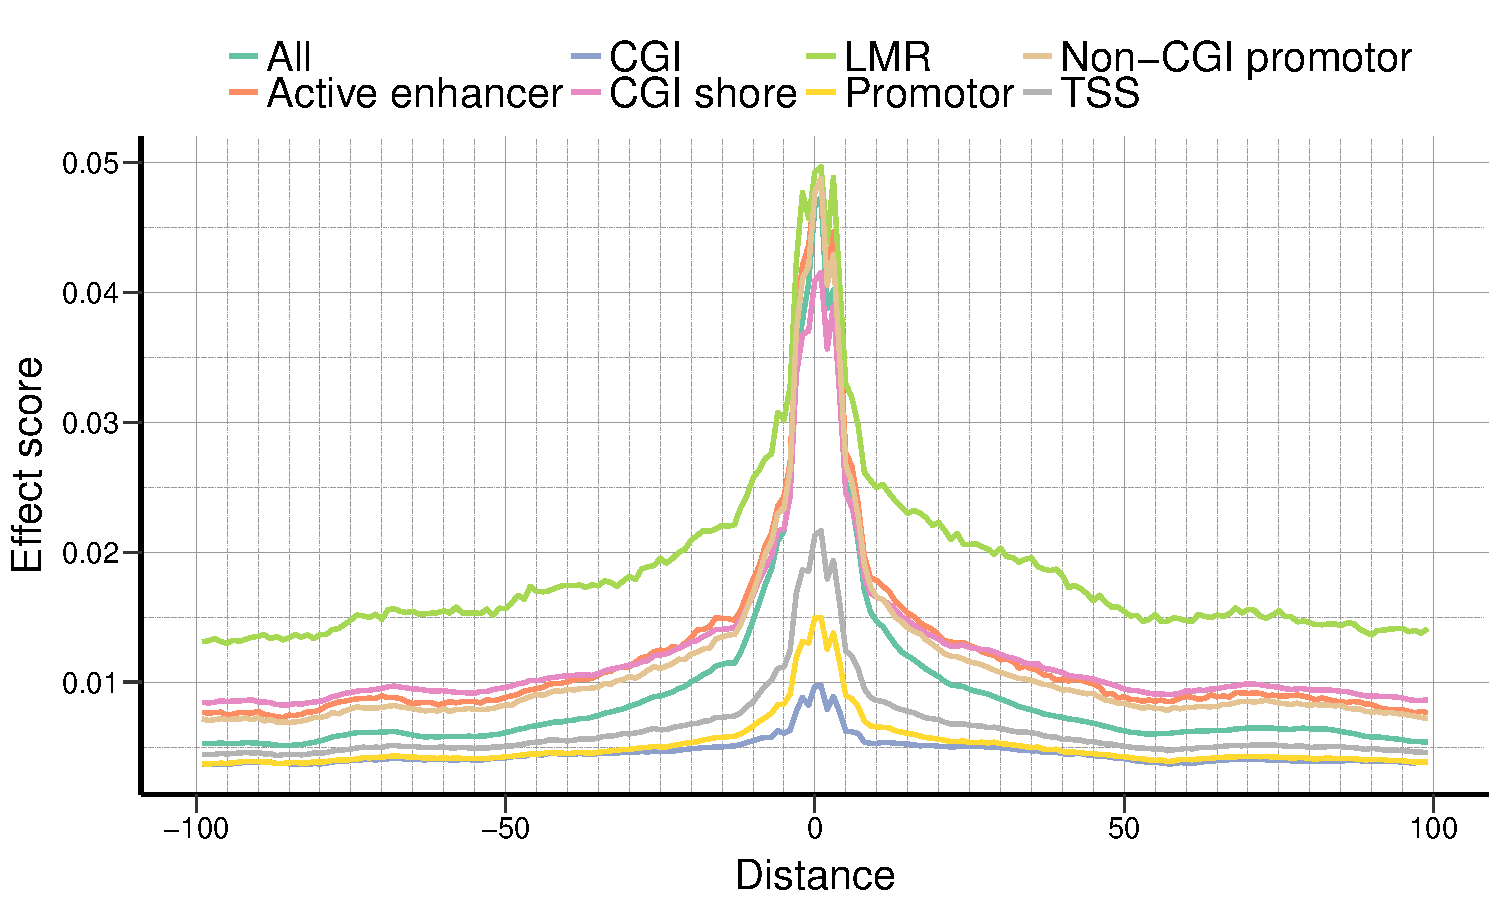
\includegraphics[width=0.9\textwidth]{mut_global}
\caption[Average genome-wide effect of single nucleotide mutations on CpG methylation estimated using DeepCpG.]{Average genome-wide effect of single nucleotide mutations on CpG methylation estimated using DeepCpG, depending on the distance to the CpG site and the genomic context.}
\label{fig:dcpg_mut_global}
\end{figure}

The trained DeepCpG model can also be used to estimate the effect of single nucleotide mutations on CpG methylation. For this purpose, we adapted a gradient-based approach~\citep{simonyan_deep_2013} to estimate mutational effects in a computationally efficient manner, thereby greatly reducing the compute cost compared to previous methods~\citep{alipanahi_predicting_2015,zhou_predicting_2015,zhou_predicting_2015}. Specifically, let $\hat{y}_n(s_n)=\frac{1}{T}\sum_t \hat{y}_{nt}(s_n)$ be the mean predicted methylation rate across cells $t$ for an input sequence $s_n$. Then we quantified the effect $e^s_{nid}$ of changing nucleotide $d$ at position $i$ as:
\begin{align}
  e^s_{nid}=\frac{\Delta \hat{y}_{nt}(s_n)}{\Delta s_{nid}}(1-s_{nid})
\end{align}
Here, the first term is the first-order gradient of $\hat{y}_n$ with respect to $s_{nid}$, and the second term sets the effect of wild-type nucleotides ($s_{nid}=1$) to zero. We quantified the overall effect score $e^s_{ni}$ at position $i$ as the maximum absolute effect over all nucleotide changes, i.e. $e^s_{ni}=\max_d(|e^s_{nid}|)$.

\begin{figure}[htbp!]
\centering
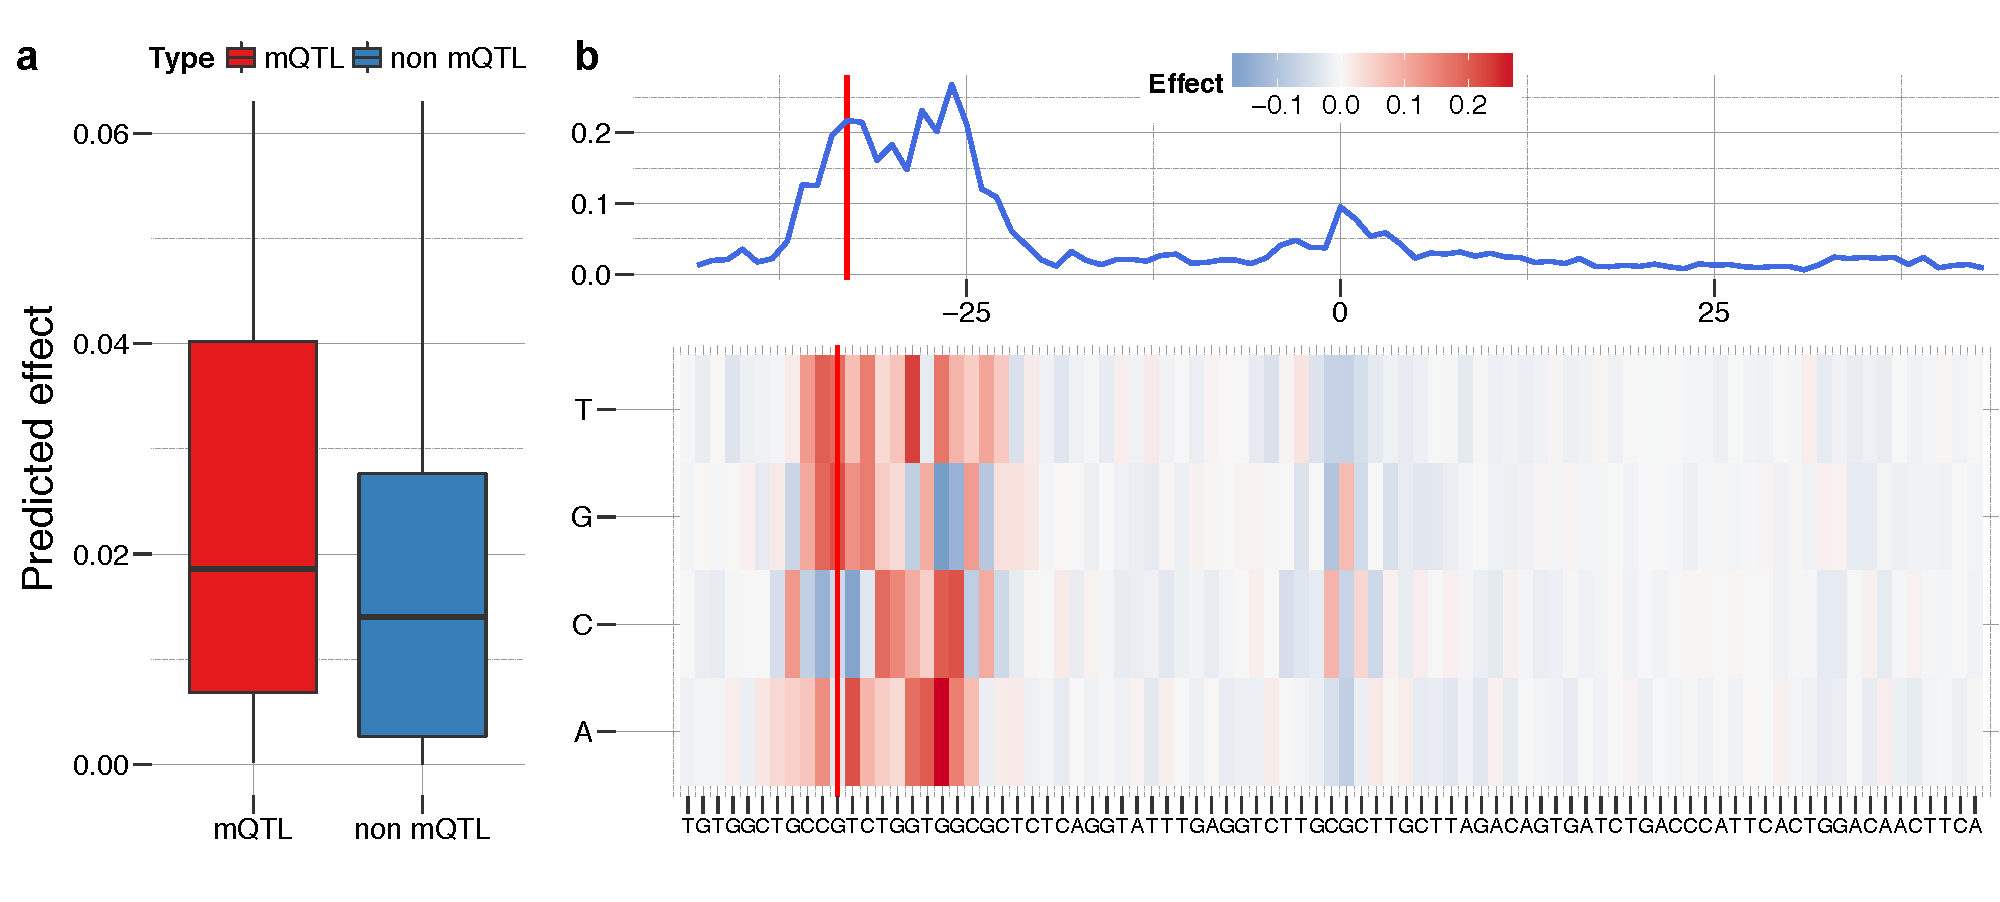
\includegraphics[width=1.0\textwidth]{mut_qtl_zoom}
\caption[Analysis and example visualization of estimated single nucleotide mutation effects for methylation QTLs (mQTLs).]{Analysis and example visualization of estimated single nucleotide mutation effects for methylation QTLs (mQTLs). (a) Distribution of the mutation effect for 2379 mQTLs variants from \citet{kaplow_pooling-based_2015}, compared to distance-matched random variants (non mQTL). (b) Visualization of mutation effects for an example CpG site and the corresponding mQTL. Shown are effects in a window centred on the example CpG site (chromosome 1; position 159791497). The position of the corresponding mQTL from \citet{kaplow_pooling-based_2015} (rs60205880; position 159791464) is indicated by the vertical red line. The heat map in the lower panels shows effect sizes for individual nucleotides, and line plot in the upper panel the maximum absolute effect across nucleotides.}
\label{fig:dcpg_mut_qtl_zoom}
\end{figure}

As expected, mutations in the direct vicinity of the target CpG site had the largest effects (\Cref{fig:dcpg_mut_global}). Mutations in CG dense regions such as CGIs or promoters tended to have smaller effects, suggesting that DNA methylation in these genomic contexts is more robust to single nucleotide mutations. Globally, we observed a negative correlation between mutational effects and DNA sequence conservation ($P<1.0\times10^{-15}$; \Cref{fig:dcpg_mut_cons}), providing evidence that estimated single nucleotide effects capture genuine effects.

We further evaluated mutational effects by comparing the effect for 2379 methylation QTLs (mQTLs) from \citet{kaplow_pooling-based_2015} with the effect for matched non-mQTL variants. Since \citet{kaplow_pooling-based_2015} mapped mQTLs in human cells, we used the DeepCpG model trained on HepG2 cells for this experiments. To adjust of differences in effect due to the distance to the CpG site (\Cref{fig:dcpg_mut_global}), we randomly sampled non-QTLs at distances matched to mQTLs. Known mQTL variants had significantly larger effects than matched random variants ($P<1.0\times10^{-15}$, Wilcoxon rank sum test; \Cref{fig:dcpg_mut_qtl_zoom}), providing evidence that DeepCpG can be used to identify functional variants from the DNA sequence alone.


\section{Discussion}

We have developed alternative approaches for interpreting the parameters of DeepCpG and for obtaining insights into the learned features. We have used these approaches to discover motifs that are associated with DNA methylation states, to identify variance-associated motifs, and to estimate the effect of single nucleotide mutations on DNA methylation.

Although our approaches helped to better understand DeepCpG, they are not free of limitations. First, the randomness that is involved in the training of DeepCpG affects which specific motifs are learned. This applies in particular to the random initialization of the parameters of the first convolutional layer. One way to address this problem is to initialize a fraction of convolutional filters by known DNA sequence motifs, which, however, can introduce biases and decrease prediction accuracy.

Although our approaches helped to better understand DeepCpG, they are not free of limitations. First, the randomness that is involved in the training of DeepCpG affects which specific motifs are learned. This applies in particular to the random initialization of the parameters of the first convolutional layer. One way to address this problem is to initialize a fraction of convolutional filters by known DNA sequence motifs, which, however, requires prior knowledge about methylation-associated motifs for the cell type of interest and can introduce biases.

Second, the model can learn redundant and overlapping motifs depending on the choice of the number of convolutional filters and the dropout rate. More distinct motifs can be obtained by penalizing the number motifs with non-zero weights, analogously to the Bayesian automatic relevance determination framework~\citep{mackay_bayesian_1992,neal_bayesian_2012}.

Third, our scoring approach to identify variance-associated motifs does not fully disentangle the mean-variance relationship of binomial-distributed methylation states in single cells. One approach to more clearly separate between mean and variance motifs would be to model methylation states using a beta-binomial distribution, where mean and over-dispersion parameters are predicted by a deep neural network, similar to mixture density networks~\citep{bishop1994mixture}.

Forth, our gradient-based approach to quantify the effect of single nucleotide mutations is problematic because the ReLU activation function can have a gradient of zero but still transfer information. This problem has recently been addressed by comparing neuron activations to reference activations~\citep{shrikumar_not_2016}--a promising strategy also in the context of DNA methylation. Another avenue of future research is to quantify statistical significance of estimated effect scores, which is important for prioritizing genomic variants.



% ********************************** Back Matter *******************************
% Backmatter should be commented out, if you are using appendices after References
%\backmatter

% ********************************** Bibliography ******************************
\begin{spacing}{0.9}

% To use the conventional natbib style referencing
% Bibliography style previews: http://nodonn.tipido.net/bibstyle.php
% Reference styles: http://sites.stat.psu.edu/~surajit/present/bib.htm

% \bibliographystyle{apalike}
%\bibliographystyle{unsrt} % Use for unsorted references
\bibliographystyle{plainnat} % use this to have URLs listed in References
\cleardoublepage
\bibliography{References/references} % Path to your References.bib file


% If you would like to use BibLaTeX for your references, pass `custombib' as
% an option in the document class. The location of 'reference.bib' should be
% specified in the preamble.tex file in the custombib section.
% Comment out the lines related to natbib above and uncomment the following line.

%\printbibliography[heading=bibintoc, title={References}]


\end{spacing}

% ********************************** Appendices ********************************

\begin{appendices} % Using appendices environment for more functunality

\include{Appendix1/appendix1}
\include{Appendix2/appendix2}

\end{appendices}

% *************************************** Index ********************************
\printthesisindex % If index is present

\end{document}
